\documentclass[nemilov1]{Nemilov}
\usepackage{fix-cm}
\usepackage[english]{babel}
\usepackage{amssymb}
\usepackage{amsmath}
\usepackage{graphicx}
\usepackage{subfigure}
\usepackage{makeidx}
\usepackage{multicol}
\usepackage{inputenc}
\usepackage{epigrafica}
\usepackage[LGR,OT1]{fontenc}
\usepackage{mathptmx}
\usepackage{changepage}
\usepackage[center]{caption}
\usepackage{float}

\hfuzz=30pt % Don't bother to report over-full boxes < 10pt
\vfuzz=30pt % Don't bother to report over-full boxes < 10pt


% Use numbers for nested lists all the way down.
\usepackage{enumitem}
\setlist[enumerate,1]{label=\arabic*., ref=\arabic*}
\setlist[enumerate,2]{label=\arabic*., ref=\arabic*}
\setlist[enumerate,3]{label=\arabic*., ref=\arabic*}

% Allow multi-page tables.
\usepackage{longtable}

% Make description items cross-referenceable
\def\namedlabel#1#2{\begingroup
    #2%
    \def\@currentlabel{#2}%
    \phantomsection\label{#1}\endgroup
}
\makeatother

% Change hanging indentation for description environment.
\makeatletter
\renewenvironment{description}%
  {\list{}{\leftmargin=1em\itemsep3pt % <------- Adjust this length
    \labelwidth\z@ \itemindent-\leftmargin
    \let\makelabel\descriptionlabel}}%
  {\endlist}
\makeatother

% Use smaller font for verbatim environments.
\usepackage{fancyvrb}

% Syntax highlighting with minted <http://mirror.its.dal.ca/ctan/macros/latex/contrib/minted/minted.pdf>
\usepackage{minted}%

\frenchspacing
\tolerance=5000

%----------------------------------------

% Ignore subtitle in PDF version.
\newcommand{\subtitle}[1]{}

% Asides
\newenvironment{aside}[1]%
{\addvspace{6pt}\begin{adjustwidth}{2em}{2em}%
\centerline{\itshape\textbf{#1}}\par\itshape\noindent\ignorespaces}%
{\end{adjustwidth}\addvspace{6pt}}

% Glossary references and items
\newcommand{\gref}[2]{\hyperlink{#1}{\textbf{#2}}}
\newcommand{\gitem}[2]{\item[\hypertarget{#1}{#2}]}

% Remove indentation from footnotes
\usepackage[hang,flushmargin]{footmisc}

%----------------------------------------

% Render hyperlinks with footnotes as well.
\newcommand{\hreffoot}[2]{{#2}\footnote{\href{#1}{#1}}}

% Mark recommendations.
\newcommand{\recommendation}[1]{\emph{#1}}

\usepackage[T1]{fontenc}

% Bibliography.
\usepackage[backend=biber,style=alphabetic,sorting=nyt,maxbibnames=99]{biblatex}
\addbibresource{book.bib}

% https://tex.stackexchange.com/questions/8428/use-bibtex-key-as-the-cite-key
\DeclareFieldFormat{labelalpha}{\thefield{entrykey}}
\DeclareFieldFormat{extraalpha}{}

\setlength{\biblabelsep}{\labelsep}% <-- adjust this to your liking, the standard is 2\labelsep
\defbibenvironment{bibliography}
  {\addcontentsline{toc}{chapter}{\bfseries References}\list
     {\printtext[labelalphawidth]{%
        \printfield{prefixnumber}%
        \printfield{labelalpha}%
        \printfield{extraalpha}}}
     {\setlength{\labelsep}{\biblabelsep}%
      \setlength{\leftmargin}{24pt}%\labelsep
      \setlength{\itemsep}{\bibitemsep}%
      \setlength{\parsep}{\bibparsep}}%
      \renewcommand*{\makelabel}[1]{\bf##1\hss}}
  {\endlist}
  {\item}
\bibparsep3pt

\usepackage{csquotes}
%----------------------------------------

\def\UrlFont{\rmfamily}

% Chapters, sections, and appendices with labels.
\newcommand{\chaplbl}[2]{\chapter{#1}\label{#2}}
\newcommand{\seclbl}[2]{\section{#1}\label{#2}}
\newcommand{\appref}[1]{Appendix~\ref{#1}}
\newcommand{\chapref}[1]{Chapter~\ref{#1}}
\newcommand{\figref}[1]{Figure~\ref{#1}}
\newcommand{\secref}[1]{Section~\ref{#1}}

% Image figures.
\newcommand{\figimg}[3]{\begin{figure}%
\centering%
\includegraphics[width=\textwidth]{#1}%
\caption{#2}%
\label{#3}%
\end{figure}}

% PDF figures.
\newcommand{\figpdf}[3]{\begin{figure}%
\centering%
\includegraphics[scale=0.6]{#1}%
\caption{#2}%
\label{#3}%
\end{figure}}

% PDF figures forcing location.
\newcommand{\figpdfhere}[3]{\begin{figure}[H]%
\centering%
\includegraphics[scale=0.6]{#1}%
\caption{#2}%
\label{#3}%
\end{figure}}

% Exercise headings.
\newcommand{\exercise}[3]{\subsection*{#1 (#2/#3)}}

\setlength{\paperheight}{11in}

%----------------------------------------
 
% Always load hyperref last
% https://tex.stackexchange.com/questions/16268/warning-with-footnotes-namehfootnote-xx-has-been-referenced-but-does-not-exi
\usepackage{hyperref}


\begin{document}

\title{Teaching Tech Together}
\subtitle{How to create and deliver lessons that work\\ and build a teaching community around them}
\author{Greg Wilson}
\date{Version 4.0 beta / June 2019}
\maketitle

\frontmatter
\dedication{
For my mother, Doris Wilson,\\
who taught hundreds of children to read and to believe in themselves.\\
~\\
And for my brother Jeff, who did not live to see it finished.\\
``Remember, you still have a lot of good times in front of you.''
}

\tableofcontents
\chapter*{The Rules}

\begin{enumerate}

\item Be kind: all else is details.\\

\item Remember that you are not your learners{\ldots}\\

\item {\ldots}that most people would rather fail than change{\ldots}\\

\item {\ldots}and that ninety percent of magic consists of knowing one extra thing.\\

\item Never teach alone.\\

\item Never hesitate to sacrifice truth for clarity.\\

\item Make every mistake a lesson.\\

\item Remember that no lesson survives first contact with learners{\ldots}\\

\item {\ldots}that every lesson is too short for the teacher and too long for the learner{\ldots}\\

\item {\ldots}and that nobody will be more excited about the lesson than you are.

\end{enumerate}


\mainmatter
\chaplbl{Introduction}{s:intro}

Grassroots groups have sprung up around the world
to teach programming, web design, robotics, and other skills
to \gref{g:free-range-learner}{free-range learners}.
These groups exist so that people don't have to learn these things on their own,
but ironically,
their founders and teachers are often teaching themselves how to teach.

There's a better way.
Just as knowing a few basic facts about germs and nutrition can help you stay healthy,
knowing a few things about cognitive psychology,
instructional design,
inclusivity,
and community organization
can help you be a more effective teacher.
This book presents key ideas you can use right now,
explains why we believe they are true,
and points you at other resources that will help you go further.

\begin{aside}{Re-Use}
  Parts of this book were originally created for
  \hreffoot{http://carpentries.github.io/instructor-training/}{the Software Carpentry instructor training program},
  and all of it can be freely distributed and re-used
  under the Creative Commons Attribution-NonCommercial 4.0 license
  (\appref{s:license}).
  You can use the online version at \url{http://teachtogether.tech/} in any class
  (free or paid),
  and can quote short excerpts under \hreffoot{https://en.wikipedia.org/wiki/Fair\_use}{fair use} provisions,
  but cannot republish large parts in commercial works without prior permission.

  Contributions, corrections, and suggestions are all welcome,
  and all contributors will be acknowledged each time a new version is published.
  Please see \appref{s:joining} for details
  and \appref{s:conduct} for our code of conduct.
\end{aside}

\seclbl{Who You Are}{s:intro-audience}

\secref{s:process-personas} explains how to figure out who your learners are.
The four this book is for are all \gref{g:end-user-teacher}{end-user teachers}:
teaching isn't their primary occupation,
they have little or no background in pedagogy,
and they may work outside institutional classrooms.

\begin{description}

\item[Emily]
  trained as a librarian
  and now works as a web designer and project manager in a small consulting company.
  In her spare time she helps run web design classes for women entering tech as a second career.
  She is now recruiting colleagues to run more classes in her area,
  and wants to know how to make lessons others can use
  and grow a volunteer teaching organization.

\item[Moshe]
  is a professional programmer with two teenage children
  whose school doesn't offer programming classes.
  He has volunteered to run a monthly after-school programming club,
  and while he frequently gives presentations to colleagues,
  he has no classroom experience.
  He wants to learn how to build effective lessons in reasonable time,
  and would like to know more about the pros and cons of self-paced online classes.

\item[Samira]
  is an undergraduate in robotics who is thinking about becoming a teacher after she graduates.
  She wants to help at weekend robotics workshops for her peers,
  but has never taught a class before
  and feels a lot of \gref{g:impostor-syndrome}{impostor syndrome}.
  She wants to learn more about education in general in order to decide if it's for her,
  and is also looking for specific tips to help her deliver lessons more effectively.

\item[Gene]
  is a professor of computer science.
  They have been teaching undergraduate courses on operating systems for six years,
  and increasingly believe that there has to be a better way.
  The only training available through their university's teaching and learning center
  is about posting assignments and submitting grades in the online learning management system,
  so they want to find out what else they should be asking for.

\end{description}

These people have \emph{a variety of technical backgrounds}
and \emph{some previous teaching experience},
but \emph{no formal training in teaching, lesson design, or community organization}.
Most work with \emph{free-range learners}
and are \emph{focused on teenagers and adults}
rather than children;
all \emph{have limited time and resources}.
We expect our quartet to use this material as follows:

\begin{description}

\item[Emily]
  will take part in a weekly online reading group with her volunteers.

\item[Moshe]
  will cover part of this book in a one-day weekend workshop
  and study the rest on his own.

\item[Samira]
  will use this book in a one-semester undergraduate course with assignments, a project, and a final exam.

\item[Gene]
  will read the book on their own in their office or while commuting,
  wishing all the while that universities did more to support high-quality teaching.

\end{description}

\seclbl{What to Read Instead}{s:intro-instead}

If you are in a hurry or want a taste of what this book will cover,
\cite{Brow2018} presents ten evidence-based tips for teaching computing.
You may also enjoy:

\begin{itemize}

\item
  \hreffoot{http://carpentries.github.io/instructor-training/}{The Carpentries instructor training},
  from which this book is derived.

\item
  \cite{Lang2016} and~\cite{Hust2012}, which are short and approachable,
  and which connect things you can do right now to the research that backs them.

\item
  \cite{Berg2012,Lemo2014,Majo2015,Broo2016,Rice2018,Wein2018b}
  are all full of practical suggestions for things you can do in your classroom,
  but may make more sense once you have a framework for understanding why their ideas work.

\item
  \cite{DeBr2015},
  which explains what's true about educational by explaining what isn't,
  and~\cite{Dida2016},
  which grounds learning theory in cognitive psychology.

\item
  \cite{Pape1993},
  which remains an inspiring vision of how computers could change education.
  \hreffoot{https://medium.com/bits-and-behavior/mindstorms-what-did-papert-argue-and-what-does-it-mean-for-learning-and-education-c8324b58aca4}{Andy Ko's excellent description}
  does a better job of summarizing Papert's ideas than I possibly could,
  and~\cite{Craw2010} is a thought-provoking companion to both.

\item
  \cite{Gree2014,McMi2017,Watt2014} explain why so many attempts at educational reform have failed over the past forty years,
  how for-profit colleges are exploiting and exacerbating the growing inequality in our society,
  and how technology has repeatedly failed to revolutionize education.

\item
  \cite{Brow2007} and~\cite{Mann2015},
  because you can't teach well without changing the system in which we teach,
  and you can't do that on your own.

\end{itemize}

Those who want more academic material may also find~\cite{Guzd2015a,Hazz2014,Sent2018,Finc2019,Hpl2018} rewarding,
while \hreffoot{http://computinged.wordpress.com}{Mark Guzdial's blog} has consistently been informative and thought-provoking.

\seclbl{Acknowledgments}{s:intro-acknowledgments}

This book would not exist without the contributions of
Laura Acion,
Jorge Aranda,
Mara Averick,
Erin Becker,
Azalee Bostroem,
Hugo Bowne-Anderson,
Neil Brown,
Gerard Capes,
Francis Castro,
Daniel Chen,
Dav Clark,
Warren Code,
Ben Cotton,
Richie Cotton,
Karen Cranston,
Katie Cunningham,
Natasha Danas,
Matt Davis,
Neal Davis,
Mark Degani,
Tim Dennis,
Michael Deutsch,
Brian Dillingham,
Kathi Fisler,
Denae Ford,
Auriel Fournier,
Bob Freeman,
Nathan Garrett,
Mark Guzdial,
Rayna Harris,
Ahmed Hasan,
Ian Hawke,
Felienne Hermans,
Kate Hertweck,
Toby Hodges,
Mike Hoye,
Dan Katz,
Christina Koch,
Shriram Krishnamurthi,
Katrin Leinweber,
Colleen Lewis,
Lenny Markus,
Sue McClatchy,
Jessica McKellar,
Ian Milligan,
Julie Moronuki,
Lex Nederbragt,
Aleksandra Nenadic,
Jeramia Ory,
Joel Ostblom,
Elizabeth Patitsas,
Aleksandra Pawlik,
Sorawee Porncharoenwase,
Emily Porta,
Alex Pounds,
Thomas Price,
Danielle Quinn,
Ian Ragsdale,
Erin Robinson,
Rosario Robinson,
Ariel Rokem,
Pat Schloss,
Malvika Sharan,
Florian Shkurti,
Dan Sholler,
Juha Sorva,
Igor Steinmacher,
Tracy Teal,
Tiffany Timbers,
Richard Tomsett,
Preston Tunnell Wilson,
Matt Turk,
Fiona Tweedie,
Anelda van der Walt,
Stéfan van der Walt,
Allegra Via,
Petr Viktorin,
Belinda Weaver,
Hadley Wickham,
Jason Williams,
Simon Willison,
Karen Word,
John Wrenn,
and Andromeda Yelton.
I am also grateful to Lukas Blakk for the logo,
to Shashi Kumar for LaTeX help,
to Markku Rontu for making the diagrams look better,
and to everyone who has used this material over the years.
Any mistakes that remain are mine.

\seclbl{Exercises}{s:intro-exercises}

Each chapter ends with a variety of exercises that include a suggested format
and how long they usually take to do in person.
Most can be used in other formats---in particular,
if you are going through this book on your own,
you can still do many of the exercises that are intended for groups---and
you can always spend more time on them than what's suggested.

If you are using this material in a teacher training workshop,
you can give the exercises below to participants a day or two in advance
to get an idea of who they are and how best you can help them.
Please read the caveats in \secref{s:classroom-prior} before doing this.

\exercise{Highs and Lows}{whole class}{5}

Write brief answers to the following questions and share with your peers.
(If you are taking notes together online as described in \secref{s:classroom-notetaking},
put your answers there.)

\begin{enumerate}

\item
  What is the best class or workshop you ever took?
  What made it so good?

\item
  What was the worst one?
  What made it so bad?

\end{enumerate}

\exercise{Know Thyself}{whole class}{10}

Share brief answers to the following questions with your peers.
Record your answers so that you can refer back to them
as you go through the rest of this book.

\begin{enumerate}

\item
  What do you most want to teach?

\item
  Who do you most want to teach?

\item
  Why do you want to teach?

\item
  How will you know if you're teaching well?

\item
  What do you most want to learn about teaching and learning?

\item
  What is one specific thing you believe is true about teaching and learning?

\end{enumerate}

\exercise{Why Learn to Program?}{individual}{20}

Politicians, business leaders, and educators often say that
people should learn to program because the jobs of the future will require it.
However,
as Benjamin Doxtdator \hreffoot{http://www.longviewoneducation.org/field-guide-jobs-dont-exist-yet/}{pointed out},
many of those claims are built on shaky ground.
Even if they were true, education shouldn't prepare people for the jobs of the future:
it should give them the power to decide what kinds of jobs there are
and to ensure that those jobs are worth doing.
And as \hreffoot{https://computinged.wordpress.com/2017/10/18/why-should-we-teach-programming-hint-its-not-to-learn-problem-solving/}{Mark Guzdial points out},
there are actually many reasons to learn how to program:

\begin{enumerate}

\item
  To understand our world.

\item
  To study and understand processes.

\item
  To be able to ask questions about the influences on their lives.

\item
  To use an important new form of literacy.

\item
  To have a new way to learn art, music, science, and mathematics.

\item
  As a job skill.

\item
  To use computers better.

\item
  As a medium in which to learn problem-solving.

\end{enumerate}

Draw a $3{\times}3$ grid whose axes are labelled ``low'', ``medium'', and ``high''
and place each reason in one sector
according to how important it is to you (the X axis)
and to the people you plan to teach (the Y axis).

\begin{enumerate}

\item
  Which points are closely aligned in importance
  (i.e., on the diagonal in your grid)?

\item
  Which points are misaligned
  (i.e., in the off-diagonal corners)?

\item
  How should this affect what you teach?

\end{enumerate}

\chapter{Mental Models and Formative Assessment}\label{s:models}

The first task in teaching is to figure out who your learners are.
Our approach is based on the work of researchers like Patricia Benner,
who studied how nurses progress from novice to expert \cite{Benn2000}.
Benner identified five stages of cognitive development that most people go through in a fairly consistent way.
For our purposes, we will simplify this progression to three stages:

\begin{description}

\item[\gref{g:novice}{Novices}]
  don't know what they don't know,
  i.e., they don't yet have a usable mental model of the problem domain.

\item[\gref{g:competent-practitioner}{Competent practitioners}]
  have a mental model that's adequate for everyday purposes.
  They can do normal tasks with normal effort under normal circumstances,
  and have some understanding of the limits to their knowledge
  (i.e., they know what they don't know).

\item[\gref{g:expert}{Experts}]
  have mental models that include exceptions and special cases,
  which allows allows them to handle situations that are out of the ordinary.
  We will discuss expertise in more detail in Chapter~\ref{s:memory}.

\end{description}

So what \emph{is} a \gref{g:mental-model}{mental model}?
As the name suggests,
it is a simplified representation of the most important parts of some problem domain
that is good enough to enable problem solving.
One example is the ball-and-spring models of molecules used in high school chemistry.
Atoms aren't actually balls,
and their bonds aren't actually springs,
but the model enables people to reason about chemical compounds and their reactions.
A more sophisticated model of an atom has a small central ball (the nucleus) surrounded by orbiting electrons.
It's also wrong,
but the extra complexity enables people to explain more and to solve more problems.
(Like software,
mental models are never finished:
they're just used.)

Presenting a novice with a pile of facts is counter-productive
because they don't yet have a model to fit those facts into.
In fact,
presenting too many facts too soon can actually reinforce
the incorrect mental model they've cobbled together.
As \cite{Mull2007a} observed in a study of video instruction for science students:

\begin{quote}

  Students have existing ideas about{\ldots}phenomena before viewing a video.
  If the video presents{\ldots}concepts in a clear, well illustrated way,
  students believe they are learning but they do not engage with the media on a deep enough level
  to realize that what is presented differs from their prior knowledge{\ldots}
  There is hope, however.
  Presenting students' common misconceptions in a video alongside the{\ldots}concepts
  has been shown to increase learning
  by increasing the amount of mental effort students expend while watching it.

\end{quote}

Your goal when teaching novices should therefore be
to help them construct a mental model
so that they have somewhere to put facts.
For example,
Software Carpentry's
\href{http://swcarpentry.github.io/shell-novice/}{lesson on the Unix shell}
introduces fifteen commands in three hours.
That's one command every twelve minutes,
which seems glacially slow until you realize that
the lesson's real purpose isn't to teach those fifteen commands:
it's to teach paths,
history,
tab completion,
wildcards,
pipes,
command-line arguments,
and redirection.
Specific commands don't make sense until novices understand those concepts;
once they do,
they can start to read manual pages,
search for the right keywords on the web,
and tell whether the results of their searches are useful or not.

The cognitive differences between novices and competent practitioners
underpin the differences between two kinds of teaching materials.
A \gref{g:tutorial}{tutorial} helps newcomers to a field build a mental model;
a manual,
on the other hand,
helps competent practitioners fill in the gaps in their knowledge.
Tutorials frustrate competent practitioners because they move too slowly
and say things that are obvious
(though they are anything \emph{but} obvious to novices).
Equally,
manuals frustrate novices because they use jargon and \emph{don't} explain things.
This phenomenon is called the \gref{g:expertise-reversal}{expertise reversal effect} \cite{Kaly2003},
and is one of the reasons you have to decide early on
who your lessons are for.

\begin{aside}{A Handful of Exceptions}

  One of the reasons Unix and C became popular is that
  Kernighan et al's trilogy \cite{Kern1978,Kern1983,Kern1988}
  somehow managed to be good tutorials \emph{and} good manuals at the same time.
  \cite{Fehi2008} and \cite{Ray2014} are among the very few other books in computing that achieve this;
  even after re-reading them several times,
  I don't know how they pull it off.

\end{aside}

\section{Are People Learning?}\label{s:models-formative-assessment}

One of the exercises in building a mental model is to clear away things
that \emph{don't} belong. As Mark Twain said, ``It ain't what you don't know
that gets you into trouble. It's what you know for sure that just ain't
so.'' Broadly speaking, novices' misconceptions fall into three
categories:

\begin{description}

\item[Factual errors]
  like believing that Vancouver is the capital of British Columbia
  (it's Victoria).
  These are usually simple to correct.

\item[Broken models]
  like believing that motion and acceleration must be in the same direction.
  We can address these by having novices reason through examples
  where their models give the wrong answer.

\item[Fundamental beliefs]
  such as ``the world is only a few thousand years old''
  or ``some kinds of people are just naturally better at programming than others''
  \cite{Guzd2015b,Pati2016}.
  These error are often deeply connected to the learner's social identity,
  so they resist evidence and rationalize contradictions.

\end{description}

People learn fastest when teachers identify and clear up learners' misconceptions
as the lesson is being delivered.
This is called \gref{g:formative-assessment}{formative assessment}
because it forms (or shapes) the teaching while it is taking place.
Learners don't pass or fail formative assessment;
instead,
it gives both the teacher and the learner feedback on how well they are doing
and what they should focus on next.
For example,
a music teacher might ask a student to play a scale very slowly to check their breathing.
The student finds out if they are breathing correctly,
while the teacher gets feedback on whether the explanation they just gave made sense.

\begin{aside}{Summing Up}

  The counterpoint to formative assessment is \gref{g:summative-assessment}{summative assessment},
  which takes place at the end of the lesson.
  Summative assessment is like a driver's test:
  it tells the learner whether they have mastered the topic
  and the teacher whether their lesson was successful.
  One way of thinking about the difference is that
  a chef tasting food as she cooks it is formative assessments,
  but the guests tasting it once it's served is summative.

  Unfortunately,
  school has trained most people to believe that all assessment is summative,
  i.e.,
  that if something feels like a test,
  doing poorly will count against you.
  Making formative assessments feel informal helps reduce this anxiety;
  in my experience,
  using online quizzes, clickers, or anything else seems to increase it,
  since most people today believe that anything they do on the web is being watched and recorded.

\end{aside}
  
In order to be useful during teaching,
a formative assessment has to be quick to administer
(so that it doesn't break the flow of the lesson)
and have an unambiguous correct answer
(so that it can be used with groups).
The most widely used kind of formative assessment is probably the multiple choice question (MCQ).
A lot of teachers have a low opinion of them,
but when they are designed well,
they can reveal much more than just whether someone knows specific facts.
For example,
suppose you are teaching children how to do multi-digit addition \cite{Ojos2015}
and you give them this MCQ:

\begin{quote}
  What is 37 + 15?\\
  a) 52\\
  b) 42\\
  c) 412\\
  d) 43
\end{quote}

The correct answer is 52,
but the other answers provide valuable insights:

\begin{itemize}

\item
  If the child chooses 42,
  she has no understanding of what ``carrying'' means.
  (She might well write 12 as the answers to 7+5,
  then overwrite the 1 with the 4 she gets from 3+1.)

\item
  If she chooses 412,
  she is treating each column of numbers as a separate problem.
  This is still wrong,
  but it's wrong for a different reason.

\item
  If she chooses 43 then she knows she has to carry the 1
  but is carrying it back into the column it came from.
  Again,
  this is a different mistake,
  and requires a different clarifying explanation from the teacher.

\end{itemize}

Each of these incorrect answers is a \gref{g:plausible-distractor}{plausible distractor}
with \gref{g:diagnostic-power}{diagnostic power}.
A distractor is a wrong or less-than-best answer;
``plausible'' means that it looks like it could be right,
while ``diagnostic power'' means that each of the distractors helps the teacher figure out
what to explain next to that particular learner.

The spread of responses to a formative assessment guides what you do next.
If enough of the class has the right answer, you move on.
If the majority of the class chooses the same wrong answer,
you should go back and work on correcting the misconception that distractor points to.
If their answers are evenly split between several options they are probably just guessing,
so you should back up and re-explain the idea in a different way.
(Repeating exactly the same explanation will probably not be useful,
which is one of things that makes so many video courses pedagogically ineffective.)

What if most of the class votes for the right answer
but a few vote for wrong ones?
In that case,
you have to decide whether you should spend time getting the minority caught up
or whether it's more important to keep the majority engaged.
No matter how hard you work or what teaching practices you use,
you won't always be able to give everyone what they need;
it's your responsibility as a teacher to make the call.

\begin{aside}{Where Do Wrong Answers Come From?}

  In order to come up with plausible distractors,
  think about the questions your learners asked or problems they had
  the last time you taught this subject.
  If you haven't taught it before,
  think about your own misconceptions,
  ask colleagues about their experiences,
  or look at the history of your field:
  if everyone misunderstood your subject in some way fifty years ago,
  the odds are that a lot of your learners will still misunderstand it that way today.
  You can also ask open-ended questions in class
  to collect misconceptions about material to be covered in a later class,
  or check question and answer sites like \href{http://www.quora.com}{Quora} or \href{https://stackoverflow.com/}{Stack Overflow}
  to see what people learning the subject elsewhere are confused by.

\end{aside}

Developing formative assessments makes your lessons better
because it forces you to think about your learners' mental models.
In my experience,
once I do this I automatically write the lesson to cover the most likely gaps and errors.
Formative assessments therefore pay off even if they aren't used
(though teaching is more effective if they are).

MCQs aren't the only kind of formative assessment:
Chapter~\ref{s:exercises} describes other kinds of exercises that are quick and unambiguous.
Whatever you pick,
you should do something that takes a minute or two every 10--15 minutes
to make sure that your learners are actually learning.
This rhythm isn't based on an intrinsic attentional limit:
\cite{Wils2007} found little support for the often-repeated claim that
students can only pay attention for 10--15 minutes.
Instead,
the guideline ensures that if a significant number of people have fallen behind,
you only have to repeat a short portion of the lesson.
Frequent formative assessments also keep students engaged,
particularly if they involved small-group discussion
(Section~\ref{s:classroom-peer}).

Formative assessments can also be used \emph{before} lessons.
If you start a class with an MCQ and everyone answers it correctly,
you can avoid explaining something that your learners already know.
This kind of \gref{g:active-teaching}{active teaching}
gives you more time to focus on things they don't know.
It also shows learners that you respect their time enough not to waste it,
which helps with motivation (Chapter~\ref{s:motivation}).

\begin{aside}{Concept Inventories}

  Given enough data,
  MCQs can be made surprisingly precise.
  The best-known example is the Force Concept Inventory \cite{Hest1992},
  which assesses understanding of basic Newtonian mechanics.
  By interviewing a large number of respondents,
  correlating their misconceptions with patterns of right and wrong answers,
  and then improving the questions,
  its creators constructed a diagnostic tool that can pinpoint specific misconceptions.
  Researchers can then use that tool to measure the effect of changes in teaching methods \cite{Hake1998}.

  Tew and others developed and validated
  a language-independent assessment for introductory programming \cite{Tew2011};
  \cite{Park2016} replicated it,
  and \cite{Hamo2017} is developing a concept inventory for recursion.
  However,
  it's very costly to build tools like this,
  and students' ability to search for answers online is an ever-increasing threat to their validity.

\end{aside}

Working formative assessments into class only requires a little bit of preparation and practice.
Giving students colored or numbered cards so that they can all answer an MCQ at once
(rather than holding up their hands in turn),
having one of the options be, ``I have no idea'',
and encouraging them to talk to their neighbors for a few seconds before answering
will all help ensure that your teaching flow isn't disrupted.
Section~\ref{s:classroom-peer} describes a powerful,
evidence-based teaching method that builds on these simple ideas.

\begin{aside}{Humor}

  Teachers sometimes put supposedly-silly answers like ``my nose!'' on MCQs,
  particularly ones intended for younger students.
  However,
  these don't provide any insight into learners' misconceptions,
  and most people don't actually find them funny.
  As a rule,
  you should only include a joke in a lesson if you find it funny
  the third time you re-read it.

\end{aside}

A lesson's formative assessments should prepare learners for its summative assessment:
no one should ever encounter a question on an exam that the teaching did not prepare them for.
This doesn't mean you should never put new kinds of problems on an exam,
but if you do,
you should have given learners practice tackling novel problems beforehand.
Chapter~\ref{s:process} explores this in depth.

\section{Notional Machines}\label{s:models-notional}

The term \gref{g:computational-thinking}{computational thinking} is bandied about a lot,
in part because people can agree it's important while meaning very different things by it.
Rather than arguing over what it does and doesn't include,
it's more useful to think about the \gref{g:notional-machine}{notional machine}
that you want learners to understand \cite{DuBo1986}.
According to \cite{Sorv2013},
a notional machine:

\begin{itemize}

\item
  is an idealized abstraction of computer hardware
  and other aspects of programs' runtime environments;

\item
  enables the semantics of programs to be described;
  and

\item
  correctly reflects what programs do when executed.

\end{itemize}

\noindent
For example, my notional machine for Python is:

\begin{enumerate}

\item
  Running programs live in memory,
  which is divided between a call stack and a heap.

\item
  Memory for data is always allocated from the heap.

\item
  Every piece of data is stored in a two-part structure.
  The first part says what type the data is,
  and the second part is the actual value.

\item
  Booleans, numbers, and character strings are never modified after they are created.

\item
  Lists, sets, and other collections store references to other data
  rather than storing those values directly.
  They can be modified after they are created,
  i.e.,
  a list can be extended or new values can be added to a set.

\item
  When code is loaded into memory,
  Python converts it to a sequence of instructions
  that are stored like any other data.
  This is why it's possible to assign functions to variables
  and pass them as parameters.

\item
  When code is executed,
  Python steps through the instructions,
  doing what each one tells it to in turn.

\item
  Some instructions make Python read data,
  do calculations,
  and create new data.
  Other instructions control what instructions Python executes,
  which is how loops and conditionals work.
  Yet another instruction tells Python to call a function.

\item
  When a function is called,
  Python pushes a new stack frame onto the call stack.

\item
  Each stack frame stores variables' names and references to data.
  Function parameters are just another kind of variable.

\item
  When a variable is used,
  Python looks for it in the top stack frame.
  If it isn't there, it looks in the bottom (global) frame.

\item
  When the function finishes,
  Python erases its stack frame and jumps backs to
  the instructions it was executing before the function call.
  If there isn't a ``before,
  the program has finished.

\end{enumerate}

I return to this cartoon version of reality repeatedly when I teach Python.
After about 25 hours of instructions and 100 hours of work on their own time,
I expect most learners to have a mental model
that includes most or all of these features.

\section{Exercises}\label{s:models-exercises}

\subsection*{Your Mental Models (think-pair-share/15)}

What is one mental model you use to understand your work?
Write a few sentences describing it and give feedback on a partner's.
Once you have done that,
have a few people share their models with the whole group.
Does everyone agree on what a mental model is?
Is it possible to give a precise definition,
or is the concept useful precisely because it is fuzzy?

\subsection*{Symptoms of Being a Novice (whole class/5)}

Saying that novices don't have a mental model of a particular domain
is not the same as saying that they don't have a mental model at all.
Novices tend to reason by analogy and guesswork,
borrowing bits and pieces of mental models from other domains that seem superficially similar.

People who are doing this often say things that are
\href{https://en.wikipedia.org/wiki/Not\_even\_wrong}{not even wrong}.
As a class,
discuss what some other symptoms of being a novice are.
What does someone do or say that leads you to classify them as a novice in some domain?

\subsection*{Modelling Novice Mental Models (pairs/20)}

Create a multiple choice question related to a topic you have taught
or intend to teach
and explain the diagnostic power of each its distractors
(i.e., what misconception each distractor is meant to identify).

When you are done, trade MCQs with a partner.
Is their question ambiguous?
Are the misconceptions plausible?
Do the distractors actually test for them?
Are any likely misconceptions \emph{not} tested for?

\subsection*{Thinking Things Through (whole class/15)}

A good formative assessment requires people to think through a problem.
For example,
imagine that you have placed a block of ice in a bathtub and then filled the tub to the rim with water.
When the ice melts,
does the water level go up (so that the tub overflows),
go down,
or stay the same (Figure~\ref{f:models-bathtub})?

\begin{figure}
\centering
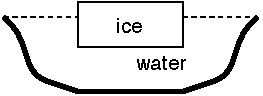
\includegraphics{../../figures/bathtub.pdf}
\caption{Ice in a Bathtub}
\label{f:models-bathtub}
\end{figure}

The correct answer is that the level stays the same:
the ice displaces its own weight in water,
so it exactly fills the ``hole'' it has made when it melts.
Figuring out why helps people build a model of the relationship between weight, volume, and density \cite{Epst2002}.

Describe another formative assessment you have seen or used
that required people to think something through
and thereby identified flaws in their reasoning.
When you are done,
explain your example to a partner
and give them feedback on theirs.

\subsection*{A Different Progression (individual/15)}

The novice-competent-expert model of skill development
is sometimes called the \href{https://en.wikipedia.org/wiki/Dreyfus\_model\_of\_skill\_acquisition}{Dreyfus model}.
Another commonly-used progression is
the \href{https://en.wikipedia.org/wiki/Four\_stages\_of\_competence}{four stages of competence}:

\begin{description}

\item[Unconscious incompetence:]
  the person doesn't know what they don't know.

\item[Conscious incompetence:]
  the person realizes that they don't know something.

\item[Conscious competence:]
  the person has learned how to do something,
  but can only do it while concentrating
  and may still need to break things down into steps.

\item[Unconscious competence:]
  the skill has become second nature
  and the person can do it reflexively.

\end{description}

Identify one subject where you are at each level.
What level are most of your learners at in the subject you teach most often?
What level are you trying to get them to?
How do these four stages relate to the novice-competent-expert classification?

\subsection*{What Kind of Computing? (individual/10)}

\cite{Tedr2008} summarizes three traditions in computing:

\begin{description}

\item[Mathematical:]
  Programs are the embodiment of algorithms.
  They are either correct or incorrect,
  as well as more or less efficient.

\item[Scientific:]
  Programs are more or less accurate models of information processes
  that can be studied using the scientific method.

\item[Engineering:]
  Programs are built objects like dams and airplanes,
  and are more or less effective and reliable.

\end{description}

Which of these best matches your mental model of computing?
If none of them do, what model do you have?

\subsection*{Explaining Why Not (pairs/5)}

One of your learners thinks that there is some kind of difference between
text that they type in character by character
and identical text that they copy and paste.
Think of a reason they might believe this
or something that might have happened to give them this impression,
then pretend to be that learner while your partner explains why this isn't the case.
Trade roles and try again.

\subsection*{Your Model Now (whole class/5)}

As a class,
create a list of the key elements of your mental model of learning.
What are the half-dozen most important concepts and how do they relate?

\subsection*{Your Notional Machines (small groups/20)}

Working in small groups,
write up a description of the notional machine you want learners to use
to understand how their programs run.
How does a notional machine for a blocks-based language like Scratch
differ from that for Python?
What about a notional machine for spreadsheets
or for a browser that is interpreting HTML and CSS when rendering a web page?

\chaplbl{Expertise and Memory}{s:memory}

\begin{quote}

  Memory is the residue of thought. \\
  --- Dan Willingham

\end{quote}

The previous chapter explained the differences between novices and competent practitioners.
This one looks at expertise:
what it is,
how people acquire it,
and how it can be harmful as well as helpful.
We then introduce one of the most important limits on learning
and look at how drawing pictures of mental models can help us turn knowledge into lessons.

To start,
what do we mean when we say someone is an expert?
The usual answer is that they can solve problems much faster than people who are ``merely competent'',
or that they can recognize and deal with cases where the normal rules don't apply.
They also somehow make this look effortless:
in many cases,
they seem to know the right answer at a glance~\cite{Parn2017}.

Expertise is more than just knowing more facts:
competent practitioners can memorize a lot of trivia without noticeably improving their performance.
Instead,
imagine for a moment that we store knowledge as a network or graph
in which facts are nodes
and relationships are arcs\footnote{This is definitely \emph{not} how our brains work, but it's a useful metaphor.}.
The key difference between experts and competent practitioners is that
experts' mental models are much more densely connected,
i.e.,
they are more likely to know a connection between any two facts.

The graph metaphor explains why helping learners make connections
is as important as introducing them to facts:
without those connections,
people can't recall and use what they know.
It also explains many observed aspects of expert behavior:

\begin{itemize}

\item
  Experts can often jump directly from a problem to a solution
  because there actually is a direct link between the two in their mind.
  Where a competent practitioner would have to reason
  $A{\rightarrow}B{\rightarrow}C{\rightarrow}D{\rightarrow}E$,
  an expert can go from $A$ to $E$ in a single step.
  We call this \emph{intuition}:
  instead of reasoning their way to a solution,
  the expert recognizes a solution in the same way that they would recognize a familiar face.

\item
  Densely-connected graphs are also the basis for experts' \gref{g:fluid-representation}{fluid representations},
  i.e.,
  their ability to switch back and forth between different views of a problem~\cite{Petr2016}.
  For example,
  when trying to solve a problem in mathematics,
  an expert might switch between tackling it geometrically
  and representing it as a set of equations.

\item
  This metaphor also explains why experts are better at diagnosis than competent practitioners:
  more linkages between facts makes it easier to reason backward from symptoms to causes.
  (This in turn is why asking programmers to debug during job interviews
  gives a more accurate impression of their ability than asking them to program.)

\item
  Finally,
  experts are often so familiar with their subject that
  they can no longer imagine what it's like to \emph{not} see the world that way.
  This means they are often less good at teaching the subject than people with less expertise
  who still remember learning it themselves.

\end{itemize}

The last of these points is called \gref{g:expert-blind-spot}{expert blind spot}.
As originally defined in~\cite{Nath2003},
it is the tendency of experts to organize explanation according to the subject's deep principles
rather than being guided by what their learners already know.
It can be overcome with training,
but it is part of reason there is no correlation between
how good someone is at doing research in an area
and how good they are at teaching it~\cite{Mars2002}.

\begin{aside}{The J Word}
  Experts often betray their blind spot by using the word ``just'',
  as in,
  ``Oh, it's easy, you just fire up a new virtual machine
  and then you just install these four patches to Ubuntu
  and then you just re-write your entire program in a pure functional language.''
  As we discuss in \chapref{s:motivation},
  doing this signals that the speaker thinks the problem is trivial
  and that the person struggling with it must therefore be stupid,
  so don't do this.
\end{aside}

\seclbl{Concept Maps}{s:memory-concept-maps}

Our tool of choice for representing someone's mental model is a \gref{g:concept-map}{concept map}
in which facts are bubbles and connections are labelled connections.
As examples,
\figref{f:memory-seasons} shows why the Earth has seasons (from \hreffoot{https://cmap.ihmc.us/}{IHMC}),
and \appref{s:conceptmaps} presents concept maps for several key ideas in this book.

\figpdf{figures/seasons.pdf}{Concept Map for Seasons}{f:memory-seasons}

To show how concept maps can be using in teaching programming, consider this \texttt{for} loop in Python:

\begin{minted}{text}
for letter in "abc":
    print(letter)
\end{minted}

\noindent
whose output is:

\begin{minted}{text}
a
b
c
\end{minted}

The three key ``things'' in this loop are shown in the top of \figref{f:memory-loop}, but they are only half the story.
The expanded version in the bottom shows the \emph{relationships} between those things,
which are as important for understanding as the concepts themselves.

\figpdf{figures/for-loop.pdf}{Concept Map for a For Loop}{f:memory-loop}

\newpage
Concept maps can be used in many ways:

\begin{description}

\item[Helping teachers figure out what they're trying to teach.]
  A concept map separates content from order:
  in our experience,
  people rarely wind up teaching things in the order in which they first drew them.

\item[Aiding communication between lesson designers.]
  Teachers with very different ideas of what they're trying to teach
  are likely to pull their learners in different directions.
  Drawing and sharing concept maps can help prevent this.
  And yes,
  different people may have different concept maps for the same topic,
  but concept mapping makes those differences explicit.

\item[Aiding communication with learners.]
  While it's possible to give learners a pre-drawn map at the start of a lesson for them to annotate,
  it's better to draw it piece by piece while teaching
  to reinforce the ties between what's in the map and what the teacher said.
  We will return to this idea in \secref{s:architecture-brain}.

\item[For assessment.]
  Having learners draw pictures of what they think they just learned
  shows the teacher what they missed and what was miscommunicated.
  Reviewing learners' concept maps is too time-consuming to do as a formative assessment during class,
  but very useful in weekly lectures \emph{once learners are familiar with the technique}.
  The qualification is necessary because
  any new way of doing things initially slows people down---if a learner is trying to make sense of basic programming,
  asking them to figure out how to draw their thoughts at the same time is an unfair load.

\end{description}

Some teachers are also skeptical of whether novices can effectively map their understanding,
since introspection and explanation of understanding are generally more advanced skills than understanding itself.
For example,
\cite{Kepp2008} looked at the use of concept mapping in computing education.
One of their findings was that,
``{\ldots}concept mapping is troublesome for many students because
it tests personal understanding rather than knowledge that was merely learned by rote.''
As someone who values understanding over rote knowledge,
I consider that a benefit.

\begin{aside}{Start Anywhere}
  When first asked to draw a concept map, many people will not know where to start.
  When this happens,
  write down two words associated with the topic you're trying to map,
  then draw a line between them and add a label explaining how those two ideas are related.
  You can then ask what other things are related in the same way,
  what parts those things have,
  or what happens before or after the concepts already on the page
  in order to discover more nodes and arcs.
  After that, the hard part is often stopping.
\end{aside}

Concept maps are just one way to represent our understanding of a subject~\cite{Eppl2006};
others include Venn diagrams, flowcharts, and decision trees~\cite{Abel2009}.
All of these \gref{g:externalized-cognition}{externalize cognition},
i.e.,
make mental models visible so that they can be compared and combined\footnote{To paraphrase Oscar Wilde's Lady Windermere,
people often don't know what they're thinking until they've heard themselves say it.}

\begin{aside}{Rough Work and Honesty}
  Many user interface designers believe that
  it's better to show people rough sketches of their ideas rather than polished mock-ups
  because people are more likely to give honest feedback on something that they think
  only took a few minutes to create:
  if it looks as though what they're critiquing took hours to create,
  most will pull their punches.
  When drawing concept maps to motivate discussion,
  you should therefore use pencils and scrap paper (or pens and a whiteboard)
  rather than fancy computer drawing tools.
\end{aside}

\seclbl{Seven Plus or Minus Two}{s:memory-seven-plus-or-minus}

While the graph model of knowledge is wrong but useful,
another simple model has a sounder physiological basis.
As a rough approximation,
human memory can be divided into two distinct layers.
The first,
called \gref{g:long-term-memory}{long-term} or \gref{g:persistent-memory}{persistent memory},
is where we store things like our friends' names,
our home address,
and what the clown did at our eighth birthday party that scared us so much.
Its capacity is essentially unlimited,
but it is slow to access---too slow to help us cope with hungry lions and disgruntled family members.

Evolution has therefore given us a second system
called \gref{g:short-term-memory}{short-term} or \gref{g:working-memory}{working memory}.
It is much faster,
but also much smaller:~\cite{Mill1956} estimated that the average adult's working memory could only hold 7±2 items at a time.
This is why \hreffoot{https://www.quora.com/Why-did-Bell-Labs-create-phone-numbers-of-7-digits-10-digits-Is-there-a-reason-that-dashes-and-brackets-are-used}{phone numbers}
are 7 or 8 digits long:
back when phones had dials instead of keypads,
that was the longest string of numbers most adults could remember accurately for as long as it took the dial to go around several times.

\begin{aside}{Participation}
  The size of working memory is sometimes used to explain
  why sports teams tend to have about half a dozen members
  or are broken into sub-groups like the forwards and backs in rugby.
  It is also used to explain why meetings are only productive up to a certain number of participants:
  if twenty people try to discuss something,
  either three meetings are going on at once
  or half a dozen people are talking while everyone else listens.
  The argument is that people's ability to keep track of their peers is constrained by the size of working memory,
  but so far as I know,
  the link has never been proven.
\end{aside}

7±2 is the single most important number in teaching.
A teacher cannot place information directly in a learner's long-term memory.
Instead,
whatever they present is first stored in the learner's short-term memory,
and is only transferred to long-term memory after it has been held there and rehearsed (\secref{s:individual-strategies}).
If the teacher presents too much information too quickly,
the new information displaces the old
before the latter is transferred.

This is one of the ways to use a concept map when designing a lesson:
it helps make sure learners' short-term memories won't be overloaded.
Once the map is drawn,
the teacher chooses a subsection that fill fit in short term memory
and lead to a formative assessment,
then chooses another subsection and so on (\figref{f:memory-photosynthesis}).

\figpdf{figures/photosynthesis.pdf}{Using Concept Maps in Lesson Design}{f:memory-photosynthesis}

\begin{aside}{Building Concept Maps Together}
  The next time you have a team meeting,
  give everyone a sheet of paper
  and have them spend a few minutes drawing their own concept map of the project you're all working on.
  On the count of three,
  have everyone reveal their concept maps to their group.
  The discussion that follows may help people understand
  why they've been tripping over each other.
\end{aside}

The simple model of memory presented here has largely been replaced by a more sophisticated one
in which short-term memory is broken down into several modal stores
(e.g., for visual vs. linguistic memory),
each of which does some involuntary preprocessing~\cite{Mill2016a}.
Our presentation is therefore an example of a mental model that aids learning and everyday work.

\subsection*{Pattern Recognition}

Recent research suggests that the actual size of short-term memory
might be as low as 4±1 items~\cite{Dida2016}.
In order to handle larger sets of information,
our minds create \gref{g:chunking}{chunks}.
For example,
most of us remember words as single items rather than as sequences of letters.
Similarly,
the pattern made by five spots on cards or dice is remembered as a whole
rather than as five separate pieces of information.

Experts have more and larger chunks than non-experts,
i.e., experts ``see'' larger patterns and have more patterns to match things against.
This allows them to reason at a higher level
and to search for information more quickly and more accurately.
However,
chunking can also mislead us if we mis-identify things:
newcomers really can sometimes see things that experts have looked at and missed.

Given how important chunking is to thinking,
it is tempting to identify \hreffoot{https://en.wikipedia.org/wiki/Software\_design\_pattern}{design patterns}
and teach them directly.
These patterns help competent practitioners think and talk to each other in many domains (including teaching~\cite{Berg2012}),
but pattern catalogs are too dry and too abstract for novices to make sense of on their own.
That said,
giving names to a small number of patterns does seem to help with teaching,
primarily by giving the learners a richer vocabulary to think and communicate with \cite{Kuit2004,Byck2005,Saja2006}.
We will return to this in \secref{s:pck-programming}.

\seclbl{Becoming an Expert}{s:memory-becoming-expert}

So how does someone become an expert?
The idea that ten thousand hours of practice will do it is widely quoted
but \hreffoot{http://www.goodlifeproject.com/podcast/anders-ericsson/}{probably not true}:
doing the same thing over and over again is much more likely to solidify bad habits than improve performance.
What actually works is doing similar but subtly different things,
paying attention to what works and what doesn't,
and then changing behavior in response to that feedback to get cumulatively better.
This is called \gref{g:deliberate-practice}{deliberate}
or \gref{g:reflective-practice}{reflective practice},
and a common progression is for people to go through three stages:

\begin{description}

\item[Act on feedback from others.]
  A learner might write an essay about what they did on their summer holiday
  and get feedback from a teacher telling them how to improve it.

\item[Give feedback on others' work.]
  The learner might critique character development in a Harry Potter novel
  and get feedback from the teacher on their critique.

\item[Give feedback to themselves.]
  At some point,
  the learner starts critiquing their own work as they do it
  using the skills they have now built up.
  Doing this is so much faster than waiting for feedback from others
  that proficiency suddenly starts to take off.

\end{description}

\begin{aside}{What Counts as Deliberate Practice?}
  \cite{Macn2014} found that,
  ``{\ldots}deliberate practice explained 26\% of the variance in performance for games,
  21\% for music,
  18\% for sports,
  4\% for education,
  and less than 1\% for professions.''
  However,~\cite{Eric2016} critiqued this finding by saying,
  ``Summing up every hour of any type of practice during an individual's career
  implies that the impact of all types of practice activity on performance is equal---an assumption
  that{\ldots}is inconsistent with the evidence.''
  To be effective,
  deliberate practice requires both a clear performance goal
  and immediate informative feedback,
  both of which are things teachers should strive for anyway.
\end{aside}

\seclbl{Exercises}{s:memory-exercises}

\exercise{Concept Mapping}{pairs}{30}

Draw a concept map for something you would teach in five minutes.
Trade with a partner and critique each other's maps.
Do they present concepts or surface detail?
Which of the relationships in your partner's map do you consider concepts and vice versa?

\exercise{Concept Mapping (Again)}{small groups}{20}

Working in groups of 3--4,
have each person independently draw a concept map showing their mental model of what goes on in a classroom.
When everyone is done,
compare the concept maps.
Where do your mental models agree and disagree?

\exercise{Enhancing Short-Term Memory}{individual}{5 minutes}

\cite{Cher2007} suggests that
the main reason people draw diagrams when they are discussing things
is to enlarge their short-term memory:
pointing at a wiggly bubble drawn a few minutes ago triggers recall of several minutes of debate.
When you exchanged concept maps in the previous exercise,
how easy was it for other people to understand what your map meant?
How easy would it be for you if you set it aside for a day or two and then looked at it again?

\exercise{That's a Bit Self-Referential, Isn't It?}{whole class}{30}

\begin{enumerate}

\item
  Working independently,
  draw a concept map for concept maps.

\item
  Compare your concept map with those drawn by other people.
  What did most people include?
  What were the significant differences?

\end{enumerate}

\exercise{Noticing Your Blind Spot}{small groups}{10}

Elizabeth Wickes listed
\hreffoot{https://twitter.com/elliewix/status/981285432922202113}{all the things you need to understand}
in order to read this one line of Python:

\begin{minted}{text}
answers = ['tuatara', 'tuataras', 'bus', "lick"]
\end{minted}

\begin{itemize}
\item
  The square brackets surrounding the content mean we're working with a list
  (as opposed to square brackets immediately to the right of something,
  which is a data extraction notation).
\item
  The elements are separated by commas outside and between the quotes
  (rather than inside, as they would be for quoted speech).
\item
  Each element is a character string,
  and we know that because of the quotes.
  We could have number or other data types in here if we wanted;
  we need quotes because we're working with strings.
\item
  We're mixing our use of single and double quotes;
  Python doesn't care so long as they balance around the individual strings.
\item
  Each comma is followed by a space,
  which is not required by Python,
  but which we prefer it for readability.
\end{itemize}

Each of these details might be overlooked by an expert.
Working in groups of 3--4,
select something equally short from a lesson you have recently taught or learned
and break it down to this level of detail.

\exercise{The Power of Chunking}{individual}{5}

Look at \figref{f:memory-unchunked} for 10 seconds,
then look away and try to write out your phone number with these symbols\footnote{
  My thanks to Warren Code for introducing me to this example.
}.
(Use a space for '0'.)
When you are finished,
look at the alternative representation in \appref{s:chunking}.
How much easier are the symbols to remember when the pattern is made explicit?

\figpdfhere{figures/chunking-unchunked.pdf}{Unchunked Representation}{f:memory-unchunked}

\chaplbl{Cognitive Architecture}{s:architecture}

We have been talking about mental models as if they were real things,
but what actually goes on in a learner's brain when they're learning?
The short answer is that we don't know;
the longer answer is that we know a lot more than we used to.
This chapter will dig a little deeper into what brains do while they're learning
and how we can leverage that to design and deliver lessons more effectively.

\seclbl{What's Going On In There?}{s:architecture-brain}

\figpdf{figures/cognitive-architecture.pdf}{Cognitive Architecture}{f:arch-model}

\figref{f:arch-model} is a simplified model of human cognitive architecture.\index{cognitive architecture}
The core of this model is
the separation between short-term and long-term memory discussed in \secref{s:memory-seven-plus-or-minus}.
Long-term memory is like your basement:\index{long-term memory}
it stores things more or less permanently,
but you can't access its contents directly.
Instead,
you rely on your short-term memory,\index{short-term memory}
which is the cluttered kitchen table of your mind.

When you need something,
your brain retrieves it from long-term memory and puts it in short-term memory.
Conversely,
new information that arrives in short-term memory
has to be encoded to be stored in long-term memory.
If that information isn't encoded and stored,
it's not remembered and learning hasn't taken place.

Information gets into short-term memory primarily through
your verbal channel (for speech)\index{channel!verbal}
and visual channel\index{channel!visual}
(for images)\footnote{
  A more complete model
  would also include your senses of touch, smell, and taste,
  but we'll ignore those for now.}.
Most people rely primarily on their visual channel,
but when images and words complement each other,
the brain does a better job of remembering them both:
they are encoded together,
so recall of one later on helps trigger recall of the other.

Linguistic and visual input are processed by different parts of the human brain,
and linguistic and visual memories are stored separately as well.
This means that correlating linguistic and visual streams of information takes cognitive effort:
when someone reads something while hearing it spoken aloud,
their brain can't help but check that it's getting the same information on both channels.

Learning is therefore increased when information is presented simultaneously in two different channels,
but is reduced when that information is redundant rather than complementary,
a phenomenon called the \gref{g:split-attention-effect}{split-attention effect}~\cite{Maye2003}.
For example,
people generally find it harder to learn from a video that has both narration and on-screen captions
than from one that has either the narration or the captions but not both,
because some of their attention has to be devoted to checking
that the narration and the captions agree with each other.
Two notable exceptions to this are people who do not yet speak the language well
and people with hearing impairments or other special needs,
both of whom may find that the value of the redundant information
outweighs the extra processing effort.

\begin{aside}{Piece by Piece}
  The split attention effect explains why
  it's more effective to draw a diagram piece by piece while teaching
  than to present the whole thing at once.
  If parts of the diagram appear at the same time as things are being said,
  the two will be correlated in the learner's memory.
  Pointing at part of the diagram later
  is then more likely to trigger recall of what was being said when that part was being drawn.
\end{aside}

The split-attention effect does \emph{not} mean
that learners shouldn't try to reconcile multiple incoming streams of information---after all,
this is what they have to do in the real world~\cite{Atki2000}.
Instead,
it means that instruction shouldn't require people to do it
while they are first mastering unit skills;
instead,
using multiple sources of information simultaneously should be treated as a separate learning task.

\begin{aside}{Not All Graphics Are Created Equal}
  \cite{Sung2012} presents an elegant study that distinguishes \emph{seductive} graphics\index{graphics!seductive}
  (which are highly interesting but not directly relevant to the instructional goal),
  \emph{decorative} graphics\index{graphics!decorative}
  (which are neutral but not directly relevant to the instructional goal),
  and \emph{instructive} graphics\index{graphics!instructive}
  (which are directly relevant to the instructional goal).
  Learners who received any kind of graphic gave material higher satisfaction ratings
  than those who didn't get graphics,
  but only learners who got instructive graphics actually performed better.

  Similarly,~\cite{Stam2013,Stam2014} found that
  having more information can actually lower performance.
  They showed children pictures, pictures and numbers, or just numbers for two tasks.
  For some,
  having pictures or pictures and numbers outperformed having numbers only,
  but for others,
  having pictures outperformed pictures and numbers,
  which outperformed just having numbers.
\end{aside}

\seclbl{Cognitive Load}{s:architecture-load}

In~\cite{Kirs2006}, Kirschner, Sweller and Clark wrote:

\begin{quote}

  Although unguided or minimally guided instructional approaches
  are very popular and intuitively appealing{\ldots}these approaches ignore
  both the structures that constitute human cognitive architecture
  and evidence from empirical studies over the past half-century
  that consistently indicate that minimally guided instruction is less effective and less efficient
  than instructional approaches that place a strong emphasis on guidance of the student learning process.
  The advantage of guidance begins to recede
  only when learners have sufficiently high prior knowledge to provide ``internal'' guidance.

\end{quote}

Beneath the jargon,
the authors were claiming that having learners ask their own questions,
set their own goals,
and find their own path through a subject
is less effective than showing them how to do things step by step.
The ``choose your own adventure'' approach is known as \gref{g:inquiry-based-learning}{inquiry-based learning},
and is intuitively appealing:
after all,
who would argue \emph{against} having learners use their own initiative
to solve real-world problems in realistic ways?
However,
asking learners to do this in a new domain overloads them
by requiring them to master a domain's factual content
and its problem-solving strategies
at the same time.

More specifically,
\gref{g:cognitive-load}{cognitive load theory} proposed that
people have to deal with three things when they're learning:

\begin{description}

\item[\grefdex{g:intrinsic-load}{Intrinsic load}{cognitive load!intrinsic}]
  is what people have to keep in mind in order to absorb new material.

\item[\grefdex{g:germane-load}{Germane Load}{cognitive load!germane}]
  is the (desirable) mental effort required to link new information to old,
  which is one of the things that distinguishes learning from memorization.

\item[\grefdex{g:extraneous-load}{Extraneous Load}{cognitive load!extraneous}]
  is anything that distracts from learning.

\end{description}

Cognitive load theory holds that
people have to divide a fixed amount of working memory between these three things.
Our goal as teachers is to maximize the memory available to handle intrinsic load,
which means reducing the germane load at each step and eliminating the extraneous load.

\subsection*{Parsons Problems}

One kind of exercise that can be explained in terms of cognitive load
is often used when teaching languages.
Suppose you ask someone to translate the sentence, ``How is her knee today?'' into Frisian.
To solve the problem,
they need to recall both vocabulary and grammar,
which is a double cognitive load.
If you ask them to put ``hoe'', ``har'', ``is'', ``hjoed'', and ``knie'' in the right order,
on the other hand,
you are allowing them to focus solely on learning grammar.
If you write these words in five different fonts or colors,
though,
you have increased the extraneous cognitive load,
because they will involuntarily (and possibly unconsciously) expend some effort
trying to figure out if the differences are meaningful
(\figref{f:architecture-frisian}).

\figimg{figures/frisian.png}{Constructing a Sentence}{f:architecture-frisian}

The coding equivalent of this
is called a \gref{g:parsons-problem}{Parsons Problem}\footnote{Named after one of its creators.}~\cite{Pars2006}.
When teaching people to program,
you can give them the lines of code they need to solve a problem
and ask them to put them in the right order.
This allows them to concentrate on control flow and data dependencies
without being distracted by variable naming or trying to remember what functions to call.
Multiple studies have shown that Parsons Problems take less time for learners to do
but produce equivalent educational outcomes~\cite{Eric2017}.

\subsection*{Faded Examples}

Another type of exercise that can be explained in terms of cognitive load
is to give learners a series of \grefdex{g:faded-example}{faded examples}{faded example}.
The first example in a series presents a complete use of a particular problem-solving strategy.
The next problem is of the same type,
but has some gaps for the learner to fill in.
Each successive problem gives the learner less \gref{g:scaffolding}{scaffolding},
until they are asked to solve a complete problem from scratch.
When teaching high school algebra,
for example,
we might start with this:

\begin{center}
\begin{tabular}{rcl}
  (4x + 8)/2	& = &	5	\\
  4x + 8	& = &	2 * 5	\\
  4x + 8	& = &	10	\\
  4x		& = &	10 - 8	\\
  4x		& = &	2	\\
  x		& = &	2 / 4	\\
  x		& = &	1 / 2
\end{tabular}
\end{center}

\noindent
and then ask learners to solve this:

\begin{center}
\begin{tabular}{rcl}
  (3x - 1)*3	& = &	12	\\
  3x - 1	& = &	\_ / \_	\\
  3x - 1	& = &	4	\\
  3x		& = &	\_	\\
  x		& = &	\_ / 3	\\
  x		& = &	\_
\end{tabular}
\end{center}

\noindent
and this:

\begin{center}
\begin{tabular}{rcl}
  (5x + 1)*3	& = &	4	\\
  5x + 1	& = &	\_ 	\\
  5x		& = &	\_ 	\\
  x		& = &	\_
\end{tabular}
\end{center}

\noindent
and finally this:

\begin{center}
\begin{tabular}{rcl}
  (2x + 8)/4	& = &	1	\\
   x		& = &	\_
\end{tabular}
\end{center}

A similar exercise for teaching programming might start by showing learners
how to find the total length of a list of words:

\begin{minted}{text}
# total_length(["red", "green", "blue"]) => 12
define total_length(list_of_words):
    total = 0
    for word in list_of_words:
        total = total + length(word)
    return total
\end{minted}

\noindent
and then ask them to fill in the blanks in this
(which focuses their attention on control structures):

\begin{minted}{text}
# word_lengths(["red", "green", "blue"]) => [3, 5, 4]
define word_lengths(list_of_words):
    list_of_lengths = []
    for ____ in ____:
        append(list_of_lengths, ____)
    return list_of_lengths
\end{minted}

The next problem might be this
(which focuses their attention on updating the final result):

\begin{minted}{text}
# join_all(["red", "green", "blue"]) => "redgreenblue"
define join_all(list_of_words):
    joined_words = ____
    for ____ in ____:
        ____
    return joined_words
\end{minted}

Learners would finally be asked to write an entire function on their own:

\begin{minted}{text}
# make_acronym(["red", "green", "blue"]) => "RGB"
define make_acronym(list_of_words):
    ____
\end{minted}

Faded examples work because
they introduce the problem-solving strategy piece by piece:
at each step,
learners have one new problem to tackle,
which is less intimidating than a blank screen or a blank sheet of paper (\secref{s:classroom-practices}).
It also encourages learners to think about the similarities and differences between various approaches,
which helps create the linkages in their mental models that help retrieval.

The key to constructing a good faded example is
to think about the problem-solving strategy it is meant to teach.
For example,
the programming problems above all use the accumulator design pattern,
in which the results of processing items from a collection
are repeatedly added to a single variable in some way to create the final result.

\begin{aside}{Cognitive Apprenticeship}
  An alternative model of learning and instruction that also uses scaffolding and fading
  is \gref{g:cognitive-apprenticeship}{cognitive apprenticeship},
  which emphasizes the way in which a master passes on skills and insights to an apprentice.
  The master provides models of performance and outcomes,
  then coaches novices by explaining what they are doing and why~\cite{Coll1991,Casp2007}.
  The apprentice reflects on their own problem solving,
  e.g.,
  by thinking aloud or critiquing their own work,
  and eventually explores problems of their own choosing.

  This model tells us that
  teachers should present several examples when presenting a new idea
  so that learners can see what to generalize,
  and that we should vary the form of the problem to make it clear
  what are and aren't superficial features\footnote{For a long time,
    I believed that the variable holding the value a function was going to return
    \emph{had} to be called \texttt{result}
    because my teacher always used that name in examples.}.
  Problems should be presented in real-world contexts,
  and we should encourage self-explanation to help learners organize and make sense of what they have just been taught
  (\secref{s:individual-strategies}).
\end{aside}

\subsection*{Labelled Subgoals}

\grefdex{g:subgoal-labelling}{Labelling subgoals}{labelled subgoals} means
giving names to the steps in a step-by-step description of a problem-solving process.
\cite{Marg2016,Morr2016} found that learners with labelled subgoals
solved Parsons Problems better than learners without,
and the same benefit is seen in other domains~\cite{Marg2012}.
Returning to the Python example used earlier,
the subgoals in finding the total length of a list of words or constructing an acronym are:

\begin{enumerate}

\item
  Create an empty value of the type to be returned.

\item
  Get the value to be added to the result from the loop variable.

\item
  Update the result with that value.

\end{enumerate}

Labelling subgoals works because grouping related steps into named chunks (\secref{s:memory-seven-plus-or-minus})\index{chunking}
helps learners distinguish what's generic from what is specific to the problem at hand.
It also helps them build a mental model of that kind of problem
so that they can solve other problems of that kind,
and gives them a natural opportunity for self-explanation (\secref{s:individual-strategies}).

\subsection*{Minimal Manuals}

The purest application of cognitive load theory may be John Carroll's\index{Carroll, John}
\gref{g:minimal-manual}{minimal manual}~\cite{Carr1987,Carr2014}.
Its starting point is a quote from a user:
``I want to do something, not learn how to do everything.''
Carroll and colleagues redesigned training to present every idea as a single-page self-contained task:
a title describing what the page was about,
step-by-step instructions of how to do just one thing
(e.g., how to delete a blank line in a text editor),
and then several notes how to recognize and debug common problems.
They found that rewriting training materials this way made them shorter overall,
and that people using them learned faster.
Later studies confirmed that this approach outperformed the traditional approach
regardless of prior experience with computers~\cite{Lazo1993}.
\cite{Carr2014} summarized this work by saying:

\begin{quote}

  Our ``minimalist'' designs sought to leverage user initiative and prior knowledge,
  instead of controlling it through warnings and ordered steps.
  It emphasized that users typically bring much expertise and insight to this learning,
  for example,
  knowledge about the task domain,
  and that such knowledge could be a resource to instructional designers.
  Minimalism leveraged episodes of error recognition, diagnosis, and recovery,
  instead of attempting to merely forestall error.
  It framed troubleshooting and recovery as learning opportunities instead of as aberrations.

\end{quote}

\seclbl{Other Models of Learning}{s:architecture-theory}

Critics of cognitive load theory have sometimes argued that\index{cognitive load!criticism of}
any result can be justified after the fact by labelling things that hurt performance as extraneous load
and things that don't as intrinsic or germane.
However,
instruction based on cognitive load theory is undeniably effective.
For example,
\cite{Maso2016} redesigned a database course to remove split attention and redundancy effects
and to provide worked examples and sub-goals.
The new course reduced the exam failure rate by 34\%
and increased learner satisfaction.

A decade after the publication of~\cite{Kirs2006},
a growing number of people believe that cognitive load theory and inquiry-based approaches are compatible
if viewed in the right way.
\cite{Kaly2015} argues that cognitive load theory is basically micro-management of learning
within a broader context that considers things like motivation,
while~\cite{Kirs2018} extends cognitive load theory to include collaborative aspects of learning.
As with~\cite{Mark2018} (discussed in \secref{s:individual-strategies}),
researchers' perspectives may differ,
but the practical implementation of their theories often wind up being the same.

One of the challenges in educational research is that
what we mean by ``learning'' turns out to be complicated
once you look beyond the standardized Western classroom.
Two specific perspectives from \gref{g:educational-psychology}{educational psychology} have influenced this book.
The one we have used so far is \gref{g:cognitivism}{cognitivism},
which focuses on things like pattern recognition, memory formation, and recall.
It is good at answering low-level questions,
but generally ignores larger issues like,
``What do we mean by `learning'?''
and, ``Who gets to decide?''
The other is \gref{g:situated-learning}{situated learning},
which focuses on bringing people into a community
and recognizes that
teaching and learning are always rooted in who we are and who we aspire to be.
We will discuss it in more detail in \chapref{s:community}.

The \hreffoot{http://www.learning-theories.com/}{Learning Theories website}
and~\cite{Wibu2016}
have good summaries of these and other perspectives.
Besides cognitivism,
those encountered most frequently include \gref{g:behaviorism}{behaviorism}
(which treats education as stimulus/response conditioning),
\gref{g:constructivism}{constructivism}
(which considers learning an active process during which learners construct knowledge for themselves),
and \gref{g:connectivism}{connectivism}
(which holds that knowledge is distributed,
that learning is the process of navigating, growing, and pruning connections,
and which emphasizes the social aspects of learning made possible by the Internet).
These perspectives can help us organize our thoughts,
but in practice,
we always have to try new methods in the class,
with actual learners,
in order to find out how well they balance the many forces in play.

\seclbl{Exercises}{s:architecture-exercises}

\exercise{Create a Faded Example}{pairs}{30}

It's very common for programs to count how many things fall into different categories:
for example,
how many times different colors appear in an image,
or how many times different words appear in a paragraph of text.

\begin{enumerate}
\item
  Create a short example (no more than 10 lines of code) that shows people how to do this,
  and then create a second example that solves a similar problem in a similar way
  but has a couple of blanks for learners to fill in.
  How did you decide what to fade out?
  What would the next example in the series be?

\item
  Define the audience for your examples.
  For example,
  are these beginners who only know some basics programming concepts?
  Or are these learners with some experience in programming?

\item
  Show your example to a partner,
  but do \emph{not} tell them what level you think it is for.
  Once they have filled in the blanks,
  ask them to guess the intended level.

\end{enumerate}

If there are people among the trainees who don't program at all,
try to place them in different groups
and have them play the part of learners for those groups.
Alternatively,
choose a different problem domain and develop a faded example for it.

\exercise{Classifying Load}{small groups}{15}

\begin{enumerate}

\item
  Choose a short lesson that a member of your group has taught or taken recently.

\item
  Make a point-form list of the ideas, instructions, and explanations it contains.

\item
  Classify each as intrinsic, germane, or extraneous.
  What did you all agree on?
  Where did you disagree and why?

\end{enumerate}

(The exercise ``Noticing Your Blind Spot'' in \secref{s:memory-exercises}
will give you an idea of how detailed your point-form list should be.)

\exercise{Create a Parsons Problem}{pairs}{20}

Write five or six lines of code that does something useful,
jumble them,
and ask your partner to put them in order.
If you are using an indentation-based language like Python,
do not indent any of the lines;
if you are using a curly-brace language like Java,
do not include any of the curly braces.
(If your group includes people who aren't programmers,
use a different problem domain,
such as making banana bread.)

\exercise{Minimal Manuals}{individual}{20}

Write a one-page guide to doing something that your learners might encounter in one of your classes,
such as centering text horizontally
or printing a number with a certain number of digits after the decimal point.
Try to list at least three or four incorrect behaviors or outcomes the learner might see
and include a one- or two-line explanation
of why each happens and how to correct it.

\exercise{Cognitive Apprenticeship}{pairs}{15}

Pick a coding problem that you can do in two or three minutes
and think aloud as you work through it
while your partner asks questions about what you're doing and why.
Do not just explain what you're doing,
but also why you're doing it,
how you know it's the right thing to do,
and what alternatives you've considered but discarded.
When you are done,
swap roles with your partner and repeat the exercise.

\exercise{Worked Examples}{pairs}{15}

Seeing worked examples helps people learn to program faster than just writing lots of code~\cite{Skud2014},
and deconstructing code by tracing it or debugging it also increases learning~\cite{Grif2016}.
Working in pairs,
go through a 10--15 line piece of code and explain what every statement does
and why it is necessary.
How long does it take?
How many things do you feel you need to explain per line of code?

\exercise{Critiquing Graphics}{individual}{30}

\cite{Maye2009,Mill2016a} presents six principles for good teaching graphics:

\begin{description}

\item[Signalling:]
  visually highlight the most important points
  so that they stand out from less-critical material.

\item[Spatial contiguity:]
  place captions as close to the graphics as practical to offset the cost of shifting between the two.

\item[Temporal contiguity:]
  present spoken narration and graphics as close in time as practical.
  (Presenting both at once is better than presenting them one after another.)

\item[Segmenting:]
  when presenting a long sequence of material or when learners are inexperienced with the subject,
  break the presentation into short segments
  and let learners control how quickly they advance from to the next.

\item[Pre-training:]
  if learners don't know the major concepts and terminology used in your presentation,
  teach just those concepts and terms beforehand.

\item[Modality:]
  people learn better from pictures plus narration than from pictures plus text,
  unless they are non-native speakers
  or there are technical words or symbols.

\end{description}

Choose a video of a lesson or talk online that uses slides or other static presentations
and rate its graphics as ``poor'', ``average'', or ``good'' according to these six criteria.

\section*{Review}

\figpdfhere{figures/conceptmap-cognitive-load.pdf}{Concepts: Cognitive Load}{f:architecture-cognitive-load}

\chaplbl{Individual Learning}{s:individual}

The previous three chapters have looked at what instructors can do to
help their learners. This chapter looks at what learners can do for
themselves by changing their study strategies and getting enough rest.

The key to getting more out of learning is
\gref{g:metacognition}{metacognition}, or thinking about one's
own thinking processes. Just as good musicians listen to their own
playing, and good teachers reflect on their teaching
(Chapter~\ref{s:performance}), learners will learn better and faster if
they make plans, set goals, and monitor their progress. It's difficult
for learners to master these skills in the abstract---for example, just
telling them to make plans doesn't have any effect---but lessons can be
designed to encourage certain study practices, and drawing attention to
these practices in class helps them realize that learning is a skill
that can be improved like any other \cite{McGu2015,Miya2018}.

The big prize is transfer of learning, which occurs when one thing we
have learned helps us learn something else more quickly. Researchers
distinguish between \gref{g:near-transfer}{near transfer}, which occurs
between similar or related areas like fractions and decimals, or loops
in different programming languages, and \gref{g:far-transfer}{far
transfer}, which occurs between dissimilar
domains---the idea that learning to play chess will help mathematical
reasoning or vice versa.

Near transfer undoubtedly occurs---no kind of learning beyond simple
memorization could occur if it didn't---and instructors leverage it all
the time by giving learners exercises that are close in form or content
to what has just been presented in a lesson. However, \cite{Sala2017}
recently analyzed many studies of far transfer and concluded that while
we might \emph{want} to believe in it:

\begin{quote}

{\ldots}the results show small to moderate effects. However, the
effect sizes are inversely related to the quality of the experimental
design{\ldots} We conclude that far transfer of learning rarely
occurs.

\end{quote}

When far transfer \emph{does} occur, it seems to happen only once a subject
has been mastered \cite{Gick1987}. In practice, this means that
learning to program won't help you play chess and vice versa.

\seclbl{Six Strategies}{s:individual-strategies}

Psychologists study learning in a wide variety of ways, but have
reached similar conclusions about what actually works
\cite{Mark2018}. The \hreffoot{http://www.learningscientists.org/}{Learning Scientists}
have catalogued six of these strategies and summarized them in \hreffoot{http://www.learningscientists.org/downloadable-materials}{a set
of downloadable posters}. Teaching
these strategies to students, and mentioning them by name when you use
them in class, can help them learn how to learn faster and better
\cite{Wein2018a}.

\subsection*{Spaced Practice}

Ten hours of study spread out over five days is more effective than two
five-hour days, and far better than one ten-hour day. You should
therefore create a study schedule that spreads study activities over
time: block off at least half an hour to study each topic each day
rather than trying to cram everything in the night before an exam
\cite{Kang2016}.

You should also review material after each class (but not immediately
after---take at least a half-hour break). When reviewing, be sure to
include at least a little bit of older material: for example, spend 20
minutes looking over notes from that day's class, and then 5 minutes
each looking over material from the previous day and from a week before.
(Doing this also helps you catch any gaps or mistakes in previous sets
of notes while there's still time to correct them or ask questions: it's
painful to realize the night before the exam that you have no idea why
you underlined ``Demodulate!!'' three times.)

When reviewing, make notes about things that you had forgotten: for
example, make a flash card for each fact that you couldn't remember, or
that you remembered incorrectly. This will help you focus the next round
of study on things that most need attention.

\begin{aside}{The Value of Lectures}
  According to \cite{Mill2016a}, ``The lectures that predominate in
  face-to-face courses are relatively ineffective ways to teach, but
  they probably contribute to spacing material over time, because they
  unfold in a set schedule over time. In contrast, depending on how the
  courses are set up, online students can sometimes avoid exposure to
  material altogether until an assignment is nigh.''
\end{aside}

\subsection*{Retrieval Practice}

Researchers now believe that the limiting factor for long-term memory is
not retention (what is stored), but recall (what can be accessed).
Recall of specific information improves with practice, so outcomes in
real situations can be improved by taking practice tests or summarizing
the details of a topic from memory and then checking what was and wasn't
remembered. For example, \cite{Karp2008} found that repeated testing
improved recall of word lists from 35\% to 80\%.

Research also shows that recall is better when practice uses
activities similar to those used in testing; for example, writing
personal journal entries helps with multiple-choice quizzes, but less
than doing multiple-choice quizzes \cite{Mill2016a}. This is
called \gref{g:transfer-appropriate-processing}{transfer-appropriate
processing}.

One way to exercise retrieval skills is to solve problems twice. The
first time, do it entirely from memory without notes or discussion with
peers. After grading your own work against a rubric supplied by the
instructor, solve the problem again using whatever resources you want.
The difference between the two shows you how well you were able to
retrieve and apply knowledge.

Another method (mentioned above) is to create flash cards. In physical
form, a question or other prompt is written on one side, and the answer
is written on the other; in digital form, these are ideal for deployment
on mobile devices like phones. If you are studying as part of a group,
you can exchange flash cards with a partner; this also helps you
discover important ideas that you may have missed or misunderstood.

A quicker version of this is
\gref{g:read-cover-retrieve}{read-cover-retrieve}: as you read something,
cover up key terms or sections with small sticky notes. When you are
done, go through it a second time and see how well you can guess
what's under each of those stickies.

Whatever method you use, don't just practice recalling facts and
definitions: make sure you also check your understanding of big ideas
and the connections between them. Sketching a concept map and then
comparing it to your notes or to a previously-drawn concept map is a
quick way to do this.

\begin{aside}{Hypercorrection}
  One powerful finding in learning research is the \gref{g:hypercorrection}{hypercorrection
    effect} \cite{Metc2016}. Most people don't
  like to be told they're wrong, so it's reasonable to assume that the
  more confident someone is that the answer they've given in a test is
  correct, the harder it is to change their mind if they were actually
  wrong. However, it turns out that the opposite is true: the more
  confident someone is that they were right, the more likely they are
  not to repeat the error if they are corrected.
\end{aside}

\subsection*{Interleaving}

One way you can space your practice is to interleave study of different
topics: instead of mastering one subject, then the next, then a third,
shuffle study sessions. Even better, switch up the order: A-B-C-B-A-C is
better than A-B-C-A-B-C, which in turn is better than A-A-B-B-C-C
\cite{Rohrer2015}. This is effective because interleaving fosters
creation of more links between different topics, which in turn increases
retention and recall.

How long you should spend on each item depends on the subject and how
well you know it, but somewhere between 10 and 30 minutes is long enough
for you to get into a state of flow (Section~\ref{s:individual-time}) but
not for your mind to wander. Interleaving study will initially feel
harder than focusing on one topic at a time, but that's a sign that it's
working. If you are making flash cards for yourself, or doing practice
tests, you should see improvement after only a couple of days.

\subsection*{Elaboration}

Explaining things to yourself as you go through them helps you
understand and remember them. One way to do this is to follow up each
answer on a practice quiz with an explanation of why that answer is
correct, or conversely with an explanation of why some other plausible
answer isn't. Another is to tell yourself how a new idea is similar to
or different from one that you have seen previously.

Talking to yourself may seem like an odd way to study, but
\cite{Biel1995} explicitly trained people in self-explanation, and
yes, they outperformed those who hadn't been trained. An exercise that
builds on this is to go through code line by line with a group, having a
different person to explain each line in turn and say why it is there
and what it accomplishes.

\cite{Chi1989} found that some learners simply halt when they hit an
unexplained step (or a step whose explanation they don't understand)
when doing mechanics problems in a physics class. Others who pause their
``execution'' of the example to generate an explanation of what's going on
learn faster. Instructors should therefore demonstrate the latter
strategy to learners.

Explaining things to others even works on exams, though the extent of
the benefits are still being
studied. \cite{Cao2017a,Cao2017b} looked at two-stage
exams, i.e., a normal (individual) exam which is then immediately
followed by a second exam in which students work in small groups to
solve a set of problems. They found significant short-term gains for
students doing exams collaboratively, but not long-term gains, i.e.,
the benefits visible a couple of weeks after the mid-term had faded by
the final. They also found that students in the middle of the class
benefited strongly, and that homogeneous-ability groups benefited,
while heterogeneous groups did not.

\subsection*{Concrete Examples}

One specific form of elaboration is so useful that it deserves its own
heading, and that is the use of concrete examples. Whenever you have a
statement of a general principle, try to provide one or more examples of
its use, or conversely take each particular problem and list the general
principles it embodies. \cite{Raws2014} found that interleaving
examples and definitions made it more likely that learners would
remember the latter correctly.

One structured way to do this is the \hreffoot{https://betterexplained.com/articles/adept-method/}{ADEPT method}: give an
\textbf{A}nalogy, draw a \textbf{D}iagram, present an \textbf{E}xample, describe the
idea in \textbf{P}lain language, and then give the \textbf{T}echnical details.
Again, if you are studying with a partner or in a group, you can swap
and check work: see if you agree that other people's examples actually
embody the principle being discussed, or which principles are used in
an example that they haven't listed.

Another useful technique is to teach by contrast, i.e., to show learners
what a solution is \emph{not}, or what kind of problem a technique \emph{won't}
solve. For example, when showing children how to simplify fractions,
it's important to give them a few like 5/7 that can't be simplified so
that they don't become frustrated looking for answers that don't exist.

\subsection*{Dual Coding}

The last of the six core strategies that the \hreffoot{http://www.learningscientists.org/}{Learning
Scientists} describe is to present words and
images together. As discussed in Section~\ref{s:load-split-attention},
different subsystems in our brains handle and store linguistic and
visual information, and if complementary information is presented
through both channels, then they can reinforce one another. However,
learning is more effective when the same information is \emph{not}
presented simultaneously in two different channels
\cite{Maye2003}, because then the brain has to expend effort to
check the channels against each other.

One way to take advantage of dual coding is to draw or label timelines,
maps, family trees, or whatever else seems appropriate to the material.
(I am personally fond of pictures showing which functions call which
other functions in a program.) Drawing a diagram \emph{without} labels, then
coming back later to label it, is excellent retrieval practice.

\seclbl{Time Management}{s:individual-time}

I used to brag about the hours I was working. Not in so many words, of
course---I had \emph{some} social skills---but I would show up for class around
noon, unshaven and yawning, and casually mention how I'd been up working
`til 6:00 a.m.

Looking back, I can't remember who I was trying to impress. Instead,
what I remember is how much of the work I did in those all-nighters I
threw away once I'd had some sleep, and how much damage the stuff I
didn't throw away did to my grades.

My mistake was to confuse ``working'' with ``being productive''. You can't
produce software (or anything else) without doing some work, but you can
easily do lots of work without producing anything of value. Convincing
people of this can be hard, especially when they're in their teens or
twenties, but pays tremendous dividends.

Scientific study of overwork and sleep deprivation goes back to at least
the 1890s (see \cite{Robi2005} for a short, readable summary). The
most important results for learners are:

\begin{enumerate}
\item
  Working more than eight hours a day for an extended period of time
  lowers your total productivity, not just your hourly
  productivity---i.e., you get less done in total (not just per hour)
  when you're in crunch mode than you do when you work regular hours.
\item
  Working over 21 hours in a stretch increases the odds of you making
  a catastrophic error just as much as being legally drunk.
\item
  Productivity varies over the course of the workday, with the
  greatest productivity occurring in the first four to six hours.
  After enough hours, productivity approaches zero; eventually it
  becomes negative.
\end{enumerate}

These facts have been reproduced and verified for over a century, and
the data behind them is as solid as the data linking smoking to lung
cancer. The catch is that \emph{people usually don't notice their abilities
declining}. Just like drunks who think they're still able to drive,
people who are deprived of sleep don't realize that they're not
finishing their sentences (or thoughts). Five eight-hour days per week
has been proven to maximize long-term total output in every industry
that has ever been studied; studying or programming are no different.

But what about short bursts now and then, like pulling an all-nighter to
meet a deadline? That has been studied too, and the results aren't
pleasant. Your ability to think drops by 25\% for each 24 hours you're
awake. Put it another way, the average person's IQ is only 75 after one
all-nighter, which puts them in the bottom 5\% of the population. Two all
nighters in a row, and their effective IQ is 50, which is the level at
which people are usually judged incapable of independent living.

\begin{aside}{When You Just Can't Say No}
  Research has shown that our ability to exert willpower runs out,
  just like our ability to use muscles: if we have to resist eating
  the last donut on the tray when we're hungry, we are less likely to
  fold laundry and vice versa. This is called \gref{g:ego-depletion}{ego
    depletion} \cite{Mill2016a}, and an effective
  counter is to build up habits so that doing the right thing is
  automatic.
\end{aside}

``But---but---we have so many assignments to do!'', your learners say. ``And
they're all due at once! We \emph{have} to work extra hours to get them all
done!'' No: in order to be productive, they have to prioritize and
focus, and in order to do that, they have to be taught how. One
widely-used technique is to make a list of things that need to be done,
sort them by priority, and then switch off email and other interruptions
for 30-60 minutes and complete one of those tasks. If any task on a
to-do list is more than an hour long, break it down into smaller pieces
and prioritize those separately.

The most important part of this is switching off
interruptions. Despite what many people want to believe, people are
not good at multi-tasking. What we can become good at is
\gref{g:automaticity}{automaticity}, which is the ability to do something
routine in the background while doing something else
\cite{Mill2016a}. Most of us can talk while chopping onions, or
drink coffee while reading; with practice, we can also take notes
while listening, but we can't study effectively, program, or do other
mentally challenging tasks while paying attention to something else.

The point of all this organization and preparation is to get into the
most productive mental state possible. Psychologists call it
\gref{g:flow}{flow} \cite{Csik2008}; athletes call it ``being in the
zone'', while musicians talk about losing themselves in what they're
playing. Whatever name you use, people produce much more per unit of
time in this state than normal.

That's the good news. The bad news is that it takes roughly ten minutes
to get back into a state of flow after an interruption, no matter how
short the interruption was. This means that if you are interrupted half
a dozen times per hour, you are \emph{never} at your productive peak.

\seclbl{Peer Assessment}{s:individual-peer}

Asking people on a team to rate their peers is a common practice in
industry. \cite{Sond2012} surveyed the literature on student peer
assessment, distinguishing between grading and reviewing. The benefits
they found included increasing the amount, diversity, and timeliness of
feedback, helping students exercise higher-level thinking, encouraging
reflective practice, and supporting development of social skills. The
concerns were predictable: validity and reliability, motivation and
procrastination, trolls, collusion, and plagiarism. However, while these
concerns are legitimate, the evidence shows that they aren't significant
in class. For example, \cite{Kauf2000} compared confidential peer
ratings and grades on several axes for two undergraduate engineering
courses and found that self-rating and peer ratings statistically
agreed, that collusion (i.e., everyone giving their peers the same
grades) wasn't significant, that students didn't inflate their
self-ratings, and crucially, that ratings were not biased by gender or
race.

One important variation on peer assessment and review is \gref{g:contributing-student}{contributing
student pedagogy}, in which students produce
artifacts to contribute to other students' learning. This can be
developing a short lesson and sharing it with the class, adding to a
question bank, or writing up notes from a particular lecture for
in-class publication. For example, \cite{Fran2018} found that
students who made short videos to teach concepts to their peers had a
significant increase in their own learning compared to those who only
studied the material or viewed the videos.

Another is \gref{g:calibrated-peer-review}{calibrated peer review}, in
which a student reviews one or more examples using a rubric and
compares their evaluation against the instructor's review of the same
work \cite{Kulk2013}. Only once student's evaluations are close
enough to the instructor's are they allowed to start evaluating peers'
actual work.

As long as evaluation is based on observables, rather than personality
traits, peer assessment can actually be as accurate as assessment by TAs
and other outsiders. ``Observables'' means that instead of asking, ``Is the
person outgoing,'' or ``Does the person have a positive attitude,''
assessments should ask, ``Does the person listen attentively during
meetings,'' or, ``Does the person attempt to solve problems before asking
for help.'' The evaluation form in Section~\ref{s:checklists-teameval} shows a
sample to get you started. To use it, rank yourself and each of your
teammates, then calculate and compare scores.

\seclbl{Exercises}{s:individual-exercises}

\subsection*{Learning Strategies (individual/20)}

\begin{enumerate}
\item
  Which of the six learning strategies do you regularly use? Which
  ones do you not?
\item
  Write down three general concepts that you want your learners to
  master, and then give two specific examples of each. (This uses the
  ``concrete examples'' practice).
\item
  For each of those concepts, work backward from one of your examples
  to explain how the concept explains it. (This uses the ``elaboration''
  practice).
\end{enumerate}

\subsection*{Connecting Ideas (pairs/5)}

This exercise is an example of using elaboration to improve
retention. Pick a partner, and have each person independently choose an
idea, then announce your ideas and try to find a four-link chain that
leads from one to the other. For example, if the two ideas are
``Saskatchewan'' and ``statistics'', the links might be:

\begin{itemize}
\item
  Saskatchewan is a province of Canada;
\item
  Canada is a country;
\item
  countries have governments;
\item
  governments are elected; and
\item
  people try to predict election results using statistics
\end{itemize}

\subsection*{Convergent Evolution (pairs/15)}

One practice that wasn't covered above is \gref{g:guided-notes}{guided
notes}, which are instructor-prepared notes that cue
students to respond to key information in a lecture or discussion. The
cues can be blank spaces where students add information, asterisks
next to terms students should define, etc.

Create 2--4 guided note cards for a lesson you have recently taught or
are going to teach. Swap cards with your partner: how easy is it to
understand what is being asked for? How long would it take to fill in
the prompts?

\subsection*{Changing Minds (pairs/10)}

\cite{Kirs2013} argues that myths about digital natives, learning
styles, and self-educators are all reflections of the mistaken belief
that learners know what is best for them, and cautions that we may be in
a downward spiral in which every attempt by education researchers to
rebut these myths confirms their opponents' belief that learning science
is pseudo-science. Pick one thing you have learned about learning so far
in this book that surprised you or contradicted something you previously
believed, and practice explaining it to a partner in 1--2 minutes. How
convincing are you?

\subsection*{Flash Cards (individual/15)}

Use sticky notes or anything else you have at hand to make up a dozen
flash cards for a topic you have recently taught or learned, trade with
a partner, and see how long it takes each of you to achieve 100\% perfect
recall. When you are done, set the cards aside, then come back after an
hour and see what your recall rate is.

\subsection*{Using ADEPT (whole class/15)}

Pick something you have recently taught or been taught and outline a
short lesson that uses the five-step ADEPT method to introduce it.

\subsection*{The Cost of Multi-Tasking (pairs/10)}

\hreffoot{http://www.learningscientists.org/blog/2017/7/28-1}{The Learning Scientists blog}
describes a simple experiment you can do without preparation or
equipment other than a stopwatch to demonstrate the mental cost of
multi-tasking. Working in pairs, measure how long it takes each person
to do each of these three tasks:

\begin{itemize}
\item
  Count from 1 to 26.
\item
  Recite the alphabet from A to Z.
\item
  Interleave the numbers and letters, i.e., say, ``1, A, 2, B,
  {\ldots}'' and so on.
\end{itemize}

Have each pair report their numbers: you will probably find that the
third (in which you are multi-tasking) takes significantly longer than
either of the component tasks.

\subsection*{Myths in Computing Education (whole class/20)}

\cite{Guzd2015b} presents a list of the top 10 mistaken beliefs
about computing education. His list of things that many people
believe, but which aren't true, includes the following:

\begin{enumerate}
\item
  The lack of women in Computer Science is just like all the other
  STEM fields.
\item
  To get more women in CS, we need more female CS faculty.
\item
  Student evaluations are the best way to evaluate teaching.
\item
  Good teachers personalize education for students' learning styles.
\item
  A good CS teacher should model good software development practice,
  because their job is to produce excellent software engineers.
\item
  Some people are just naturally better programmers than others.
\end{enumerate}

Have everyone vote +1 (agree), -1 (disagree), or 0 (not sure) for each
point, then \hreffoot{https://cacm.acm.org/blogs/blog-cacm/189498-top-10-myths-about-teaching-computer-science/fulltext}{read the full explanations in the original
article}) and vote again. Which ones did people change
their minds on? Which ones do they still believe are true, and why?

\subsection*{Calibrated Peer Review (pairs/20)}

\begin{enumerate}
\item
  Create a 5--10 point rubric for grading programs of the kind you
  would like your learners to write that has entries like ``good
  variable names'', ``no redundant code'', and ``properly-nested control
  flow''.
\item
  Choose or create a small program that contains 3--4 violations of
  these entries.
\item
  Grade the program according to your rubric.
\item
  Have your partner grade the same program with the same rubric. What
  do they accept that you did not? What do they critique that you did
  not?
\end{enumerate}

\chaplbl{A Lesson Design Process}{s:process}

Most people design lessons like this:

\begin{enumerate}
\item
  Someone asks you to teach something you haven't thought about in
  years.
\item
  You start writing slides to explain what you know about the subject.
\item
  After two or three weeks, you make up an assignment based more or
  less on what you've taught so far.
\item
  You repeat step 3 several times.
\item
  You stay awake into the wee hours of the morning to create a final
  exam and promise yourself that you'll be more organized next time.
\end{enumerate}

There's a better way, but to explain it, we first need to explain how
\gref{g:test-driven-development}{test-driven development} (TDD)
is used in software development. Programmers who are using TDD don't
write software and then write tests to check that the software is
doing the right thing. Instead, they write the tests first, then write
just enough new software to make those tests pass, and then clean up a
bit.

TDD works because writing tests forces programmers to specify exactly
what they're trying to accomplish and what ``done'' looks like. It's
easy to be vague when using a human language like English or Korean;
it's much harder to be vague in Python or R. TDD also reduces the risk
of endless polishing, and the risk of confirmation bias: someone who
hasn't written a program is much more likely to be objective when
testing it than its original author, and someone who hasn't written a
program \emph{yet} is more likely to test it objectively than someone who
has just put in several hours of hard work and really, really wants to
be done.

A similar backward method works very well for lesson design. This
method is something called \gref{g:backward-design}{backward design};
developed independently in
\cite{Wigg2005,Bigg2011,Fink2013}, it is
summarized in \cite{McTi2013}, and in simplified form, its steps
are:

\begin{enumerate}
\item
  Brainstorm to get a rough idea of what you want to cover, how
  you're going to do it, what problems or misconceptions you expect
  to encounter, what's \emph{not} going to be included, and so on. You may
  also want to draw some concept maps at this stage.
\item
  Create or recycle learner personas (discussed in the next section)
  to figure out who you are trying to teach and what will appeal to
  them. (This step can also be done first, before the brainstorming.)
\item
  Create formative assessments that will give the learners a chance
  to practice the things they're trying to learn and tell you and
  them whether they're making progress and where they need to focus
  their work.
\item
  Put the formative assessments in order based on their complexity
  and dependencies to create a course outline.
\item
  Write just enough to get learners from one formative assessment to
  the next. Each hour in the classroom will then consist of three or
  four such episodes.
\end{enumerate}

This method helps to keep teaching focused on its objectives. It also
ensures that learners don't face anything on the final exam that the
course hasn't prepared them for. It is \emph{not} the same thing as
``teaching to the test''. When using backward design, teachers set goals
to aid in lesson design, and may never actually give the final exam
that they wrote. In many school systems, on the other hand, an
external authority defines assessment criteria for all learners,
regardless of their individual situations. The outcomes of those
summative assessments directly affect the teachers' pay and promotion,
which means teachers have an incentive to focus on having learners
pass test rather than on helping them learn.

\begin{aside}{Measure{\ldots}And Then?}
  \cite{Gree2014} argues that this focus on measurement is
  appealing to those with the power to set the tests, but unlikely to
  improve outcomes unless it is coupled with support for teachers to
  make improvements based on test outcomes. The latter is often
  missing because large organizations usually value uniformity over
  productivity \cite{Scot1998}; we will return to this topic in
  Chapter~\ref{s:performance}.
\end{aside}

It's important to note that while lesson design is \emph{described} as a
sequence, it's almost never \emph{done} that way: we may, for example,
change our mind about what we want to teach based on something that
occurs to us while we're writing an MCQ, or re-assess who we're trying
to help once we have a lesson outline. However, it's important that
the notes we leave behind present things in the order described above,
because that's the easier way for whoever has to use or maintain the
lesson to retrace our thinking. The same rewriting of history is
useful for the same reasons in software design and many other fields
\cite{Parn1986}.

\seclbl{Learner Personas}{s:process-personas}

A key step in the lesson design process described above is figuring
out who your audience is. One way to do this is to write two or three
\gref{g:learner-persona}{learner personas}. This technique is
borrowed from user interface designers, who create short profiles of
typical users to help them think about their audience.

Learner personas have four parts:

\begin{enumerate}
\item
  the person's general background;
\item
  what they already know;
\item
  what \emph{they} think they want to do (as opposed to what someone who already
  understands the subject thinks); and
\item
  any special needs they have.
\end{enumerate}

FIXME: how the course will help them, and

The personas in Section~\ref{s:intro-audience} have the five points listed above,
rearranged to flow more readably; a learner persona for a weekend workshop aimed
at college students might be:

\begin{enumerate}
\item
  Jorge has just moved from Costa Rica to Canada to study
  agricultural engineering. He has joined the college soccer team,
  and is looking forward to learning how to play ice hockey.
\item
  Other than using Excel, Word, and the Internet, Jorge's most
  significant previous experience with computers is helping his
  sister build a WordPress site for the family business back home in
  Costa Rica.
\item
  Jorge needs to measure properties of soil from nearby farms using a
  handheld device that sends logs in a text format to his computer.
  Right now, Jorge has to open each file in Excel, crop the first and
  last points, and calculate an average.
\item
  This workshop will show Jorge how to write a little Python program
  to read the data, select the right values from each file, and
  calculate the required statistics.
\item
  Jorge can read English well, but still struggles sometimes to keep
  up with spoken conversation (especially if it involves a lot of new
  jargon).
\end{enumerate}

\begin{aside}{A Gentle Reminder}
  When designing lessons, you must always remember that \emph{you are not
    your learners}. You may be younger (if you're teaching seniors) or
  wealthier (and therefore able to afford to download videos without
  foregoing a meal to pay for the bandwidth), but you are almost
  certainly more knowledgeable about technology. Don't assume that you
  know what they need or will understand: ask them, and pay attention
  to their answer. After all, it's only fair that learning should go
  both ways.
\end{aside}

Rather than writing new personas for every lesson or course, it's
common for teachers to create and share a handful that cover everyone
they are likely to teach, then pick a few from that set to describe
who particular material is intended for. When personas are used this
way, they become a convenient shorthand for design issues: when
speaking with each other, teachers can say, ``Would Jorge understand
why we're doing this?'' or, ``What installation problems would Jorge
face?''

Brainstorming the broad outlines of what you're going to teach and
then deciding who you're trying to help is one approach; it's equally
valid to pick an audience and then brainstorm their needs. Either way,
\cite{Guzd2016} offers the following guidance:

\begin{enumerate}
\item
  Connect to what learners know.
\item
  Keep cognitive load low.
\item
  Use authentic tasks (see Section~\ref{s:motivation-authentic}).
\item
  Be generative and productive.
\item
  Test your ideas rather than trusting your instincts.
\end{enumerate}

Of course, one size won't fit all. \cite{Alha2018} reported
improvement in learning outcomes and student satisfaction in a course
for students from a variety of academic backgrounds which allowed them
to choose between different domain-related assignments. It's extra
work to set up and grade, but that's manageable if the projects are
open-ended (so that they can be used repeatedly) and if the load is
shared with other teachers (Section~\ref{s:process-maintainability}).
Other work has shown that building courses for science students around
topics as diverse as music, data science, and cell biology will also
improve outcomes
\cite{Pete2017,Dahl2018,Ritz2018}.

\seclbl{Learning Objectives}{s:process-objectives}

Formative and summative assessments help teachers figure out what
they're going to teach, but in order to communicate that to learners
and other teachers, a course description should also have \gref{g:learning-objective}{learning
objectives}. These help ensure that
everyone has the same understanding of what a lesson is supposed to
accomplish. For example, a statement like ``understand Git'' could mean
any of the following, each of which would be backed by a very
different lesson:

\begin{itemize}
\item
  Learners can describe three scenarios in which version control
  systems like Git are better than file-sharing tools like Dropbox,
  and two in which they are worse.
\item
  Learners can commit a changed file to a Git repository using a
  desktop GUI tool.
\item
  Learners can explain what a detached HEAD is and recover from it
  using command-line operations.
\end{itemize}

\begin{aside}{Objectives vs. Outcomes}
  A learning objective is what a lesson strives to achieve. A
  \gref{g:learning-outcome}{learning outcome} is what it actually
  achieves, i.e., what learners actually take away. The role of
  summative assessment is therefore to compare learning outcomes with
  learning objectives.
\end{aside}

A learning objective is a single sentence describing how a learner
will demonstrate what they have learned once they have successfully
completed a lesson. More specifically, it has a \emph{measurable or
verifiable verb} that states what the learner will do, and specifies
the \emph{criteria for acceptable performance}. Writing these kinds of
learning objectives may initially seem restrictive or limiting, but
will make you, your fellow teachers, and your learners happier in the
long run. You will end up with clear guidelines for both your teaching
and assessment, and your learners will appreciate the clear
expectations.

One way to understand what makes for a good learning objective is to
see how a poor one can be improved:

\begin{itemize}
\item
  ``The learner will be given opportunities to learn good programming
  practices.'' This describes the lesson's content, not the attributes
  of successful students.
\item
  ``The learner will have a better appreciation for good programming
  practices.'' This doesn't start with an active verb or define the
  level of learning, and the subject of learning has no context and is
  not specific.
\item
  ``The learner will understand how to program in R.'' While this starts
  with an active verb, it doesn't define the level of learning, and
  the subject of learning is still too vague for assessment.
\item
  ``The learner will write one-page data analysis scripts to read,
  filter, summarize, and print results for tabular data using R and
  RStudio.'' This starts with an active verb, defines the level of
  learning, and provides context to ensure that outcomes can be
  assessed.
\end{itemize}

When it comes to choosing verbs, many teachers use \gref{g:blooms-taxonomy}{Bloom's
taxonomy}. First published in 1956, it
was updated at the turn of the century \cite{Ande2001}, and is the
most widely used framework for discussing levels of understanding. Its
most recent form has six categories; the list below defines each, and
gives a few of the verbs typically used in learning objectives written
for each:

\begin{description}
\item[Remembering:]
Exhibit memory of previously learned material by recalling facts,
terms, basic concepts, and answers. \emph{(recognize, list, describe,
name, find)}
\item[Understanding:]
Demonstrate understanding of facts and ideas by organizing,
comparing, translating, interpreting, giving descriptions, and
stating main ideas. \emph{(interpret, summarize, paraphrase, classify,
explain)}
\item[Applying:]
Solve new problems by applying acquired knowledge, facts, techniques
and rules in a different way. \emph{(build, identify, use, plan, select)}
\item[Analyzing:]
Examine and break information into parts by identifying motives or
causes. Make inferences and find evidence to support
generalizations. \emph{(compare, contrast, simplify)}
\item[Evaluating:]
Present and defend opinions by making judgments about information,
validity of ideas, or quality of work based on a set of criteria.
\emph{(check, choose, critique, prove, rate)}
\item[Creating:]
Compile information together in a different way by combining
elements in a new pattern or proposing alternative solutions.
\emph{(design, construct, improve, adapt, maximize, solve)}
\end{description}

\cite{Masa2018} found that even experienced educators have trouble
agreeing on how to classify a question or idea according to Bloom's
Taxonomy, but the material in most introductory programming courses
fits into the first four of these levels; only once that material has
been mastered can learners start to think about evaluating and
creating. (As Daniel Willingham has said, people can't think without
something to think about \cite{Will2010}.)

Another way to think about learning objectives comes from
\cite{Fink2013}, which defines learning in terms of the change it
is meant to produce in the learner. \gref{g:finks-taxonomy}{Fink's
Taxonomy} also has six categories, but unlike
Bloom's, they are complementary rather than hierarchical:

\begin{description}
\item[Foundational Knowledge:]
understanding and remembering information and ideas. \emph{(remember,
understand, identify)}
\item[Application:]
skills, critical thinking, managing projects. \emph{(use, solve,
calculate, create)}
\item[Integration:]
connecting ideas, learning experiences, and real life. \emph{(connect,
relate, compare)}
\item[Human Dimension:]
learning about oneself and others. \emph{(come to see themselves as,
understand others in terms of, decide to become)}
\item[Caring:]
developing new feelings, interests, and values. \emph{(get excited about,
be ready to, value)}
\item[Learning How to Learn:]
becoming a better student. \emph{(identify source of information for,
frame useful questions about)}
\end{description}

A set of learning objectives based on this taxonomy for an
introductory course on HTML and CSS might be:

\begin{quote}
By the end of this course, learners will be able to:

\begin{itemize}
\item
  Explain the difference between markup and presentation, what CSS
  properties are, and how CSS selectors work.
\item
  Write and style a web page using common tags and CSS properties.
\item
  Compare and contrast authoring with HTML and CSS to authoring with
  desktop publishing tools.
\item
  Identify issues in sample web pages that would make them difficult
  for the visually impaired to interact with and provide appropriate
  corrections.
\item
  Explain the role that JavaScript plays in styling web pages and
  want to learn more about how to use it.
\end{itemize}
\end{quote}

\seclbl{Maintainability}{s:process-maintainability}

It takes a lot of effort to create a good lesson, but once it has been
built, someone needs to maintain it, and doing that is a lot easier if
it has been built in a maintainable way. But what exactly does
``maintainable'' mean? The short answer is that a lesson is maintainable
if it's cheaper to update it than to replace it. This equation depends
on three factors. The first is \emph{how well documented the course's
design is.} If the person doing maintenance doesn't know (or doesn't
remember) what the lesson is supposed to accomplish or why topics are
introduced in a particular order, it will take her more time to update
it. One of the reasons to use the design process described earlier in
this chapter is to capture decisions about why each course is the way
it is.

The second factor is \emph{how easy it is for collaborators to collaborate
technically.} Teachers usually share material by mailing PowerPoint
files to each other or putting them in a shared drive. Collaborative
writing tools like \hreffoot{http://docs.google.com}{Google Docs} and wikis are
a big improvement, as they allow many people to update the same
document and comment on other people's updates. The version control
systems used by programmers, such as \hreffoot{http://github.com}{GitHub}, are
another big advance, since they let any number of people work
independently and then merge their changes back together in a
controlled, reviewable way. Unfortunately, version control systems
have a long, steep learning curve, and (still) don't handle common
office document formats.

The third factor, which is the most important in practice, is \emph{how
willing people are to collaborate.} The tools needed to build a
``Wikipedia for lessons'' have been around for twenty years, but most
teachers still don't write and share lessons the way that they write
and share encyclopedia entries, even though commons-based lesson
development and maintenance actually works very well
(Section~\ref{s:community-governance} and
Section~\ref{s:joining-contributing}).

\cite{Leak2017} interviewed 17 computer science teachers to find
out why they don't use resource sharing sites. They found that most of
the reasons were operational. For example, respondents said that sites
need good landing pages that ask ``what is your current role?'' and
``what course and grade level are you interested in?'', and should
display all their resources in context, since visitors may be new
teachers who are struggling to connect the dots themselves. They also
said that sites should allow anonymous posts on discussion forums to
reduce fear of looking foolish in front of peers.

One interesting observation is that while teachers don't collaborate
at scale, they \emph{do} remix by finding other people's materials online
or in textbooks and reworking them. That suggests that the root
problem may be a flawed analogy: rather than lesson development being
like writing a Wikipedia article or some open source software, perhaps
it's more like sampling in music.

If this is true, then lessons may be the wrong granularity for
sharing, and collaboration might be more likely to take hold if the
thing being collaborated on was smaller. This fits well with
Caulfield's theory of \hreffoot{https://hapgood.us/2016/05/13/choral-explanations/}{choral explanations}. He
argues that sites like \hreffoot{https://stackoverflow.com/}{Stack Overflow} succeed
because they provide a chorus of answers for every question, each of
which is most suitable for a slightly different questioner. If
Caulfield is right, the lessons of tomorrow may include guided tours
of community-curated Q\&A repositories designed to accommodate learners
at widely different levels.

\seclbl{Other Models of Learning}{s:process-theory}

One of the challenges in educational research is deciding what we mean by ``learning'',
which turns out to be pretty complicated
once you start looking beyond the standardized Western classroom.
Two specific perspectives from \gref{g:educational-psychology}{educational psychology}
have influenced this book.
The one we have used so far is \gref{g:cognitivism}{cognitivism},
which focuses on things like pattern recognition, memory formation, and recall.
It is good at answering low-level questions,
but generally ignores larger issues like,
``What do we mean by `learning'?'' and, ``Who gets to decide?''
The other is \gref{g:situated-learning}{situated learning},
which focuses on bringing people into a community
and recognizes that
teaching and learning are always rooted in who we are and who we aspire to be.
We will discuss it in more detail in Chapter~\ref{s:community}.

The \hreffoot{http://www.learning-theories.com/}{Learning Theories website} and \cite{Wibu2016}
have good summaries of these and other perspectives.
Besides cognitivism,
those encountered most frequently include \gref{g:behaviorism}{behaviorism}
(which treats education as stimulus/response conditioning),
\gref{g:constructivism}{constructivism}
(which considers learning an active process during which learners construct knowledge for themselves),
and \gref{g:connectivism}{connectivism}
(which holds that knowledge is distributed,
that learning is the process of navigating, growing, and pruning connections,
and which emphasizes the social aspects of learning made possible by the Internet).
These perspectives can help us organize our thoughts,
but in practice,
we always have to try new methods in the class,
with actual learners,
in order to find out how well they balance the many forces in play.

\seclbl{Exercises}{s:process-exercises}

\subsection*{Create Learner Personas (small groups/30)}

Working in small groups, create a five-point persona that describes one
of your typical learners.

\subsection*{Classify Learning Objectives (pairs/10)}

Look at the example learning objectives given for an introductory course
on HTML and CSS in Section~\ref{s:process-objectives} and classify each
according to Bloom's Taxonomy. Compare your answers with those of your
partner: where did you agree and disagree, and why?

\subsection*{Write Learning Objectives (pairs/20)}

Write one or more learning objectives for something you currently teach
or plan to teach using Bloom's Taxonomy. Working with a partner,
critique and improve the objectives.

\subsection*{Write More Learning Objectives (pairs/20)}

Write one or more learning objectives for something you currently teach
or plan to teach using Fink's Taxonomy. Working with a partner, critique
and improve the objectives.

\subsection*{Building Lessons by Subtracting Complexity (individual/20)}

One way to build a programming lesson is to write the program you want
learners to finish with, then remove the most complex part that you want
them to write and make it the last exercise. You can then remove the
next most complex part you want them to write and make it the
penultimate exercise, and so on. Anything that's left---i.e., anything you
don't want them to write as an exercise---becomes the starter code that
you give them. This typically includes things like importing libraries
and loading data.

Take a program or web page that you want your learners to be able to
create on their own at the end of a lesson and work backward to break it
into digestible parts. How many are there? What key idea is introduced
by each one?

\subsection*{Inessential Weirdness (individual/15)}

Betsy Leondar-Wright coined the phrase ``\hreffoot{http://www.classmatters.org/2006\_07/its-not-them.php}{inessential
weirdness}'' to describe things groups do that
aren't really necessary, but which alienate people who aren't members
of that group. Sumana Harihareswara later used this notion as the
basis for a talk on \hreffoot{https://www.harihareswara.net/sumana/2016/05/21/0}{inessential weirdnesses in open source
software}, which includes things
like making disparaging comments about Microsoft Windows, command-line
tools with cryptic names, and the command line itself. Take a few
minutes to read these articles, then make a list of inessential
weirdnesses you think your learners might encounter when you first
teach them. How many of these can you avoid with a little effort?

\subsection*{PRIMM (individual/15)}

One approach to introducing new ideas in computing is \hreffoot{http://blogs.kcl.ac.uk/cser/2017/09/01/primm-a-structured-approach-to-teaching-programming/}{PRIMM}:
\textbf{P}redict a program's behavior or output, \textbf{R}un it to see what it
actually does, \textbf{I}nvestigate why it does that (e.g., by stepping
through it in a debugger or drawing the flow of control), \textbf{M}odify
it (or its inputs), and then \textbf{M}ake something similar from scratch.
Pick something you have recently taught or been taught and outline a
short lesson that follows these five steps.

\subsection*{Evaluating Lessons (pairs/20)}

\cite{Mart2017} specifies eight dimensions along which lessons can be
evaluated:

\begin{description}
\item[Closed vs. open:]
is there a well-defined path and endpoint, or are learners
exploring?
\item[Cultural relevance:]
how well is the task connected to things they do outside class?
\item[Recognition:]
how easily can the learner share the product of their work?
\item[Space to play:]
seems to overlap closed vs. open
\item[Driver shift:]
how often are learners in control of the learning experience (tight
cycles of ``see then do'' score highly)
\item[Risk reward:]
to what extent is taking risks rewarded or recognized?
\item[Grouping:]
is learning individual, in pairs, or in larger groups?
\item[Session shape:]
theater-style classroom, dinner seating, free space, public space,
etc.
\end{description}

Working with a partner, go through a set of lessons you have recently
taught, or have recently been taught, and rate them as ``low'', ``medium'',
``high'', or ``not applicable'' on each of these criteria. Which two
criteria are most important to you personally as a teacher? As a
learner?

\subsection*{Concrete-Representational-Abstract (pairs/15)}

\hreffoot{https://makingeducationfun.wordpress.com/2012/04/29/concrete-representational-abstract-cra/}{Concrete-Representational-Abstract} (CRA) is another approach to
introducing new ideas that is used primarily with younger
learners. The first step is the concrete stage, and involves
physically manipulating objects to solve a problem (e.g., piling
blocks to do addition). In the representational stage, images are
used to represent those objects, and in the final abstract stage, the
learner uses numbers or symbols.

\begin{enumerate}
\item
  Write each of the numbers 2, 7, 5, 10, 6 on a sticky note.
\item
  Simulate a loop that finds the largest value by looking at each in
  turn (concrete).
\item
  Sketch a diagram of the process you used, labelling each step
  (representational).
\item
  Write instructions that someone else could follow to go through the
  same steps you used (abstract).
\item
  Compare your representational and abstract materials with those of
  your partner.
\end{enumerate}

\chaplbl{Pedagogical Content Knowledge}{s:pck}

Every instructor needs three things:

\begin{description}

\item[\gref{g:content-knowledge}{content knowledge}]
  such as how to program;

\item[\gref{g:general-pedagogical-knowledge}{general pedagogical knowledge}]
  such as an understanding of the psychology of learning;
  and

\item[\gref{g:pedagogical-content-knowledge}{pedagogical content knowledge}]
  (PCK),
  which is the domain-specific knowledge of
  how to teach a particular concept to a particular audience.
  In computing,
  PCK includes things like what examples to use when teaching how parameters are passed to a function
  or what misconceptions about nesting HTML tags are most common.

\end{description}

We can add technical knowledge to this mix~\cite{Koeh2013},
but that doesn't change the key point:
it isn't enough to know the subject and how to teach---you have to know
how to teach that particular subject~\cite{Maye2004}.
This chapter therefore summarizes some results from computing education research
that will add to your store of PCK.

As with all research,
some caution is required when interpreting results:

\begin{description}

\item[Theories change as more data becomes available.]
  Computing education research (CER) is a young discipline:
  the American Society for Engineering Education was founded in 1893
  and the National Council of Teachers of Mathematics in 1920,
  but the Computer Science Teachers Association didn't exist until 2005.
  While a steady stream of new insights are reported at conferences like \hreffoot{http://sigcse.org/}{SIGCSE},
  \hreffoot{http://iticse.acm.org/}{ITiCSE},
  and \hreffoot{https://icer.hosting.acm.org}{ICER},
  we simply don't know as much about learning to program
  as we do about learning to read,
  play a sport,
  or do basic arithmetic.

\item[Most of these studies' subjects are WEIRD:]
  they are from Western, education, industrialized, rich, and democratic societies~\cite{Henr2010}.
  What's more,
  they are also mostly young and in institutional classrooms,
  since that's the population most researchers have easiest access to.
  We know much less about adults,
  members of marginalized groups,
  learners in free-range settings,
  or \gref{g:end-user-programmer}{end-user programmers},
  even though there are far more of them.

\end{description}

If this was an academic treatise,
I would therefore preface most claims with qualifiers like,
``Some research may seem to indicate that{\ldots}''
But since actual teachers in actual classrooms have to make decisions
regardless of whether research has clear answers yet or not,
this chapter presents actionable best guesses rather than nuanced perhapses.

\seclbl{What Are We Teaching Them Now?}{s:pck-now}

Very little is known about what coding bootcamps and other free-range initiatives teach,
in part because many are reluctant to share their curriculum.
We know more about what is taught by institutions~\cite{Luxt2017}:

\begin{longtable}{lll}
\textbf{Topic}			& \textbf{\%} \\
Programming Process     	& 87\% \\
Abstract Programming Thinking	& 63\% \\
Data Structures      		& 40\% \\
Object-Oriented Concepts        & 36\% \\
Control Structures              & 33\% \\
Operations \& Functions         & 26\% \\
Data Types                      & 23\% \\
Input/Output                    & 17\% \\
Libraries                       & 15\% \\
Variables \& Assignment         & 14\% \\
Recursion                       & 10\% \\
Pointers \& Memory Management   &  5\%
\end{longtable}

High-level topic labels like these can hide a multitude of sins.
A more tangible result comes from \cite{Rich2017},
which reviewed a hundred articles
to find learning trajectories for computing classes in elementary and middle schools.
Their results for sequencing, repetition, and conditionals are essentially collective concept maps
that combine and rationalize the implicit and explicit thinking of many different educators
(\figref{f:pck-trajectory}).

\figlbl{figures/conditionals.pdf}{Learning Trajectory for Conditions from~\cite{Rich2017}}{f:pck-trajectory}

\seclbl{How Much Are They Learning?}{s:pck-learning}

There can be a world of difference between what instructors teach
and how much learners learn.
To explore the latter,
we must use other measures or do direct studies.
Taking the former approach,
roughly two-thirds of post-secondary students pass their first computing course,
with some variations depending on class size and so on,
but with no significant differences over time or based on language~\cite{Benn2007a,Wats2014}.

How does prior experience affect these results?
To find out,
\cite{Wilc2018} compared the performance and confidence of novices
with and without prior programming experience
in CS1 and CS2 (see below).
They found that novices with prior experience outscored novices without by 10\% in CS1,
but those differences disappeared by the end of CS2.
They also found that women with prior exposure outperformed their male peers in all areas,
but were consistently less confident in their abilities (\secref{s:motivation-inclusivity}).

\begin{aside}{Jargon}
  Like any specialty,
  computing education research has its jargon.
  The term \gref{g:cs1}{CS1} refers to a typical introductory semester-long programming course
  in which learners meet variables, loops, and functions for the first time,
  while \gref{g:cs2}{CS2} refers to a second course
  that covers basic data structures like stacks and queues.
  The term \gref{g:cs0}{CS0} is used to refer to an introductory course
  for people without any prior experience
  who aren't intending to continue with computing right away.
  Full definitions for these terms and others can be found in
  the \hreffoot{https://www.acm.org/education/curricula-recommendations}{ACM Curriculum Guidelines}.
\end{aside}

As for direct studies of how much novices learn,
\cite{McCr2001} presented a multi-site international study
that was later replicated by~\cite{Utti2013}.
According to the first study,
``{\ldots}the disappointing results suggest that
many students do not know how to program at the conclusion of their introductory courses.''
More specifically,
``For a combined sample of 216 students from four universities,
the average score was 22.89 out of 110 points on the general evaluation criteria developed for this study.''
This result may say as much about teachers' expectations as it does about student ability,
but either way,
our first recommendation is to \recommendation{measure and track results}
in ways that can be compared over time
so that you can tell if your lessons are becoming more or less effective.

\seclbl{What Misconceptions Do Novices Have?}{s:pck-misunderstand}

\chapref{s:models} explained why clearing up novices' misconceptions
is just as important as teaching them strategies for solving problems.
The biggest misconception novices have---sometimes called the ``superbug'' in coding---is
the belief that computers understand what people mean in the way that another human being would~\cite{Pea1986}.
Our second recommendation is therefore to \recommendation{teach novices that computers don't understand programs},
i.e.,
that calling a variable ``cost'' doesn't guarantee that its value is actually a cost.

\cite{Sorv2018} presents over 40 other misconceptions that instructors can also try to clear up,
many of which are also discussed in~\cite{Qian2017}'s survey.
One is the belief that variables in programs work the same way they do in spreadsheets,
i.e.,
that after executing:

\begin{minted}{text}
grade = 65
total = grade + 10
grade = 80
print(total)
\end{minted}

\noindent
the value of \texttt{total} will be 90 rather than 75~\cite{Kohn2017}.
This is an example of the way in which novices construct a plausible-but-wrong mental model by making analogies;
other misconceptions include:

\begin{itemize}

\item
  A variable holds the history of the values it has been assigned,
  i.e., it remembers what its value used to be.

\item
  Two objects with the same value for a \texttt{name} or \texttt{id} attribute
  are guaranteed to be the same object.

\item
  Functions are executed as they are defined,
  or are executed in the order in which they are defined.

\item
  A \texttt{while} loop's condition is constantly evaluated,
  and the loop stops as soon as it becomes false.
  Conversely,
  the conditions in \texttt{if} statements are also constantly evaluated,
  and their statements are executed as soon as the condition becomes true
  regardless of where the flow of control is at the time.

\item
  Assignment moves values,
  i.e.,
  after \texttt{a\ =\ b}, the variable \texttt{b} is empty.

\end{itemize}

\seclbl{What Mistakes Do Novices Make?}{s:pck-mistakes}

The mistakes novices make can tell us what to prioritize in our teaching,
but it turns out that most teachers don't know how common different kinds of mistakes actually are.
The largest study of this is \cite{Brow2017},
which found that mismatched quotes and parentheses are the most common type of errors in novice Java programs,
but also the easiest to fix,
while some mistakes (like putting the condition of an \texttt{if} in \texttt{\{\}} instead of \texttt{()})
are most often made only once.
Unsurprisingly,
mistakes that produce compiler errors are fixed much faster than ones that don't.
Some mistakes,
however,
are made many times,
like invoking methods with the wrong arguments
(e.g., passing a string instead of an integer).

\begin{aside}{Not Right vs.\ Not Done}
  One difficulty in research like this is distinguishing mistakes from work in progress.
  For example,
  an empty \texttt{if} statement or a method that is defined but not yet used
  may be a sign of incomplete code rather than an error.
\end{aside}

\cite{Brow2017} also compared the mistakes novices actually make
with what their teachers thought they made.
They found that,
``{\ldots}educators formed only a weak consensus about which mistakes are most frequent,
that their rankings bore only a moderate correspondence to the students in the{\ldots}data,
and that educators' experience had no effect on this level of agreement.''
For example,
mistaking \texttt{=} (assignment) and \texttt{==} (equality)
wasn't nearly as common as most teachers believed.

\begin{aside}{Not Just for Code}
  \cite{Park2015} collected data from an online HTML editor during an introductory web development course
  and found that nearly all learners made syntax errors that remained unresolved weeks into the course.
  20\% of these errors related to the relatively complex rules
  that dictate \emph{when} it is valid for HTML elements to be nested in one another,
  but 35\% related to the simpler tag syntax determining \emph{how} HTML elements are nested.
  The tendency of many instructors to say,
  ``But the rules are simple,''
  is a good example of expert blind spot discussed in \chapref{s:memory}{\ldots}
\end{aside}

\seclbl{How Do Novices Program?}{s:pck-programming}

\cite{Solo1984,Solo1986} pioneered the exploration of novice and expert programming strategies.
The key finding is that experts know both ``what'' and ``how'',
i.e.,
they understand what to put into programs
\emph{and} they have a set of patterns or plans to guide their construction.
Novices lack both,
but most teachers focus solely on the former,
even though bugs are often caused by not having a strategy for solving the problem
rather than to lack of knowledge about the language.
Recent work has shown the effectiveness of teaching four distinct skills in a specific order:

\begin{longtable}{lll}
		        & \textbf{semantics of code}   		& \textbf{templates related to goals} \\
\textbf{reading}	& 1.\ read code and predict behavior	& 3.\ recognize templates and their uses \\
\textbf{writing}	& 2.\ write correct syntax		& 4.\ use templates to meet goals
\end{longtable}

Our next recommendations are therefore
to \recommendation{have learners read code, then modify it, then write it},
and to \recommendation{introduce common patterns explicitly and have learners practice using them}.
\cite{Mull2007b} is just one of many studies proving the benefits of teaching common patterns explicitly,
and decomposing problems into patterns creates natural opportunities
for creating and naming subgoals~\cite{Marg2012,Marg2016}.

\seclbl{How Do Novices Debug?}{s:pck-debug}

A decade ago,
\cite{McCa2008} wrote,
``It is surprising how little page space is devoted to bugs and debugging
in most introductory programming textbooks.''
Little has changed since:
there are hundreds of books on compilers and operating systems,
but only a handful about debugging,
and I have never seen an undergraduate course devoted to the subject.

\cite{List2004,List2009} found that many novices struggled to predict the output of short pieces of code
and to select the correct completion of the code from a set of possibilities
when told what it was supposed to do.
More recently,
\cite{Harr2018} found that the gap between being able to trace code and being able to write it has largely closed by CS2,
but that novices who still have a gap (in either direction) are likely to do poorly.

Our fifth recommendation is therefore to \recommendation{explicitly teach novices how to debug}.
\cite{Fitz2008,Murp2008} found that good debuggers were good programmers,
but not all good programmers were good at debugging.
Those who were used a symbolic debugger to step through their programs,
traced execution by hand,
wrote tests,
and re-read the spec frequently,
which are all teachable habits.
However, tracing execution step by step was sometimes used ineffectively:
for example,
a novice might put the same \texttt{print} statement in both parts of an \texttt{if}-\texttt{else}.
Novices would also comment out lines that were actually correct as they tried to isolate a problem;
teachers can make both of these mistakes deliberately,
point them out,
and correct them to help novices get past them.

Teaching novices how to debug can also help make classes easier to manage.
\cite{Alqa2017} found that learners with more experience solved debugging problems significantly faster,
but times varied widely:
4--10 minutes was a typical range for individual exercises,
which means that some learners need 2--3 times longer than others to get through the same exercises.
Teaching the slower learners what the faster ones are doing
will help make the group's overall progress more uniform.

Debugging depends on being able to read code,
which multiple studies have shown is the single most effective way to find bugs~\cite{Basi1987,Keme2009,Bacc2013}.
The code quality rubric developed in~\cite{Steg2014,Steg2016a}
is a good checklist of things to look for,
though it is best presented in chunks rather than all at once.

Having learners read code and summarize its behavior is a good exercise (\secref{s:individual-strategies}),
but often takes too long to be practical in class.
Having them predict a program's output just before it is run,
on the other hand,
helps reinforce learning (\secref{s:classroom-practices})
and also gives them a natural moment to ask ``what if'' questions.
Instructors or learners can also trace changes to variables as they go along,
which \cite{Cunn2017} found was effective (\secref{s:exercises-tracing}).

\seclbl{What About Testing?}{s:pck-testing}

Novice programmers seem just as reluctant to test software as professionals.
There's no doubt that doing it valuable---\cite{Cart2017} found that high-performing novices spent a lot of time testing,
while low performers spent much more time working on code with errors---and many instructors
require learners to write tests for assignments.
But how well do they do this?
One answer comes from~\cite{Bria2015},
which scored learners' programs by how many teacher-provided test cases those programs passed,
and conversely scores test cases written by learners according to how many deliberately-seeded bugs they caught.
They found that novices' tests often have low coverage (i.e., they don't test most of the code)
and that they often test many things at once, which makes it hard to pinpoint the causes of errors.

Another answer comes from~\cite{Edwa2014b},
which looked at all of the bugs in all novices' code submissions combined
and identified those detected by the novices' test suite.
They found that novices' tests only detected an average of 13.6\% of the faults present in the entire program population.
What's more,
90\% of the novices' tests were very similar,
which indicates that novices mostly write tests to confirm that code is doing what it's supposed to
rather than to find cases where it isn't.

One approach to teaching better testing practices is
to define a programming problem by providing a set of tests to be passed
rather than through a written description (\secref{s:exercises-classics}).
Before doing this,
though,
take a moment to look at how many tests you've written for your own code recently,
and then decide whether you're teaching what you believe people should do,
or what they (and you) actually do.

\seclbl{Do Languages Matter?}{s:pck-language}

The short answer is ``yes'':
novices learn to program faster and learn more
using blocks-based tools like Scratch (\figref{f:pck-scratch})~\cite{Wein2017}.
One reason is that blocks-based systems reduce cognitive load by eliminating the possibility of syntax errors.
Another is that block interfaces encourage exploration in a way that text does not:
like all good tools,
Scratch can be learned accidentally~\cite{Malo2010}.

But what happens \emph{after} blocks?
\cite{Chen2018} found that students whose first programming language was graphical
had higher grades in introductory programming courses
than students whose first language was textual
when the languages were introduced in or before early adolescent years.
Our sixth recommendation is therefore to
\recommendation{start children and teens with blocks-based interfaces}
before moving to text-based systems.
The age qualification is there because Scratch deliberately looks like it's meant for younger users,
and it can still be hard to convince adults to take it seriously.

\figlbl{figures/scratch.jpg}{Scratch (from \url{https://opensource.com/article/18/4/designing-game-scratch-open-jam})}{f:pck-scratch}

Scratch has probably been studied more than any other programming tool.
One example is~\cite{Aiva2016},
which analyzed over 250,000 Scratch projects
and found (among other things) that about 28\% of projects have some blocks that are never called or triggered.
As in the earlier aside about incomplete versus incorrect Java programs,
The authors hypothesize that users may be using these blocks as a scratchpad
to keep track of bits of code they don't (yet) want to throw away.
Another example is~\cite{Grov2017,Mlad2017},
which studied novices learning about loops in Scratch, Logo, and Python.
They found that misconceptions about loops are minimized when using a block-based language
rather than a text-based language.
What's more,
as tasks become more complex (such as using nested loops)
the differences become larger.

\begin{aside}{Harder Than Necessary}
  The creators of programming language make those languages harder to learn by not doing basic usability testing.
  For example,
  \cite{Stef2013} found that,
  ``{\ldots}the three most common words for looping in computer science,
  \texttt{for}, \texttt{while}, and \texttt{foreach},
  were rated as the three most unintuitive choices by non-programmers.''
  Their work shows that C-style syntax (as used in Java and Perl)
  is just as hard for novices to learn as a randomly-designed syntax,
  but that the syntax of languages such as Python and Ruby is significantly easier to learn,
  and the syntax of a language whose features are tested before being added to the language is easier still.
  \cite{Stef2017} is a useful brief summary of what we actually know about designing programming languages
  and why we believe it's true,
  while \cite{Guzd2016} lays out five principles that programming languages for learners should follow.
\end{aside}

\subsection*{Object-Oriented Programming}

Objects and classes are power tools for experienced programmers,
and many educators advocate an ``objects first'' approach to teaching programming
(though they sometimes disagree on exactly what that means~\cite{Benn2007b}).
\cite{Sorv2014} describes and motivates this approach,
and~\cite{Koll2015} describes three generations of tools
designed to support novice programming in object-oriented environments.

Introducing objects early has a few challenges.
\cite{Mill2016b} found that most novices using Python struggled to understand \texttt{self}
(which refers to the current object):
they omitted it in method definitions,
failed to use it when referencing object attributes,
or both.
\cite{Rago2017} found something similar in high school students,
and also found that high school teachers often weren't clear on the concept either.
On balance,
we recommend that instructors \recommendation{start with functions rather than objects},
i.e.,
that learners not be taught how to define classes
until they understand basic control structures and data types.

\subsection*{Type Declarations}

Programmers have argued for decades about whether variables' data types should have to be declared or not,
usually based on their personal experience as professionals
rather than on any kind of data.
\cite{Endr2014,Fisc2015} found that requiring novices to declare variable types does add some complexity to programs,
but it pays off fairly quickly by acting as documentation for a method's use---in particular,
by forestalling questions about what's available and how to use it.

\subsection*{Variable Naming Style}

\cite{Kern1999} wrote,
``Programmers are often encouraged to use long variable names regardless of context.
This is a mistake: clarity is often achieved through brevity.''
Lots of programmers believe this,
but \cite{Hofm2017} found that using full words in variable names
led to an average of 19\% faster comprehension compared to letters and abbreviations.
In contrast,
\cite{Beni2017} found that using single-letter variable names didn't affect novices' ability to modify code.
This may be because their programs are shorter than professionals'
or because some single-letter variable names have implicit types and meanings.
For example,
most programmers assume that \texttt{i}, \texttt{j}, and \texttt{n} are integers
and that \texttt{s} is a string,
while \texttt{x}, \texttt{y}, and \texttt{z} are either floating-point numbers or integers
more or less equally.

How important is this?
\cite{Bink2012} reported that reading and understanding code is fundamentally different from reading prose:
``{\ldots}the more formal structure and syntax of source code
allows programmers to assimilate and comprehend parts of the code quite rapidly independent of style.
In particular{\ldots}beacons and program plans play a large role in comprehension.''
It also found that experienced developers are relatively unaffected by identifier style,
so our recommendation is just to use consistent style in all examples.
Since most languages have style guides
(e.g., \hreffoot{https://www.python.org/dev/peps/pep-0008/}{PEP 8} for Python)
and tools to check that code follows these guidelines,
our full recommendation is to
\recommendation{use tools to ensure that all code examples adhere to a consistent style}.

\seclbl{Do Better Error Messages Help?}{s:pck-error}

Incomprehensible error messages are a major source of frustration for novices
(and for experienced programmers as well).
Several researchers have therefore explored whether better error messages would help alleviate this.
For example,
\cite{Beck2016} rewrote some of the Java compiler's messages so that instead of:

\begin{minted}{text}
C:\stj\Hello.java:2: error: cannot find symbol
        public static void main(string[ ] args)
^
1 error
Process terminated ... there were problems.
\end{minted}

\noindent
learners would see:

\begin{minted}{text}
Looks like a problem on line number 2.
If "string" refers to a datatype, capitalize the 's'!
\end{minted}

\noindent
Sure enough,
novices given these messages made fewer repeated errors and fewer errors overall.

\cite{Bari2017} went further and used eye tracking to show that
despite the grumblings of compiler writers,
people really do read error messages---in fact, they spend 13--25\% of their time doing this.
However,
reading error messages turns out to be as difficult as reading source code,
and how difficult it is to read the error messages strongly predicts task performance.
Instructors should therefore
\recommendation{show learners how to read and interpret error messages}.
\cite{Marc2011} has a rubric for responses to error messages that can be useful in grading such exercises.

\subsection*{Does Visualization Help?}

Visualizing program execution is a perennially popular idea,
and tools like the Online Python Tutor~\cite{Guo2013}
and \hreffoot{http://latentflip.com/loupe/}{Loupe}
(which shows how JavaScript's event loop works)
are useful teaching aids.
However,
people learn more from constructing visualizations
than they do from viewing visualizations constructed by others \cite{Stas1998,Ceti2016},
so does visualization actually help learning?

To answer this,
\cite{Cunn2017} replicated an earlier study of the kinds of sketching students do when tracing code execution.
They found that not sketching at all correlates with lower success,
while tracing changes to variables' values by writing new values near their names as they change was the most effective strategy.

One possible confounding effect they checked was time:
since sketchers take significantly more time to solve problems,
do they do better just because they think for longer?
The answer is no:
there was no correlation between the time taken and the score achieved.
Our recommendation is therefore to \recommendation{teach students to trace variables' values when debugging}.

\begin{aside}{Flowcharts}
  One often-overlooked finding about visualization is that
  students understand flowcharts better than pseudocode \emph{if both are equally well structured}~\cite{Scan1989}.
  Earlier work showing that pseudocode outperformed flowcharts used structured pseudocode and tangled flowcharts;
  when the playing field was levelled,
  novices did better with the graphical representation.
\end{aside}

\seclbl{What Else Can We Do to Help?}{s:pck-help}

\cite{Viha2014} examined the average improvement in pass rates of various kinds of intervention in programming classes.
They point out that there are many reasons to take their findings with a grain of salt:
the pre-change teaching practices are rarely stated clearly,
the quality of change is not judged,
and only 8.3\% of studies reported negative findings,
so either there is positive reporting bias
or the way we're teaching right now is the worst possible and anything would be an improvement.
And like many other studies discussed in this chapter,
they were only looking at university classes,
so their findings may not generalize to other groups.

With those caveats in mind,
they found ten things instructors can do to improve outcomes (\figref{f:pck-interventions}):

\begin{description}

\item[Collaboration:]
  Activities that encourage student collaboration either in classrooms or labs.

\item[Content Change:]
  Parts of the teaching material were changed or updated.

\item[Contextualization:]
  Course content and activities were aligned towards a specific context such as games or media.

\item[CS0:]
  Creation of a preliminary course to be taken before the introductory programming course;
  could be organized only for some (e.g., at-risk) students.

\item[Game Theme:]
  A game-themed component was introduced to the course.

\item[Grading Scheme:]
  A change in the grading scheme;
  the most common was to increase the amount of points rewarded from programming activities
  while reducing the weight of the course exam.

\item[Group Work:]
  Activities with increased group work commitment such as team-based learning and cooperative learning.

\item[Media Computation:]
  Activities explicitly declaring the use of media computation (\chapref{s:motivation}).

\item[Peer Support:]
  Support by peers in form of pairs, groups, hired peer mentors or tutors.

\item[Other Support:]
  An umbrella term for all support activities,
  e.g. increased teacher hours, additional support channels, etc.

\end{description}

\figlbl{figures/interventions.png}{Effectiveness of Interventions}{f:pck-interventions}

This list highlights the importance of cooperative learning.
\cite{Beck2013} looked at this specifically over three academic years in courses taught by two different instructors
and found significant benefits overall and for many subgroups.
The cooperators had higher grades
and left fewer questions blank on the final exam,
which indicates greater self-efficacy and willingness to try to debug things.

\begin{aside}{Computing Without Coding}
  Writing code isn't the only way to teach people how to program.
  \cite{Shel2017} reports that having novices work on computational creativity exercises improves grades at several levels.
  A typical exercise is to identify an everyday object (such as nail clipper, a paper clip, Scotch tape)
  and describe the object in terms of its inputs, outputs and functions.
  This kind of teaching is sometimes called \gref{g:cs-unplugged}{unplugged};
  the \hreffoot{https://csunplugged.org/en/}{CS Unplugged} site has lessons and exercises for doing this.
\end{aside}

\seclbl{Where Next?}{s:pck-final}

For those who want to go deeper,
\cite{Finc2019} is a comprehensive summary of CER,
\cite{Ihan2016} summarizes the methods that studies use most often.
The \hreffoot{http://csteachingtips.org/}{CS Teaching Tips} site
is a more accessible summary of PCK for teaching programming,
and I hope that we will have catalogs like~\cite{Ojos2015}
and more teacher training materials like~\cite{Hazz2014,Guzd2015a,Sent2018} some day
to help us all do better.

If you are a researcher,
please hasten that day by publishing your work in open access venues.
Most of the research reported in this chapter was publicly funded
but is locked away behind paywalls.
At a guess,
I broke the law 250 times to download papers from sites like \hreffoot{https://en.wikipedia.org/wiki/Sci-Hub}{Sci-Hub}
while writing this book;
I hope the day is coming when no one will need to do that.

\seclbl{Exercises}{s:pck-exercises}

\exercise{Your Learners' Misunderstandings}{small groups}{15}

Working in small groups,
re-read \secref{s:pck-misunderstand} and make a list of misconceptions you think your learners have.
How specific are they?
How would you check how accurate your list is?

\exercise{Checking for Common Errors}{individual}{20}

These common errors are taken from a longer list in~\cite{Sirk2012}:

\begin{description}

\item[Inverted assignment:]
  The learner assigns the value of the left-hand variable to the right-hand variable
  rather than the other way around.

\item[Wrong branch:]
  The learner thinks the code in the body of an \texttt{if} is run
  even if the condition is false.

\item[Executing function instead of defining it:]
  The student believes that a function is executed as it is defined.

\end{description}

\noindent
Write one exercise for each to check that learners \emph{aren't} making that mistake.

\exercise{Mangled Code}{pairs}{15}

\cite{Chen2017} describes exercises in which students reconstruct code that has been mangled
by removing comments,
deleting or replacing lines of code,
moving lines,
and so on.
Performance on these correlates strongly with performance on assessments
in which students write code,
but these questions require less work to mark.
Take the solution to a programming exercise you've created in the past,
mangle it in two different ways,
swap with a partner,
and see how long it takes each of you to answer the other's question correctly.

\exercise{The Rainfall Problem}{pairs}{10}

\cite{Solo1986} introduced the Rainfall Problem,
which has been used in many subsequent studies of programming~\cite{Fisl2014,Simo2013,Sepp2015}.
Write a program that repeatedly reads in positive integers until it reads the integer 99999.
After seeing 99999,
the program prints the average of the numbers seen.

\begin{enumerate}

\item
  Solve the Rainfall Problem in the programming language of your choice.

\item
  Compare your solution with that of your partner.
  What does yours do that theirs doesn't and vice versa?

\end{enumerate}

\exercise{Roles of Variables}{pairs}{15}

\cite{Kuit2004,Byck2005,Saja2006} presented a set of single-variable patterns
that I have found very useful in teaching beginners:

\begin{description}

\item[Fixed value:]
  A data item that does not get a new proper value after its initialization.

\item[Stepper:]
  A data item stepping through a systematic, predictable succession of values.

\item[Walker:]
  A data item traversing in a data structure.

\item[Most-recent holder:]
  A data item holding the latest value encountered
  while going through a succession of values.

\item[Most-wanted holder:]
  A data item holding the best or most appropriate value encountered so far.

\item[Gatherer:]
  A data item accumulating the effect of individual values.

\item[Follower:]
  A data item that always gets its new value from the old value of some other data item.

\item[One-way flag:]
  A two-valued data item that cannot get its initial value once the value has been changed.

\item[Temporary:]
  A data item holding some value for a very short time only.

\item[Organizer:]
  A data structure storing elements that can be rearranged.

\item[Container:]
  A data structure storing elements that can be added and removed.

\end{description}

Choose a 5--15 lines program and classify its variables using these categories.
Compare your classifications with those of a partner.
Where you disagreed,
did you understand each other's view?

\exercise{What Are You Teaching?}{individual}{10}

Compare the topics you teach to the list developed in~\cite{Luxt2017} (\secref{s:pck-now}).
Which topics do you cover?
Which \emph{don't} you cover?
What extra topics do you cover that aren't in their list?

\exercise{Beneficial Activities}{individual}{10}

Look at the list of interventions developed by~\cite{Viha2014} (\secref{s:pck-help}).
Which of these things do you already do in your classes?
Which ones could you easily add?
Which ones are irrelevant?

\exercise{Misconceptions and Challenges}{small groups}{15}

The \hreffoot{http://www.pd4cs.org/}{Professional Development for CS Principles Teaching} site
includes \hreffoot{http://www.pd4cs.org/mc-index/}{a detailed list of student misconceptions and exercises}.
Working in small groups,
choose one section (such as data structures or functions) and go through their list.
Which of these misconceptions do you remember having when you were a learner?
Which do you still have?
Which have you seen in your learners?

\exercise{What Do You Care Most About?}{whole class}{15}

\cite{Denn2019} asked people to propose and rate various CER questions,
and found that there was no overlap between those that researchers cared most about
and those that non-researchers cared most about.
The researchers' favorites were:

\begin{enumerate}

\item
  What fundamental programming concepts are the most challenging for students?

\item
  What teaching strategies are most effective when dealing with a wide range of prior experience in introductory programming classes?

\item
  What affects students' ability to generalize from simple programming examples?

\item
  What teaching practices are most effective for teaching computing to children?

\item
  What kinds of problems do students in programming classes find most engaging?    

\item
  What are the most effective ways to teach programming to various groups?

\item
  What are the most effective ways to scale computing education to reach the general student population?

\end{enumerate}

\noindent
while the most important questions for non-researchers were:

\begin{enumerate}

\item
  How and when is it best to give students feedback on their code to improve learning?

\item
  What kinds of programming exercises are most effective when teaching students Computer Science?

\item
  What are the relative merits of project-based learning, lecturing, and active learning for students learning computing?

\item
  What is the most effective way to provide feedback to students in programming classes?

\item
  What do people find most difficult when breaking problems down into smaller tasks while programming?

\item
  What are the key concepts that students need to understand in introductory computing classes?

\item
  What are the most effective ways to develop computing competency among students in non-computing disciplines?

\item
  What is the best order in which to teach basic computing concepts and skills?

\end{enumerate}

Have each person in the class independently give one point to
each of the eight questions from the combined lists that they care most about,
then calculate an average score for each question.
Which ones are most popular in your class?
Which group are the most popular questions in?

\chaplbl{Teaching as a Performance Art}{s:performance}

In \emph{Darwin Among the Machines},
George Dyson\index{Dyson, George} wrote,
``In the game of life and evolution there are three players at the table:
human beings, nature, and machines.
I am firmly on the side of nature.
But nature, I suspect, is on the  side of the machines{\ldots}''
There are similarly now three players in the game of education:
textbooks and other read-only materials,
live lectures,
and automated online lessons.
You may give your learners both written lessons
and some combination of recorded video and self-paced exercises,
but if you are going to teach in person
you must offer something different from (and hopefully better than) either of them.
This chapter therefore focuses on how to teach programming by actually doing it.

\seclbl{Live Coding}{s:performance-live}

\begin{quote}

  Teaching is theater, not cinema. \\
  --- Neal Davis\index{Davis, Neal}

\end{quote}

The most effective way to teach programming is \gref{g:live-coding}{live coding}~\cite{Rubi2013,Haar2017}.
Instead of presenting pre-written material,
the teacher writes code in front of the class
while the learners follow along,
typing it it and running it as they go.
Live coding works better than slides for several reasons:

\begin{itemize}

\item
  It enables \gref{g:active-teaching}{active teaching}
  by allowing teachers to follow their learners' interests and questions in the moment.
  A slide deck is like a railway track:
  it may be a smooth ride,
  but you have to decide in advance where you're going.
  Live coding is more like driving an off-road vehicle:
  it may be bumpier,
  but it's a lot easier to change direction and go where people want.

\item
  Watching a program being written is more motivating
  than watching someone page through slides.

\item
  It facilitates unintended knowledge transfer:\index{unintended knowledge transfer}
  people learn more than we are consciously teaching
  by watching \emph{how} we do things.

\item
  It slows the teacher down:
  if they have to type in the program as they go along
  then they can only go twice as fast as their learners
  rather than ten times faster as they could with slides.

\item
  It helps reduce the load on short-term memory down
  because it makes the teacher more aware of how much they are throwing at their learners.

\item
  Learners get to see how to diagnose and correct mistakes.
  They are going to spend a lot of time doing this;
  unless you're a perfect typist,
  live coding ensures that they get to see how to.

\item
  Watching teachers make mistakes shows learners that
  it's all right to make mistakes of their own.
  If the teacher isn't embarrassed about making and talking about mistakes,
  learners will be more comfortable doing so too.

\end{itemize}

Another benefit of live coding is that it demonstrates the order in which programs should be written.
When looking at how people solved Parsons Problems,\index{Parsons Problem}
\cite{Ihan2011} found that experienced programmers often dragged the method signature to the beginning,
then added the majority of the control flow (i.e., loops and conditionals),
and only then added details like variable initialization and handling of corner cases.
This out-of-order authoring is foreign to novices,
who read and write code in the order it's presented on the page;
seeing it helps them learn to decompose problems into subgoals that can be tackled one by one.
Live coding also gives teachers a chance to emphasize the importance of small steps with frequent feedback~\cite{Blik2014}
and the importance of picking a plan
rather than making more-or-less random changes and hoping things will get better~\cite{Spoh1985}.

It takes a bit of practice to get comfortable
talking while you code in front of an audience,
but most people report that it quickly becomes no more difficult than talking around a deck of slides.
The sections below offer tips on how to make your live coding better.

\subsection*{Embrace Your Mistakes}

\begin{quote}

  The typos are the pedagogy. \\
  --- Emily Jane McTavish\index{McTavish, Emily Jane}

\end{quote}

The most important rule of live coding is to embrace your mistakes.\index{mistakes (importance of embracing)}
No matter how well you prepare,
you will make some;
when you do,
think through them with your audience.
While data is hard to come by,
professional programmers spend anywhere from 25\% to 60\% of their time debugging;
novices spend much more (\secref{s:pck-debug}),
but most textbooks and tutorials spend little time diagnosing and correcting problems.
If you talk aloud while you figure out what you mistyped
or where you took the wrong path,
and explain how you've corrected yourself,
you will give your learners a toolbox they can use when they make their own mistakes.

\begin{aside}{Deliberate Fumbles}
  Once you have given a lesson several times,
  you're unlikely to make anything other than basic typing mistakes
  (which can still be informative).
  You can try to remember past mistakes and make them deliberately,
  but that often feels forced.
  An alternative approach is \gref{g:twitch-coding}{twitch coding}:
  ask learners one by one to tell you what to type next.
  This is pretty much guaranteed to get you into some kind of trouble.
\end{aside}

\subsection*{Ask For Predictions}

One way to keep learners engaged while you are live coding
is to ask them to make predictions about what the code on the screen is going to do.
You can then write down the first few suggestions they make,
have the whole class vote on which they think is most likely,
and then run the code.
This is a lightweight form of peer instruction,\index{peer instruction}
which we will discuss in \secref{s:classroom-peer};
as well as keeping their attention on task,
it gives them practice at reasoning about code's behavior.

\subsection*{Take It Slow}

Every time you type a command,
add a line of code to a program,
or select an item from a menu,
say what you are doing out loud
and then point to what you have done and its output on the screen
and go through it a second time.
This allows learners to catch up
and to check that what they have just done is correct.
It is particularly important when some of your learners have seeing or hearing challenges
or are not fluent in the language of instruction.

Whatever you do,
\emph{don't} copy and paste code:
doing this practically guarantees that you'll race ahead of your learners.
And if you use tab completion,
say it out loud so that your learners understand what you're doing:
``Let's use turtle dot `r' `i' and tab to get `right'.''

If the output of your command or code makes what you just typed disappear from view,
scroll back up so learners can see it again.
If that's not practical,
execute the same command a second time
or copy and paste the last command(s) into the workshop's shared notes.

\subsection*{Be Seen and Heard}

When you sit down,
you are more likely to look at your screen rather than at your audience
and may be hidden from learners in the back rows of your classroom.
If you are physically able to stand up for a couple of hours,
you should therefore do so while teaching.
Plan for this and make sure that you have a raised table,
standing desk,
or lectern
for your laptop
so that you don't have to bend over to type.

Regardless of whether you are standing or sitting,
make sure to move around as much as you can:
go to the screen to point something out,
draw something on the whiteboard,
or just step away from your computer for a few moments and speak directly to your audience.
Doing this draws your learners' attention away from their screens
and provides a natural time for them to ask questions.

If you are going to be teaching for more than a couple of hours,
it's worth using a microphone even in a small room.
Your throat gets tired just like every other part of your body;
using a mike is no different from wearing comfortable shoes
(which you also ought to do).
It can also make a big difference to people with hearing disabilities.

\subsection*{Mirror Your Learner's Environment}

You may have customized your environment with a fancy Unix shell prompt,
a custom color scheme for your development environment,
or a plethora of keyboard shortcuts.
Your learners won't have any of this,
so try to create an environment that mirrors what they \emph{do} have.
Some teachers create a separate bare-bones account on their laptop
or a separate teaching-only account
if they're using an online service like Scratch or GitHub.
Doing this can also help prevent packages that you installed for work yesterday
breaking the lesson you are supposed to teach this morning.

\subsection*{Use the Screen Wisely}

You will usually need to enlarge your font considerably
for people to read it from the back of the room,
which means you can put much less on the screen than you're used to.
In many cases you will be reduced to 60--70 columns and 20--30 rows,
so that you're using a 21st Century supercomputer
as if it was a dumb terminal from the early 1980s.

To manage this,
maximize the window you are using to teach
and then ask everyone to give you a thumbs-up or thumbs-down on its readability.
Use a black font on a lightly-tinted background
rather than a light font on a dark background---the light tint will glare less
than pure white.

Pay attention to the room lighting as well:
it should not be fully dark, and there should be no lights directly
on or above your projection screen.
Allow a few minutes for learners to reposition their tables
so that they can see clearly.

When the bottom of the projection screen is at the same height as your learners' heads,
people in the back won't be able to see the lower parts.
You can raise the bottom of your window to compensate,
but this will give you even less space for typing.

If you can get a second projector and screen,
use it:
the extra real estate will allow you to display your code on one side
and its output or behavior on the other.
If second screen requires its own computer,
ask a helper to control it
rather than hopping back and forth between two keyboards.

Finally,
if you are teaching something like the Unix shell in a console window,
it's important to tell people when you run an in-console text editor
and when you return to the console prompt.
Most novices have never seen a window take on multiple personalities in this way,
and can quickly become confused by
when you are interacting with the shell,
when you are typing in the editor,
and when you are dealing with an interactive prompt for Python or some other language.
You can avoid this problem by using a separate window for editing;
if you do this,
always tell learners when you are switching focus from one to the other.

\begin{aside}{Accessibility Aids Help Everyone}
  Tools like \hreffoot{https://boinx.com/mousepose/overview/}{Mouseposé} (for Mac)
  and \hreffoot{http://www.pointerfocus.com/}{PointerFocus} (for Windows)
  highlight the position of your mouse cursor on the screen,
  and screen recording tools like \hreffoot{https://www.techsmith.com/video-editor.html}{Camtasia}
  and standalone applications like \hreffoot{https://github.com/keycastr/keycastr}{KeyCastr}
  echo invisible keys like tab and Control-J as you type them.
  These can be a bit annoying when you first start to use them,
  but help your learners figure out what you're doing.
\end{aside}

\subsection*{Double Devices}

Some people now use two devices when teaching:
a laptop plugged into the projector for learners to see
and a tablet so that they can view their own notes
and the notes that the learners are taking (\secref{s:classroom-notetaking}).
This is more reliable than flipping back and forth between virtual desktops,
though a printout of the lesson is still the most reliable backup technology.

\subsection*{Draw Early, Draw Often}

Diagrams are always a good idea.
I sometimes have a slide deck full of ones that I have prepared in advance,
but building diagrams step by step helps with retention (\secref{s:architecture-brain})
and allows you to improvise.

\subsection*{Avoid Distractions}

Turn off any notifications you may use on your laptop,
especially those from social media.
Seeing messages flash by on the screen distracts you as well as your learners,
and it can be awkward when a message pops up you'd rather not have others see.
Again,
you might want to create a second account on your computer
that doesn't have email or other tools set up at all.

\subsection*{Improvise---After You Know the Material}

Stick fairly closely to the lesson plan you've drawn up or borrowed
the first time you teach a lesson.
It may be tempting to deviate from the material
because you would like to show a neat trick or demonstrate another way to do something,
but there is a fair chance you'll run into something unexpected
that will cost you more time than you have.

Once you are more familiar with the material,
though,
you can and should start improvising based on the backgrounds of your learners,
their questions in class,
and what you personally find most interesting.
This is like playing a new song:
you stick to the sheet music the first few times,
but after you're comfortable with the melody and chord changes,
you can start to put your own stamp on it.

When you want to use something new,
run through it beforehand
\emph{using the same computer that you'll be teaching on}:
installing several hundred megabytes of software over high school WiFi
in front of bored 16-year-olds isn't something you ever want to have to do.

\begin{aside}{Direct Instruction}
  \gref{g:direct-instruction}{Direct Instruction} (DI) is a teaching method
  centered around meticulous curriculum design delivered through a prescribed script.
  It's more like an actor reciting lines than it is like the improvisatory approach we recommend.
  \cite{Stoc2018} found a statistically significant positive effect for DI
  even though it sometimes gets knocked for being mechanical.
  I prefer improvisation because DI requires more up-front preparation
  than most free-range learning groups can afford.
\end{aside}

\subsection*{Face the Screen---Occasionally}

It's OK to face the projection screen occasionally
when you are walking through a section of code or drawing a diagram:
\emph{not} looking at a roomful of people who are all looking at you
can help lower your anxiety levels and give you a moment to think about what to say next.

You shouldn't do this for more than a few seconds at a time, though.
A good rule of thumb is to treat the projection screen as one of your learners:
if it would be uncomfortable to stare at someone
for as long as you are spending looking at the screen,
it's time to turn around and face your class again.

\subsection*{Drawbacks}

Live coding does have some drawbacks,
but they can all be avoided or worked around with a little bit of practice.
If you find that you are making too many trivial typing mistakes,
set aside five minutes every day to practice typing:
it will help your day-to-day work as well.
If you think you are spending too much time referring to your lesson notes,
break them into smaller pieces
so that you only ever have to think about one small step at a time.

And if you feel that you're spending too much time typing in library import statements,
class headers,
and other boilerplate code,
give yourself and your learners some skeleton code as a starting point (\secref{s:classroom-blank}).
Doing this will also reduce their cognitive load,
since it will focus their attention where you want it.

\seclbl{Lesson Study}{s:performance-jugyokenkyu}

From politicians to researchers and teachers themselves,
educational reformers have designed systems
to find and promote people who can teach well
and eliminate those who cannot.
But the assumption that some people are born teachers is wrong:
instead,
like any other performance art,
the keys to better teaching are practice and collaboration.
As~\cite{Gree2014} explains,
the Japanese approach to this is called \gref{g:jugyokenkyu}{jugyokenkyu},
which means ``lesson study'':

\begin{quote}

  In order to graduate,
  [Japanese] education majors not only had to watch their assigned master teacher work,
  they had to effectively replace him,
  installing themselves in his classroom first as observers and then,
  by the third week,
  as a wobbly{\ldots}approximation of the teacher himself.
  It worked like a kind of teaching relay.
  Each trainee took a subject,
  planning five days' worth of lessons{\ldots} [and then] each took a day.
  To pass the baton,
  you had to teach a day's lesson in every single subject:
  the one you planned and the four you did not{\ldots}
  and you had to do it right under your master teacher's nose.
  Afterward, everyone---the teacher, the college students,
  and sometimes even another outside observer---would sit around a formal table
  to talk about what they saw.

\end{quote}

Putting work under a microscope in order to improve it is commonplace
in fields as diverse as \hreffoot{https://en.wikipedia.org/wiki/W.\_Edwards\_Deming}{manufacturing} and music.
A professional musician,
for example,
will dissect half a dozen recordings of ``Body and Soul'' or ``Smells Like Teen Spirit'' before performing it.
They would also expect to get feedback from fellow musicians during practice and after performances.

But continuous feedback isn't part of teaching culture in most English-speaking countries.
There,
what happens in the classroom stays in the classroom:
teachers don't watch each other's lessons on a regular basis,
so they can't borrow each other's good ideas.
Teachers may get lesson plans and assignments from colleagues,
the school board or a textbook publisher,
or go through a few MOOCs on the Internet,
but each one has to figure out
how to deliver specific lessons in specific classrooms for specific learners.
This is particularly true for volunteers and other free-range teachers
involved in after-school workshops and bootcamps.

Writing up new techniques
and giving \grefdex{g:demonstration-lesson}{demonstration lessons}{demonstration lesson}
(in which one person teaches actual learners while other teachers observe)
are not solutions.
For example,
\cite{Finc2007,Finc2012} found that of the 99 change stories analyzed,
teachers only searched actively for new practices or materials in three cases,
and only consulted published material in eight.
Most changes occurred locally,
without input from outside sources,
or involved only personal interaction with other educators.
\cite{Bark2015} found something similar:

\begin{quote}

  Adoption is not a ``rational action''{\ldots}but
  an iterative series of decisions made in a social context,
  relying on normative traditions, social cueing,
  and emotional or intuitive processes{\ldots}
  Faculty are not likely to use educational research findings
  as the basis for adoption decisions{\ldots}
  Positive student feedback is taken as strong evidence by faculty
  that they should continue a practice.

\end{quote}

\emph{Jugyokenkyu} works because it maximizes the opportunity for unplanned knowledge transfer between teachers:
someone sets out to demonstrate X,
but while watching them,
their audience actually learns Y as well (or instead).
For example,
a teacher might intend to show learners how to search for email addresses in a text file,
but what their audience might take away is some new keyboard shortcuts.

\seclbl{Giving and Getting Feedback on Teaching}{s:performance-feedback}

Observing someone helps you,
and giving them feedback helps them,
but it can be hard to receive feedback,
especially when it's negative (\figref{f:performance-feedback-feelings}).

\figimg{figures/deathbulge-jerk.jpg}{Feedback Feelings (copyright © Deathbulge 2013)}{f:performance-feedback-feelings}

Feedback is easier to give and receive when both parties share expectations
about what is and isn't in scope
and about how comments ought to be phrased.
If you are the person asking for feedback:
\index{feedback!getting}

\begin{description}

\item[Initiate feedback.]
  It's better to ask for feedback than to receive it unwillingly.

\item[Choose your own questions,]
  i.e., ask for specific feedback.
  It's a lot harder for someone to answer,
  ``What do you think?''
  than to answer either,
  ``Was I speaking too quickly?''
  or ,
  ``What is one thing from this lesson I should keep doing?''
  Directing feedback like this is also more helpful to you.
  It's always better to try to fix one thing at once
  than to change everything and hope it's for the better.
  Directing feedback at something you have chosen to work on helps you stay focused,
  which in turn increases the odds that you'll see progress.

\item[Use a feedback translator.]
  Have someone else read over all the feedback and give you a summary.
  It can be easier to hear,
  ``Several people think you could speed up a little,''
  than to read several notes all saying, ``This is too slow''
  or, ``This is boring''.

\item[Be kind to yourself.]
  Many of us are very critical of ourselves,
  so it's always helpful to jot down what we thought of ourselves
  \emph{before} getting feedback from others.
  That allows us to compare what we think of our performance
  with what others think,
  which in turn allows us to scale the former more accurately.
  For example,
  it's very common for people to think that they're saying ``um'' and ``err'' too often
  when their audience doesn't notice it.
  Getting that feedback once allows teachers to adjust their assessment of themselves
  the next time they feel that way.

\end{description}

\noindent
You can give feedback to others more effectively as well:
\index{feedback!giving}

\begin{description}

\item[Interact.]
  Staring at someone is a good way to make them feel uncomfortable,
  so if you want to give feedback on how someone normally teaches,
  you need to set them at ease.
  Interacting with them the way that a real learner would is a good way to do this,
  so ask questions or (pretend to) type along with their example.
  If you are part of a group,
  have one or two people play the role of learner
  while the others take notes.

\item[Balance positive and negative feedback.]
  The ``compliment sandwich'' made up of one positive comment,
  one negative,
  and a second positive
  becomes tiresome pretty quickly,
  but it's important to tell people what they should keep doing
  as well as what they should change\footnote{
    For a while,
    I was so worried about playing in tune that I completely lost my sense of timing.
  }.

\item[Take notes.]
  You won't remember everything you noticed
  if the presentation lasts longer than a few seconds,
  and you definitely won't recall how often you noticed them.
  Make a note the first time something happens
  and then add a tick mark when it happens again
  so that you can sort your feedback by frequency.

\end{description}

Taking notes is more efficient when you have some kind of rubric
so that you're not scrambling to write your observations
while the person you're observing is still talking.
The simplest rubric for free-form comments from a group
is a 2x2 grid whose vertical axis is labelled ``what went well'' and ``what can be improved'',
and whose horizontal axis is labelled ``content'' (what was said)
and ``presentation'' (how it was said).
Observers write their comments on sticky notes as they watch the demonstration,
then post those in the quadrants of a grid drawn on a whiteboard
(\figref{f:performance-rubric}).

\figpdf{figures/2x2-rubric.pdf}{Teaching Rubric}{f:performance-rubric}

\begin{aside}{Rubrics and Question Budgets}
  \secref{s:checklists-teacheval} contains a sample rubric
  for assessing 5--10 minutes of programming instruction.
  It presents items in more or less the order that they're likely to come up,
  e.g.,
  questions about the introduction come before questions about the conclusion.

  Rubrics like this one
  tend to grow over time as people think of things they'd like to add.
  A good way to keep them manageable is to insist that
  the total length stays constant:
  if someone wants to add a question,
  they have to identify one that's less important and can be removed.
\end{aside}

If you are interested in giving and getting feedback,
\cite{Gorm2014} has good advice
that you can use to make peer-to-peer feedback a routine part of your teaching,
while~\cite{Gawa2011} looks at the value of having a coach.

\begin{aside}{Studio Classes}
  Architecture schools often include studio classes\index{studio class}
  in which students solve small design problems
  and get feedback from their peers right then and there.
  These classes are most effective when the teacher critiques the peer critiques
  so that participants learn not only how to make buildings
  but how to give and get feedback~\cite{Scho1984}.
  Master classes in music serve a similar purpose,
  and I have found that giving feedback on feedback
  helps people improve their teaching as well.
\end{aside}

\seclbl{How to Practice Performance}{s:performance-practice}

The best way to improve your in-person lesson delivery
is to watch yourself do it:

\begin{itemize}

\item
  Work in groups of three.

\item
  Each person rotates through the roles of teacher, audience, and videographer.
  The teacher has two minutes to explain something.
  The person pretending to be the audience is there to be attentive,
  while the videographer records the session using a cellphone or other handheld device.

\item
  After everyone has finished teaching,
  the whole group watches the videos together.
  Everyone gives feedback on all three videos,
  i.e., people give feedback on themselves as well as on others.

\item
  After the videos have been discussed,
  they are deleted.
  (Many people are justifiably uncomfortable about images of themselves appearing online.)

\item
  Finally,
  the whole class reconvenes
  and adds all the feedback to a shared 2x2 grid of the kind described above
  \emph{without} saying who each item of feedback is about.

\end{itemize}

In order for this exercise to work well:

\begin{itemize}

\item
  Record all three videos and then watch all three.
  If the cycle is teach-review-teach-review,
  the last person to teach invariably runs short of time
  (sometimes on purpose).
  Doing all the reviewing after all the teaching
  also helps put a bit of distance between the two,
  which makes the exercise slightly less excruciating.

\item
  Let people know at the start of the class that they will be asked to teach something
  so that they have time to choose a topic.
  Telling them this too far in advance can be counter-productive,
  since some people will fret over how much they should prepare.

\item
  Groups must be physically separated to reduce audio cross-talk between their recordings.
  In practice,
  this means 2--3 groups in a normal-sized classroom,
  with the rest using nearby breakout spaces, coffee lounges, offices,
  or (on one occasion) a janitor's storage closet.

\item
  People must give feedback on themselves as well as on each other
  so that they can calibrate their impressions of their own teaching
  against those of other people.
  Most people are harder on themselves than they ought to be,
  and it's important for them to realize this.

\end{itemize}

The announcement of this exercise is often greeted with groans and apprehension,
since few people enjoy seeing or hearing themselves.
However,
those same people consistently rate it as one of the most valuable parts of teaching workshops.
It's also good preparation for co-teaching (\secref{s:classroom-together}):\index{co-teaching}
teachers find it a lot easier to give each other informal feedback
if they have had some practice doing so
and have a shared rubric to set expectations.

And speaking of rubrics:
once the class has put all of their feedback on a shared grid,
pick handful of positive and negative comments,
write them up as a checklist,
and have them do the exercise again.
Most people are more comfortable the second time around,
and being assessed on the things that they themselves have decided are important
increases their sense of self-determination (\chapref{s:motivation}).

\begin{aside}{Tells}
  We all have nervous habits:
  we talk more rapidly and in a higher-pitched voice than usual when we're on stage,
  play with our hair,
  or crack our knuckles.
  Gamblers call these ``tells'',
  and people often don't realize that they pace,
  look at their shoes,
  or rattle the change in their pocket
  when they don't actually know the answer to a question.

  You can't get rid of tells completely,
  and trying to do so can make you obsess about them.
  A better strategy is to try to displace them---for example,
  to train yourself to scrunch your toes inside your shoes when you're nervous
  instead of cleaning your ear with your pinky finger.
\end{aside}

\seclbl{Exercises}{s:performance-exercises}

\exercise{Give Feedback on Bad Teaching}{whole class}{20}

As a group,
watch \hreffoot{https://www.youtube.com/watch?v=-ApVt04rB4U}{this video of bad teaching}
and give feedback on two axes:
positive vs.\ negative and content vs.\ presentation.
Have each person in the class add one point to a 2x2 grid on a whiteboard or in the shared notes
without duplicating any points.
What did other people see that you missed?
What did they think that you strongly agree or disagree with?

\exercise{Practice Giving Feedback}{small groups}{45}

Use the process described in \secref{s:performance-practice}
to practice teaching in groups of three
and pool feedback.

\exercise{The Bad and the Good}{whole class}{20}

Watch the videos of \hreffoot{https://youtu.be/bXxBeNkKmJE}{live coding done poorly}
and \hreffoot{https://youtu.be/SkPmwe\_WjeY}{live coding done well}
and summarize your feedback on the differences using the usual 2x2 grid.
How is the second round of teaching better than the first?
Is there anything that was better in the first than in the second?

\exercise{See Then Do}{pairs}{30}

Teach 3--4 minutes of a lesson using live coding to a classmate,
then swap and watch while that person live codes for you.
Don't bother trying to record these sessions---it's difficult to capture
both the person and the screen with a handheld device---but
give feedback the same way you have previously.
Explain in advance to your fellow trainee what you will be teaching
and what the learners you teach it to are expected to be familiar with.

\begin{itemize}

\item
  What felt different about live coding compared to standing up and lecturing?
  What was easier or harder?

\item
  Did you make any mistakes?
  If so, how did you handle them?

\item
  Did you talk and type at the same time, or alternate?

\item
  How often did you point at the screen?
  How often did you highlight with the mouse?

\item
  What will you try to keep doing next time?
  What will you try to do differently?

\end{itemize}

\exercise{Tells}{small groups}{15}

\begin{enumerate}

\item
  Make a note of what you think your tells are,
  but do not share them with other people.

\item
  Teach a short lesson (2--3 minutes long).

\item
  Ask your audience how they think you betray nervousness.
  Is their list the same as yours?

\end{enumerate}

\exercise{Teaching Tips}{small groups}{15}

The \hreffoot{http://csteachingtips.org/}{CS Teaching Tips} site
has a large number of practical tips on teaching computing,
as well as a collection of downloadable tip sheets.
Go through their tip sheets in small groups and classify each tip
according to whether you use it all the time,
use it occasionally,
or never use it.
Where do your practice and your peers' practice differ?
Are there any tips you strongly disagree with or think would be ineffective?

\section*{Review}

\figpdfhere{figures/conceptmap-feedback.pdf}{Concepts: Feedback}{f:performance-feedback}

\chaplbl{In the Classroom}{s:classroom}

The previous chapter described how to practice in-class teaching and
described one method---live coding---that allows teachers to adapt to their
learners' pace and interests. This chapter describes other practices
that have proven helpful in programming classes.

Before describing these practices, it's worth pausing for a moment to
set expectations. The best teaching method we know is individual
tutoring: \cite{Bloo1984} found that students taught one-to-one using
mastery learning techniques performed two standard deviations better
than those who learned through conventional lecture, i.e., that
individually-tutored students did better than 98\% of students who were
lectured to. However, hiring one teacher for every student is impossibly
expensive (and despite the hype, artificial intelligence isn't going to
take the place of human instructors any time soon). Every method is
essentially an attempt to get as much of the value of individual
attention as possible, but at scale.

\seclbl{Enforce the Code of Conduct}{s:classroom-coc}

The most important thing I've learned about teaching in the last thirty years is
how important it is for everyone to treat everyone else with respect,
both in and out of class.
If you use this material in any way,
please adopt a Code of Conduct like the one in Appendix~\ref{s:conduct}
and require everyone who takes part in your classes to abide by it.

A Code of Conduct can't stop people from being offensive,
any more than laws against theft stop people from stealing.
What it \emph{can} do is make expectations and consequences clear.
More importantly,
having one tells people that there are rules,
and that they can expect a friendly learning experience.

If you are a teacher, and believe that someone has violated it, you may warn them,
ask them to apologize, and/or expel them, depending on the severity of
the violation and whether or not you believe it was intentional.
Whatever you do:

\begin{description}

\item[Do it in front of witnesses.]
Most people will tone down their language and hostility in front of
an audience, and having someone else present ensures that later
discussion doesn't degenerate into conflicting claims about who said
what.

\item[If you expel someone, say so to the rest of the class and explain why.]
This helps prevent exaggerated rumors from taking hold, and
also signals very clearly to everyone that you're serious about
making your class safe and respectful for them.

\item[Contact the host of your class]
as soon as you can and describe what happened.

\end{description}

A Code of Conduct is meaningless without procedures for reporting
violations and enforcing its rules. However much you don't enjoy doing
the latter, remember that the former can be a much greater burden for
people who have been targets.

\seclbl{Peer Instruction}{s:classroom-peer}

No matter how good a teacher is, she can only say one thing at a time.
How then can she clear up many different misconceptions in a reasonable
time? The best solution developed so far is a technique called
\gref{g:peer-instruction}{peer instruction}. Originally created
by Eric Mazur at Harvard \cite{Mazu1996}, it has been studied
extensively in a wide variety of contexts, including programming
\cite{Crou2001,Port2013}, and \cite{Port2016} found that students
value peer instruction even at first contact.

Peer instruction is essentially a way to provide one-to-one mentorship
in a scalable way. It interleaves formative assessment with student
discussion as follows:

\begin{enumerate}
\item
  Give a brief introduction to the topic.
\item
  Give students a multiple choice question that probes for
  misconceptions (rather than simple factual knowledge).
\item
  Have all the students vote on their answers to the MCQ.

  \begin{itemize}
  \item
    If the students all have the right answer, move on.
  \item
    If they all have the same wrong answer, address that specific
    misconception.
  \item
    If they have a mix of right and wrong answers, give them several
    minutes to discuss those answers with one another in small
    groups (typically 2--4 students) and then reconvene and vote
    again.
  \end{itemize}
\end{enumerate}

As \hreffoot{https://www.youtube.com/watch?v=2LbuoxAy56o}{this video from Avanti's learning center in
Kanpur} shows, group discussion significantly
improves students' understanding because it forces them to clarify
their thinking, which can be enough to call out gaps in
reasoning. Re-polling the class then lets the teacher know if they can
move on, or if further explanation is necessary. A final round of
additional explanation and discussion after the correct answer is
presented gives students one more chance to solidify their
understanding.

But could this be a false positive? Are results improving because of
increased understanding during discussion, or simply from a
follow-the-leader effect (``vote like Jane, she's always right'')?
\cite{Smit2009} tested this by following the first question with a
second one that students answer individually. Sure enough, peer
discussion actually does enhance understanding, even when none of the
students in a discussion group originally knew the correct answer.

\begin{aside}{Taking a Stand}
  It is important to have learners vote publicly so that they can't
  change their minds afterward and rationalize it by making excuses to
  themselves like ``I just misread the question''. Much of the value of
  peer instruction comes from the hypercorrection of having their answer
  be wrong and having to think through the reasons why
  (Section~\ref{s:individual-strategies}).
\end{aside}

\seclbl{Teach Together}{s:classroom-together}

\gref{g:co-teaching}{Co-teaching} describes any situation in
which two teachers work together in the same classroom.
\cite{Frie2016} describes several ways to do this:

\begin{description}
\item[Team teaching:]
Both teachers deliver a single stream of content in tandem, taking
turns the way that musicians taking solos would.
\item[Teach and assist:]
Teacher A teaches while Teacher B moves around the classroom to help
struggling students.
\item[Alternative teaching:]
Teacher A provides a small set of students with more intensive or
specialized instruction while Teacher B delivers a general lesson to
the main group.
\item[Teach and observe:]
Teacher A teaches while Teacher B observes the students, collecting
data on their understanding to help plan future lessons.
\item[Parallel teaching:]
The class is divided into two equal groups and the teachers present
the same material simultaneously to each.
\item[Station teaching:]
The students are divided into several small groups that rotate from
one station or activity to the next while both teachers supervise
where needed.
\end{description}

All of these models create more opportunities for lateral knowledge
transfer than teaching alone. Team teaching is particularly beneficial
in day-long workshops: not only does it give each teacher's voice a
chance to rest, it reduces the risk that they will be so tired by the
end of the day that they will start snapping at their students or
fumbling at their keyboard.

\begin{aside}{Helping}
  Many people who aren't comfortable teaching are still willing and able
  to provide in-class technical support. They can help learners with
  setup and installation, answer technical questions during exercises,
  monitor the room to spot people who may need help, or keep an eye on
  the shared notes (Section~\ref{s:classroom-notetaking}) and either
  answer questions there or remind the instructor to do so during
  breaks.

  Helpers are sometimes people training to become teachers (i.e.,
  they're Teacher B in the teach and assist model), but they can also
  be members of the host institution's technical support staff, alumni,
  or advanced learners who already know the material well. Using the
  latter as helpers is doubly effective: not only are they more likely
  to understand the problems their peers are having, it also stops them
  from getting bored.
\end{aside}

If you and a partner are co-teaching, try to follow these rules:

\begin{itemize}
\item
  Take 2--3 minutes before the start of each class to confirm who's
  teaching what with your partner. (If you have time to do some
  advance preparation, try drawing a concept map together.)
\item
  Use that time to work out a couple of hand signals as well. ``You're
  going too fast'', ``speak up'', ``that learner needs help'', and, ``It's
  time for a bathroom break'' are all useful.
\item
  Each person should teach for at least 10--15 minutes at a stretch,
  since students may be distracted by more frequent interleaving.
\item
  The person who \emph{isn't} teaching shouldn't interrupt, offer
  corrections, elaborations, or amusing personal anecdotes, or do
  anything else to distract from what the person teaching at the time
  is doing or saying. The one exception is that it's sometimes helpful
  to ask leading questions, particularly if the learners seem unsure
  of themselves.
\item
  Each person should take a couple of minutes before they start
  teaching to see what their partner is going to teach after they're
  done, and then \emph{not} present any of that material.
\item
  The person who isn't teaching should stay engaged with the class,
  not catch up on their email. Monitor the shared notes
  (Section~\ref{s:classroom-notetaking}), keep an eye on the students
  to see who's struggling, jot down some feedback to give your
  teaching partner at the next break---anything that contributes to the
  lesson is better than anything that doesn't.
\end{itemize}

Most importantly, take a few minutes when the class is over to either
congratulate or commiserate with each other. In teaching as in life,
shared misery is lessened and shared joy increased: no one will
understand how pleased you are that you helped someone understand loops
better than the person you just taught with.

\seclbl{Assess Prior Knowledge}{s:classroom-prior}

The more you know about your learners before you start teaching, the
more you will be able to help them. If you're working inside a formal
school system, you can probably infer their incoming knowledge by
looking at what's (actually) covered in the prerequisites to your
course. If you're in a free-range setting, though, your learners may be
much more diverse, so you may want to give them a short survey or
questionnaire in advance of your class to find out what they do and
don't already know.

But doing this is risky. School trains people to treat all assessment as
summative, i.e., to believe that anything that looks like an exam is
something they have to pass, rather than a chance to shape instruction.
If they answer ``I don't know'' to even a handful of questions on your
preassessment, they might conclude that your class is too advanced for
them. In short, you might scare off many of the people you most want to
help.

And self-assessment is unreliable because of the \hreffoot{https://en.wikipedia.org/wiki/Dunning\%E2\%80\%93Kruger\_effect}{Dunning-Kruger
effect} \cite{Krug1999}: the less people know
about a subject, the less accurate their estimate of their knowledge
is. Conversely, people who are competent may underrate their skills
because they regard their level of competence as normal.

Rather than asking people to rate their knowledge from 1 to 5, you
should therefore try to ask them how easily they could complete some
specific tasks, but that still runs the risk of scaring them away.
Appendix~\ref{s:preassess} presents a short preassessment questionnaire
that most potential learners are unlikely to find intimidating; if you
use it or anything like it, please be sure to follow up with people who
\emph{don't} respond to find out why not.

\seclbl{Plan for Mixed Abilities}{s:classroom-mixed}

If your learners have widely varying levels of prior knowledge, then you
can easily wind up in a situation where a third of your class is lost
and a third is bored. That's unsatisfying for everyone, but there are
some strategies you can use to manage the situation:

\begin{itemize}
\item
  Before running a workshop, communicate its level clearly to everyone
  who's thinking of signing up by listing the topics that will be
  covered and showing a few examples of exercises that they will be
  asked to complete.
\item
  Provide extra self-paced exercises so that more advanced learners
  don't finish early and get bored.
\item
  Ask more advanced learners to help people next to them. They'll
  learn from answering their peers' questions (since it will force
  them to think about things in new ways).
\item
  Keep an eye out for learners who are falling behind and intervene
  early so that they don't become frustrated and give up.
\end{itemize}

The most important thing is to accept that no single lesson can possibly
meet everyone's individual needs. If you slow down to accommodate two
people who are struggling, the other 38 are not being well served.
Equally, if you spend a few minutes talking about an advanced topic to a
learner who is bored, the rest of the class will feel left out.

\begin{aside}{False Beginners}
  A \gref{g:false-beginner}{false beginner} is someone who has
  studied a language before but is learning it again. False beginners
  may be indistinguishable from
  \gref{g:absolute-beginner}{absolute beginners} on preassessment
  tests, but are able to move much more quickly through the material
  once they start---in mathematical terms, their intercept is the same,
  but their slope is very different. False beginners are common in
  free-range programming classes: for example, a child may have taken a
  Scratch class a couple of years ago and built a mental model of loops
  and conditionals, but do poorly on a pre-test because the material
  isn't fresh in their mind. All of the strategies described above can
  be used in classes with false beginners.

  Being a false beginner is an example of
  \gref{g:preparatory-privilege}{preparatory privilege}
  \cite{Marg2010}. In many cases, it's a result of coming from a home
  that's secure enough and affluent enough to have several computers and
  parents who are familiar with how to use them. Whether or not this is
  fair depends on what you choose to include in your assessment.
\end{aside}

\seclbl{Pair Programming}{s:classroom-pair}

\gref{g:pair-programming}{Pair programming} is a software development
practice in which two programmers share one computer. One person (the
driver) does the typing, while the other (the navigator) offers
comments and suggestions. The two switch roles several times per hour;
\hreffoot{https://www.youtube.com/watch?v=vgkahOzFH2Q}{this video} is a quick explanation and
demonstration.

Pair programming is an effective practice in professional work
\cite{Hann2009}, and is also a good way to teach: benefits include
increased success rate in introductory courses, better software, and
higher student confidence in their solutions; there is also evidence
that students from underrepresented groups benefit even more than
others
\cite{McDo2006,Hank2011,Port2013,Cele2018}.
Partners can not only help each other out during the practical, but
can also clarify each other's misconceptions when the solution is
presented, and discuss common research interests during breaks. I have
found it particularly helpful with mixed-ability classes, since pairs
are likely to be more homogeneous than individuals.

When you use pairing, put \emph{everyone} in pairs, not just learners who are
struggling, so that no one feels singled out. It's also useful to have
people sit in new places (and hence pair with different partners) on a
regular basis, and to have people switch roles within each pair three or
four times per hour, so that the stronger personality in each pair
doesn't dominate the session.

To facilitate pairing, use a flat (dinner-style) seating rather than
banked (theater-style) seating; this also makes it easier for helpers to
reach learners who need assistance. And take a few minutes to
demonstrate what it actually looks like so that they understand the
person who doesn't have their hands on the keyboard isn't supposed to
just sit and watch. Finally, tell them about \cite{Lewi2015}, who
studied pair programming in a Grade 6 classroom, and found that pairs
that focused on trying to complete the task as quickly as possible were
less fair in their sharing.

\begin{aside}{Switching Partners}
  Teachers have mixed opinions on whether people should be required to
  change partners at regular intervals. On the one hand, it gives
  everyone a chance to gain new insights and make new friends. On the
  other, moving computers and power adapters to new desks several times
  a day is disruptive, and pairing can be uncomfortable for introverts.
  That said, \cite{Hann2010} found weak correlation between the ``Big
  Five'' personality traits and performance in pair programming, although
  an earlier study \cite{Wall2009} found that pairs whose members had
  differing levels of personality traits communicated more often.
\end{aside}

\seclbl{Take Notes{\ldots}Together?}{s:classroom-notetaking}

Many studies have shown that taking notes while learning improves
retention \cite{Aike1975,Boha2011}. Taking notes is essentially a
form of real-time elaboration (Section~\ref{s:individual-strategies}): it
forces you to organize and reflect on material as it's coming in, which
in turn increases the likelihood that you will transfer it to long-term
memory in a usable way.

Our experience, and some recent research findings, lead us to believe
that taking notes \emph{collaboratively} can is also effective,
\cite{Ornd2015,Yang2015}, even though taking notes on a
computer is generally less effective than taking notes using pen and
paper \cite{Muel2014}.

The first time students encounter the practice, they sometimes report
that they find it distracting, as it's one more thing they have to keep
an eye on. Some of the arguments in favor of doing it are:

\begin{itemize}
\item
  It allows people to compare what they think they're hearing with
  what other people are hearing, which helps them fill in gaps and
  correct misconceptions right away.
\item
  It gives the more advanced learners in the class something useful to
  do. Rather than getting bored and checking Twitter during class,
  they can take the lead in recording what's being said, which keeps
  them engaged, and allows less advanced learners to focus more of
  their attention on new material. Keeping the more advanced learners
  busy also helps the whole class stay engaged because boredom is
  infectious: if a handful of people start updating their Facebook
  profiles, the people around them will start checking out too.
\item
  The notes the learners take are usually more helpful \emph{to them} than
  those the teacher would prepare in advance, since the learners are
  more likely to write down what they actually found new, rather than
  what the teacher predicted would be new.
\item
  Glancing at the notes as they're being taken helps the teacher
  discover that the class didn't hear something important, or
  misunderstood it.
\end{itemize}

We usually use \hreffoot{http://etherpad.org}{Etherpad} or \hreffoot{http://docs.google.com}{Google Docs} for
taking shared notes. The former makes it easy to see who's written
what, while the latter scales better and allows people to add images
to the notes. Whichever is chosen, classes also use it to share
snippets of code and small datasets, and as a way for learners to show
teachers their work (by copying and pasting it in).

If you are going to have a group take notes together, make a list of
everyone's name and paste it into the document each time you want every
person to answer a question or contribute an exercise solution. This
prevents the situation in which everyone is trying to edit the same
couple of lines at the same time.

In my experience, the benefits of shared note-taking outweigh the costs.
If you are only working with a particular group once, though, please
heed the advice in Section~\ref{s:classroom-innovate} and stick to
whatever they are used to.

\seclbl{Sticky Notes}{s:classroom-sticky-notes}

Sticky notes are one of my favorite teaching tools, and judging from
\cite{Ward2015}, I'm not alone in loving their versatility,
portability, stickability, foldability, and subtle yet alluring aroma.

\subsection*{As Status Flags}

Give each learner two sticky notes of different colors, e.g., orange and
green. These can be held up for voting, but their real use is as status
flags. If someone has completed an exercise and wants it checked, they
put the green sticky note on their laptop; if they run into a problem
and need help, they put up the orange one. This is better than having
people raise their hands because it's more discreet (which means they're
more likely to actually do it), they can keep working while their flag
is raised, and the teacher can quickly see from the front of the room
what state the class is in.

\subsection*{To Distribute Attention}

Sticky notes can also be used to ensure the teacher's attention is
fairly distributed. Have each learner write their name on a sticky note
and put it on their laptop. Each time the teacher calls on them or
answers one of their questions, their sticky note comes down. Once all
the sticky notes are down, everyone puts theirs up again.

This technique makes it easy for the teacher to see who they haven't
spoken with recently, which in turn helps them avoid the unconscious
trap of only interacting with the most extroverted of their learners. It
also shows learners that attention is being distributed fairly, so that
when they \emph{are} called on, they won't feel like they're being picked on.

\subsection*{As Minute Cards}

You can use sticky notes as \gref{g:minute-cards}{minute cards}.
Before each break, learners take a minute to write one positive thing on
the green sticky note (e.g., one thing they've learned that they think
will be useful), and one thing they found too fast, too slow, confusing,
or irrelevant on the red one. They can use the red sticky note for
questions that hasn't yet been answered or something that they're still
confused about. While they are enjoying their coffee or lunch, the
teachers review and cluster these to find patterns. It only takes a few
minutes to see what learners are enjoying, what they still find
confusing, what problems they're having, and what questions are still
unanswered.

\seclbl{Never a Blank Page}{s:classroom-blank}

Programming workshops (and other kinds of classes) can be built around a
set of independent exercises, develop a single extended example in
stages, or use a mixed strategy. The main advantages of independent
exercises are that people who fall behind can easily re-synchronize, and
that lesson developers can add, remove, and rearrange material at will.
A single extended example, on the other hand, will show learners how the
bits and pieces they're learning fit together: in educational parlance,
it provides more opportunity for them to integrate their knowledge.

Whichever approach you take, novices should never start doing exercises
with a blank page (or screen), since they often find this intimidating
or bewildering. If they have been following along as you do live coding,
you can ask them either to add a few more lines or to modify the example
you have built up. Alternatively, if there is a shared note-taking
space, you can paste in a few lines of starter code for them to extend
or modify.

Modifying existing code instead of writing new code from scratch doesn't
just give learners structure: it is also closer to what they will do in
real life. Keep in mind, however, that starter code may increase
cognitive load, since learners can be distracted by trying to understand
it all before they start their own work. Java's \texttt{public\ static\ void\ main()} or a handful of \texttt{import} statements at the top of a Python
program may make sense to you, but is extraneous load to them
(Chapter~\ref{s:load}).

\seclbl{Setting Up Your Learners}{s:classroom-setup}

Adult learners tell us that it is important to them to leave programming
classes with their own computers set up to do real work. We therefore
strongly recommend that teachers be prepared to teach on all three major
platforms (Linux, Mac OS, and Windows), even though it would be simpler
to require learners to use just one.

To do this, put detailed setup instructions for all three platforms on
your class website, and email learners a couple of days before the
workshop starts to remind them to do the setup. Even with this, a few
people will always show up without the right software, either because
their other commitments didn't allow them to go through the setup or
because they ran into problems. To detect this, have everyone run some
simple command as soon as they arrive and show the teachers the result,
and then have helpers and other learners assist people who have run into
trouble.

\begin{aside}{Common Denominators}
  If you have participants using several different operating systems,
  avoid using features which are OS-specific, and point out any that you
  \emph{do} use. For example, some shell commands take different options on
  Mac OS than on Linux, while the ``minimize window'' controls and
  behavior on Windows are different from those on other platforms.
\end{aside}

You can try using tools like \hreffoot{http://docker.com}{Docker} to put virtual machines
on learners' computers to reduce installation problems, but those
introduce problems of their own. Older or smaller machines simply
aren't fast enough to run them, learners often struggle to switch back
and forth between two different sets of keyboard shortcuts for things
like copying and pasting, and even competent practitioners will become
confused about what exactly is happening where.

All of this is so complicated that many teachers now use browser-based
tools instead. This solves the installation issues, but makes the
class dependent on institutional WiFi (which can be of highly variable
quality). It also doesn't satisfy adult learners' desire to leave with
their own machines ready for real-world use, but as cloud-native
development tools like \hreffoot{https://glitch.com/}{Glitch} enter widespread use, that is
less and less important.

\seclbl{Other Teaching Practices}{s:classroom-practices}

None of the smaller practices described below are essential, but all
will improve lesson delivery. As with chess and marriage, success in
teaching is often a matter of slow, steady progress.

\subsection*{Start With Introductions}

To begin your class, the teachers should give a brief introduction that
will convey their capacity to teach the material, accessibility and
approachability, desire for student success, and enthusiasm. Tailor your
introduction to the students' skill level so that you convey competence
(without seeming too advanced) and demonstrate that you can relate to
the students. Throughout the workshop, continually demonstrate that you
are interested in student progress and that you are enthusiastic about
the topics.

Students should also introduce themselves (preferably verbally). At the
very least, everyone should add their name to the shared notes, but it's
also good for everyone at a given site to know who all is in the group.
(This can be done while setting up before the start of the class.)

\subsection*{Set Up Your Own Environment}

Setting up your environment is just as important as setting up your
learners', but more involved. As well as having all the software that
they need, and network access to the tool they're using to take notes,
you should also have a glass of water, or a cup of tea or coffee. This
helps keep your throat lubricated, but its real purpose is to give you
an excuse to pause for a couple of seconds and think when someone asks a
hard question or you lose track of what you were going to say next. You
will probably also want some whiteboard pens and a few of the other
things described in the travel kit checklist in Section~\ref{s:checklists-events}.

\subsection*{Avoid Homework in All-Day Formats}

Learners who have spent an entire day programming will be tired. If you
give them homework to do after hours, they'll start the next day tired
as well, so don't do this.

\subsection*{Don't Touch the Learner's Keyboard}

It's often tempting to fix things for learners, but when you do, it can
easily seem like magic (even if you narrate every step). Instead, talk
your learners through whatever they need to do. It will take longer, but
it's more likely to stick.

\subsection*{Repeat the Question}

Whenever someone asks a question in class, repeat it back to them before
answering it to check that you've understood it, and to give people who
might not have heard it a chance to do so. This is particularly
important when presentations are being recorded or broadcast, since your
microphone will usually not pick up what other people are saying.
Repeating questions back also gives you a chance to redirect the
question to something you're more comfortable answering if need
be{\ldots}

\subsection*{One Up, One Down}

We frequently ask for summary feedback at the end of each day. The
teachers ask the learners to alternately give one positive and one
negative point about the day, without repeating anything that has
already been said. This requirement forces people to say things they
otherwise might not: once all the ``safe'' feedback has been given,
participants will start saying what they really think.

Minute cards are anonymous; the alternating up-and-down feedback is not.
Each mode has its strengths and weaknesses, and by providing both, we
hope to get the best of both worlds.

\subsection*{Have Learners Make Predictions}

Research has shown that people learn more from demonstrations if they
are asked to predict what's going to happen \cite{Mill2013}. Doing
this fits naturally into live coding: after adding or changing a few
lines of a program, ask someone what is going to happen when it's run.

\subsection*{Setting Up Tables}

You may not have any control over the layout of the desks or tables in
the room in which your programming workshop takes place, but if you do,
we find it's best to have flat (dinner-style) seating rather than banked
(theater-style) seating, so that you can reach learners who need help
more easily, and so that learners can pair with one another
(Section~\ref{s:classroom-mixed}). In-floor power outlets so that you
don't have to run power cords across the floor make life easier as
well as safer, but are still the exception.

Whatever layout you have, try to make sure the seats have good back
support, since people are going to be in them for an extended period,
and check that every seat has an unobstructed view of the screen.

\subsection*{Cough Drops}

If you talk all day to a room full of people, your throat gets raw
because you are irritating the epithelial cells in your larynx and
pharynx. This doesn't just make you hoarse---it also makes you more
vulnerable to infection (which is part of the reason people often come
down with colds after teaching).

The best way to protect yourself against this is to keep your throat
lined, and the best way to do that is to use cough drops early and
often. Good ones will also mask the onset of coffee breath, for which
your learners will probably be grateful.

\subsection*{Think-Pair-Share}

\gref{g:think-pair-share}{Think-pair-share} is a lightweight technique
that helps people refine their ideas and compare them with
others'. Each person starts by thinking individually about a question
or problem and jotting down a few notes. Participants are then paired
to explain their ideas to each another, and possibly to merge them or
select the more interesting ones. Finally, a few pairs present their
ideas to the whole group.

Think-pair-share works because, to paraphrase Oscar Wilde's Lady
Windermere, people often can't know what they're thinking until they've
heard themselves say it. Pairing gives people new insight into their own
thinking, and forces them to think through and resolve any gaps or
contradictions \emph{before} exposing their ideas to a larger group.

\subsection*{Morning, Noon, and Night}

\cite{Smar2018} found that if students' classes and other work is
scheduled at times that don't line up with their natural body clocks,
they do less well---i.e., that if a morning person takes night classes or
vice versa, their grades suffer. It's usually not possible to
accommodate this in small groups, but larger ones should try to stagger
start times. This can also help people with childcare responsibilities
and other constraints on their time.

\subsection*{Humor}

Humor should be used sparingly when teaching: most jokes are less funny
when written down, and become even less funny with each re-reading.
Being spontaneously funny while teaching usually works better, but can
easily go wrong: what's a joke to your circle of friends may turn out to
be a serious political issue to your audience. If you do make jokes when
teaching, don't make them at the expense of any group, or of anyone
except possibly yourself.

\seclbl{Limit Innovation}{s:classroom-innovate}

Each of the techniques presented in this chapter will make your classes
better, but you shouldn't try to adopt them all at once. In fact, it may
be best for your students if you don't use \emph{any} of them, particularly
in situations where you and the students are only together for brief
periods. The reason is that every new practice increases the student's
cognitive load: as well as absorbing what you're trying to teach them
about programming, they're also having to learn a new way to learn. If
you are working with them repeatedly, you can introduce one new
technique every few lessons; if you only have them for a one-day
workshop, it's probably best to be conservative in your approach.

\seclbl{Exercises}{s:classroom-exercises}

\subsection*{Create a Questionnaire (individual/20)}

Using the questionnaire in Appendix~\ref{s:preassess} as a template,
create a short questionnaire you could give learners before teaching a
class of your own. What do you most want to know about their background?

\subsection*{One of Your Own (whole class/15)}

Think of one teaching practice that hasn't been described so far.
Present your idea to a partner, listen to theirs, and select one to
present to the group as a whole. (This exercise is an example of
think-pair-share.)

\subsection*{May I Drive? (pairs/10)}

Swap computers with a partner (preferably one who uses a different
operating system than you) and work through a simple programming
exercise. How frustrating is it? How much insight does it give you into
what novices have to go through all the time?

\subsection*{Pairing (pairs/15)}

Watch \hreffoot{https://www.youtube.com/watch?v=vgkahOzFH2Q}{this video} of pair programming, then
practice doing it with a partner. Remember to switch roles between
driver and navigator every few minutes. How long does it take you to
fall into a working rhythm?

\subsection*{Compare Notes (small groups/15)}

From groups of 3--4 people and compare the notes that each person has
taken while reading this material or following along with it in class.
What did you think was noteworthy that your peers missed and vice versa?
What did you understand differently?

\subsection*{Credibility (individual/15)}

\cite{Fink2013} describes three things that make teachers credible in
their learners' eyes:

\begin{description}
\item[Competence:]
knowledge of the subject as shown by the ability to explain complex
ideas or reference the work of others.
\item[Trustworthiness:]
having the student's best interests in mind. This can be shown by
giving individualized feedback, offering a rational explanation for
grading decisions, and treating all students the same.
\item[Dynamism:]
excitement about the subject (Chapter~\ref{s:performance}).
\end{description}

Describe one thing you do when teaching that fits into each category,
and then describe one thing you \emph{don't} do but should for each category
as well.

\subsection*{Measuring Effectiveness (individual/15)}

\cite{Kirk1994} defines four levels at which to evaluate training:

\begin{description}
\item[Reaction:]
how did the learners feel about the training?
\item[Learning:]
how much did they actually learn?
\item[Behavior:]
how much have they changed their behavior as a result?
\item[Results:]
how have those changes in behavior affected their output or the
output of their group?
\end{description}

What are you doing at each level to evaluate what and how you teach?
What could you do that you're not doing?

\subsection*{Objections and Counter-Objections (think-pair-share/15)}

You have decided not to ask your learners if your class was useful,
because you know that there is no correlation between their answers and
how much they actually learn (Section~\ref{s:pck-now}). Instead, you have
put forward four proposals, each of which your colleagues have shot
down:

\begin{description}
\item[See if they recommend the class to friends.]
Why would this be any more meaningful than asking them how they feel
about the class?
\item[Give them an exam at the end.]
But how much learners know at the end of the day is a poor predictor
of how much they will remember two or three months later, and any
kind of final exam will change the feel of the class, because school
has conditioned learners to believe that exams are always
high-stakes affairs.
\item[Give them an exam two or three months later.]
But that's practically impossible with free-range learners, and the
people who didn't get anything out of the workshop are probably less
likely to take part in follow-up, so feedback gathered this way will
be skewed.
\item[See if they keep using what they learned.]
Again, since installing spyware on learners' computers is frowned
upon, how will this be implemented?
\end{description}

Working on your own, come up with answers to these objections, then swap
responses with a partner and discuss the approaches you have come up
with. When you are done, share your best counter-argument with the
entire class.

\chaplbl{Motivation and Demotivation}{s:motivation}

Learners need encouragement to step out into unfamiliar terrain,
so this chapter discusses ways teachers can motivate them.
More importantly,
it talks about how teachers can \emph{demotivate} them
and how to avoid doing that.

Our starting point is the difference between
\gref{g:extrinsic-motivation}{extrinsic motivation},
which we feel when we do something to avoid punishment or earn a reward,
and \gref{g:intrinsic-motivation}{intrinsic motivation},
which is what we feel when we find something personally fulfilling.
Both affect most situations---for example,
people teach because they enjoy it and because they get paid---but
we learn best when we are intrinsically motivated~\cite{Wlod2017}.
According to \hreffoot{https://en.wikipedia.org/wiki/Self-determination\_theory}{self-determination theory},
the three drivers of intrinsic motivation are:

\begin{description}

\item[Competence:]
  the feeling that you know what you're doing.

\item[Autonomy:]
  the feeling of being in control of your own destiny.

\item[Relatedness:]
  the feeling of being connected to others.

\end{description}

A well-designed lesson encourages all three.
For example,
a programming exercise can
let learners practice the tools they need to use to solve a larger problem (competence),
let them tackle the parts of that problem in whatever order they want (autonomy),
and allow them to talk to their peers (relatedness).

\begin{aside}{The Problem of Grades}
  I've never had an audience in my life. My audience is a rubric.\\
  -- quoted by \hreffoot{https://twitter.com/figuralities/status/987330064571387906}{Matt Tierney}

  Grades and the way they distort learning are often used as an example of extrinsic motivation,
  but as~\cite{Mill2016a} observes,
  they aren't going to go away any time soon,
  so it's pointless to try to build a system that ignores them.
  Instead,~\cite{Lang2013} explores how courses that emphasize grades
  can incentivize learners to cheat
  and offers some tips on how to diminish this effect,
  while~\cite{Covi2017} looks at the larger problem of
  balancing intrinsic and extrinsic motivation in institutional education,
  and the \hreffoot{https://en.wikipedia.org/wiki/Constructive\_alignment}{constructive alignment} approach
  advocated in~\cite{Bigg2011} seeks to bring learning activities and learning outcomes
  into line with each other.
\end{aside}

\cite{Ambr2010} contains a list of evidence-based methods to motivate learners.
None of them are surprising---it's
hard to imagine someone saying that we \emph{shouldn't} identify and reward what we value---but
it's useful to check lessons to make sure they are doing at least a few of these things.
One strategy I particularly like is
to have learners who struggled but succeeded
come in and tell their stories to the rest of the class.
Learners are far more likely to believe stories from people like themselves~\cite{Mill2016a},
and people who have been through your course
will always have advice you would never have thought of.

\begin{aside}{Not Just for Learners}
  Discussions of motivation in education often overlook the need to motivate the \emph{teacher}.
  Learners respond to a teacher's enthusiasm,
  and teachers (particularly volunteers) need to care about a topic in order to keep teaching it.
  This is another powerful reason to co-teach (\secref{s:classroom-together}):
  just as having a running partner makes it more likely that you'll keep running,
  having a teaching partner helps get you up and going on
  those days when you have a cold
  and the projector bulb has burned out
  and nobody knows where to find a replacement
  and seriously,
  are they doing construction \emph{again}?
\end{aside}

Teachers can do other positive things as well.
\cite{Bark2014} found three things that drove retention for all learners:
meaningful assignments,
faculty interaction with learners,
and learner collaboration on assignments.
Pace and workload relative to expectations were also significant drivers,
but primarily for male learners.
Things that \emph{didn't} drive retention
were interactions with teaching assistants
and interactions with peers in extracurricular activities.
These results seem obvious,
but the reverse would seem obvious too:
if the study had found that extracurricular activities did drive retention,
we would also think that made sense.
Noticeably,
two of the four retention drivers (faculty interaction and learner collaboration)
take extra effort to replicate online (\chapref{s:online}).

\seclbl{Authentic Tasks}{s:motivation-authentic}

As Dylan Wiliam points out in~\cite{Hend2017},
motivation doesn't always lead to achievement,
but achievement almost always leads to motivation:
learners' success motivates them far more than being told how wonderful they are.
We can use this idea in teaching
by creating a grid whose axes are ``mean time to master''
and ``usefulness once mastered'' (\figref{f:motivation-what}).

\figpdf{figures/what-to-teach.pdf}{What to Teach}{f:motivation-what}

Things that are quick to master and immediately useful should be taught first,
even if they aren't considered fundamental by people who are already competent practitioners,
because a few early wins will build learners' confidence in themselves and their teacher.
Conversely,
things that are hard to learn and aren't useful to your learners at their current stage of development
should be skipped entirely,
while topics along the diagonal need to be weighed against each other.

\newpage
\begin{aside}{Useful to Whom?}
  If someone wants to build web sites,
  foundational computer science concepts like recursion and computability
  may inhabit the lower right corner of this grid.
  That doesn't mean they aren't worth learning,
  but if our aim is to motivate people,
  they can and should be deferred.
  Conversely,
  a senior who is taking a programming class to stimulate their mind
  may prefer exploring these big ideas to doing anything practical.
  When you are making up your grid,
  you should do it with your learner personas in mind
  (Section~\ref{s:process-personas}).
  If topics wind up in very different places for different personas,
  you should think about creating different courses.
\end{aside}

A well-studied instance of prioritizing what's useful
without sacrificing what's fundamental
is the media computation approach developed at Georgia Tech~\cite{Guzd2013}.
Instead of printing ``hello world'' or summing the first ten integers,
a learner's first program might open an image,
resize it to create a thumbnail,
and save the result.
This is an \gref{g:authentic-task}{authentic task},
i.e.,
something that learners believe they would actually do in real life.
It also has a \gref{g:tangible-artifact}{tangible artifact}:
if the image comes out the wrong size,
learners have something in hand that can guide their debugging.
\cite{Lee2013} describes an adaption of this approach from Python to MATLAB,
while others are building similar courses around data science, image processing,
and biology~\cite{Dahl2018,Meys2018,Ritz2018}.

There will always be tension between giving learners authentic problems
and exercising the individual skills they need to solve those problems:
after all,
programmers don't answer multiple choice questions on the job
any more than musicians play scales over and over in front of an audience.
Finding the balance is hard,
but a first step is to take out anything arbitrary or meaningless.
For example,
programming examples shouldn't use variables called \texttt{foo} and \texttt{bar},
and if you're going to have learners sort a list,
make it a list of songs rather than strings like ``aaa'' and ``bbb''.

\seclbl{Demotivation}{s:motivation-demotivation}

\begin{quote}

  Women aren't leaving computing because they don't know what it's like;
  they're leaving because they \emph{do} know. \\
  --- variously attributed

\end{quote}

If you are teaching in a free-range setting,
your learners are probably volunteers,
and probably want to be in your classroom.
Motivating them is therefore less of a concern than not demotivating them.
Unfortunately,
you can easily demotivate people by accident.
For example,
\cite{Cher2009} reported four studies showing that
subtle environmental clues have a measurable difference on the interest that people of different genders have in computing:
changing objects in a Computer Science classroom from those considered stereotypical of computer science
(e.g., Star Trek posters and video games)
to objects not considered stereotypical (e.g., nature poster, phone books)
boosted female undergraduates' interest to the level of their male peers.
Similarly,
\cite{Gauc2011} reports a trio of studies showing that
gendered wording commonly employed in job recruitment materials
can maintain gender inequality in traditionally male-dominated occupations.

There are three main demotivators for adult learners:

\begin{description}

\item[Unpredictability]
  demotivates people because
  if there's no reliable connection between what they do and what outcome they achieve,
  there's no reason for them to try to do anything.

\item[Indifference]
  demotivates because
  learners who believe that the teacher or educational system doesn't care about them
  or the material won't care about it either.

\item[Unfairness]
  demotivates people who are disadvantaged for obvious reasons.
  What's surprising is that it also demotivates people who benefit from unfairness:
  consciously or unconsciously,
  they worry that
  they will some day find themselves in the disadvantaged group~\cite{Wilk2011}.

\end{description}

In extreme situations,
learners may develop \gref{g:learned-helplessness}{learned helplessness}:
when repeatedly subjected to negative feedback in a situation that they can't change,
they may learn not to even try to change the things they could.

One of the fastest and surest ways to demotivate learners is
to use language that suggests that some people are natural programmers and others aren't.
Guzdial has called this
\hreffoot{https://cacm.acm.org/blogs/blog-cacm/189498-top-10-myths-about-teaching-computer-science/fulltext}{the biggest myth about teaching computer science},
and \cite{Pati2016} backed this up by showing that people see evidence for a ``geek gene'' where none exists.
They analyzed grade distributions from 778 university courses and found that only 5.8\% showed signs of being multimodal---i.e.,
only one class in twenty showed signs of having two distinct populations of learners.
They then showed 53 Computer Science professors histograms of ambiguous grade distributions;
those who believed that some people are innately predisposed to be better at Computer Science
were more likely to see them as bimodal than those who didn't.

These beliefs matter because teachers act on them~\cite{Brop1983}.
If a teacher believes that a learner is likely to do well
they naturally (often unconsciously) focus on that learner,
who then fulfills the teacher's expectations because of the increased attention,
which in turn appears to confirm the teacher's belief.
Sadly,
there is little sign that mere evidence of the kind presented in \cite{Pati2016}
is enough to break this vicious cycle{\ldots}

Here are a few other specific things that will demotivate your learners:

\begin{description}

\item[A holier-than-thou or contemptuous attitude]
  from a teacher or a fellow learner.

\item[Telling them that their existing skills are rubbish.]
  Unix users sneer at Windows,
  programmers of all kinds make jokes about Excel,
  and no matter what web application framework you already know,
  some programmer will tell you that it's out of date.
  Learners have often invested a lot of time and effort into acquiring the skills they have;
  disparaging them is a good way to guarantee that
  they won't listen to anything else you have to say.

\item[Diving into complex or detailed technical discussion]
  with the most advanced learners in the class.

\item[Pretending that you know more than you do.]
  Learners will trust you more if you are frank about the limitations of your knowledge,
  and will be more likely to ask questions and seek help.

\item[Using the J word (``just'') or feigning surprise.]
  As discussed in \chapref{s:memory},
  saying things like ``I can't believe you don't know X'' or ``you've never heard of Y?''
  signals to the learner that
  the teacher thinks their problem is trivial
  and  that they must be stupid for not being able to figure it out.

\item[Software installation headaches.]
  People's first contact with programming or with new programming tools is often demoralizing,
  and believing that something is hard to learn is a self-fulfilling prophecy.
  It isn't just the time it takes to get set up
  or the feeling that it's unfair to have to debug something that depends on
  precisely the knowledge they don't yet have.
  The real problem is that every such failure reinforces their belief that
  they would have a better chance of making next Thursday's deadline
  if they kept doing things the way they always have.

\end{description}

It is even easier to demotivate people online than in person,
but there are now evidence-based strategies for dealing with this.
\cite{Ford2016} found that five barriers to contribution on \hreffoot{https://stackoverflow.com/}{Stack Overflow}
are seen as significantly more problematic by women than men:
lack of awareness of site features,
feeling unqualified to answer questions,
intimidating community size,
discomfort interacting with or relying on strangers,
and the feeling that searching for things online wasn't ``real work''.
Fear of negative feedback didn't quite make this list,
but would have been the next one added if the authors weren't quite so strict about their statistical cutoffs.
All of these factors can and should be addressed in both in-person and online settings
using methods like those in \secref{s:motivation-inclusivity},
and doing so improves outcomes for everyone~\cite{Sved2016}.

\begin{aside}{Productive Failure and Privilege}
  Some recent work has explored \gref{g:productive-failure}{productive failure},
  where learners are deliberately given problems that can't be solved with the knowledge they have
  and have to go out and acquire new information in order to make progress~\cite{Kapu2016}.
  Productive failure is superficially reminiscent of tech's ``fail fast, fail often'' mantra,
  but the latter is more a sign of privilege than of understanding.
  People can only afford to celebrate failure if they're sure they'll get a chance to try again;
  many of your learners,
  and many people from marginalized or underprivileged groups,
  can't be sure of that,
  and assuming that failure is an option is a great way to demotivate them.
\end{aside}

\subsection*{Impostor Syndrome}

\gref{g:impostor-syndrome}{Impostor syndrome} is the belief that
your achievements are lucky flukes
and an accompanying fear that someone will finally figure this out.
It is common among high achievers who undertake publicly visible work,
but disproportionately affects members of under-represented groups:
as discussed in \secref{s:pck-now},
\cite{Wilc2018} found that
female learners with prior exposure to computing outperformed their male peers in all areas in introductory programming courses
but were consistently less confident in their abilities,
in part because society keeps signalling in subtle and not-so-subtle ways
that they don't really belong.

Traditional classrooms can fuel impostor syndrome.
Schoolwork is frequently undertaken alone or in small groups,
but the results are shared and criticized publicly.
As a result,
we rarely see how others struggle to finish their work,
which can feed the belief that everyone else finds this easy.
Members of underrepresented groups who already feel additional pressure to prove themselves
may be particularly affected.

The Ada Initiative has created some \hreffoot{https://www.usenix.org/blog/impostor-syndrome-proof-yourself-and-your-community}{guidelines}
for fighting your own impostor syndrome,
which include:

\begin{description}

\item[Talk about the issue with people you trust.]
  When you hear from others that impostor syndrome is a common problem,
  it becomes harder to believe your feelings of being a fraud are real.

\item[Go to an in-person impostor syndrome session.]
  There's nothing like being in a room full of people you respect
  and discovering that 90\% of them have impostor syndrome.

\item[Watch your words, because they influence how you think.]
  Saying things like,
  ``I'm not an expert in this, but{\ldots}''
  detracts from the knowledge you actually possess.

\item[Teach others about your field.]
  You will gain confidence in your own knowledge and skill
  and help others avoid some impostor syndrome shoals.

\item[Ask questions.]
  Asking questions can be intimidating if you think you should know the answer,
  but getting answers eliminates the extended agony of uncertainty and fear of failure.

\item[Build alliances.]
  Reassure and build up your friends,
  who will reassure and build you up in return.
  (If they don't, you might want to think about finding new friends{\ldots})

\item[Own your accomplishments.]
  Keep actively recording and reviewing what you have done,
  what you have built,
  and what successes you've had.

\end{description}

As a teacher,
you can help people with their impostor syndrome
by sharing stories of mistakes that you have made or things you struggled to learn.
This reassures the class that it's OK to find topics hard.
Being open with the group also builds trust
and gives them confidence to ask questions.
(Live coding is great for this:
as noted in \secref{s:performance-live},
your typos show your class that you're human.)
Frequent formative assessments help as well,
particularly if learners see you adjusting what you teach or how quickly you go
based on their outcomes.

\subsection*{Mindset and Stereotype Threat}

Carol Dweck and others have studied the differences of \gref{g:fixed-mindset}{fixed mindset}
and \gref{g:growth-mindset}{growth mindset} on learning outcomes.
If people believe that competence in some area is intrinsic
(i.e., that you either ``have the gene'' for it or you don't),
\emph{everyone} does worse,
including the supposedly advantaged.
The reason is that if someone doesn't do well at first,
they assume that they lack that aptitude,
which biases their future performance.
On the other hand,
if people believe that a skill is learned and can be improved,
they do better on average.

\hreffoot{https://educhatter.wordpress.com/2017/03/26/growth-mindset-is-the-theory-flawed-or-has-gm-been-debased-in-the-classroom/}{There are concerns}
that growth mindset has been oversold,
or that it is much more difficult to translate research about it into practice
than its more enthusiastic advocates have implied~\cite{Sisk2018}.
However,
it does appear that learners with low socioeconomic status or who are academically at risk might benefit from mindset interventions.

Another widely-discussed effect is \gref{g:stereotype-threat}{stereotype threat}~\cite{Stee2011}.
Reminding people of negative stereotypes,
even in subtle ways,
can make them anxious about the risk of confirming those stereotypes,
which in turn can reduce their performance.
Again,
there are some concerns about
\hreffoot{https://www.psychologytoday.com/blog/rabble-rouser/201512/is-stereotype-threat-overcooked-overstated-and-oversold}{the replicability of key studies},
and the issue is further clouded by the fact that the term has been used in many ways~\cite{Shap2007},
but no one would argue that mentioning stereotypes in class will help learners.

\seclbl{Accessibility}{s:motivation-accessibility}

Putting lessons and exercises out of someone's reach is about as demotivating as it gets,
and it's very easy to do this inadvertently.
For example,
the first online programming lessons I wrote had a transcript of the narration
beside the slides,
but didn't include the actual source code:
that was in screenshots of PowerPoint slides.
Someone using a \hreffoot{https://en.wikipedia.org/wiki/Screen\_reader}{screen reader}
could therefore hear what was being said about the program,
but wouldn't know what the program actually was.
It isn't always feasible to accommodate every learner's needs,
but adding description captions to images
and making navigation controls accessible to people who can't use a mouse
can make a big difference.

\begin{aside}{Curb Cuts}
  Making material accessible helps everyone,
  not just people facing challenges.
  \hreffoot{https://en.wikipedia.org/wiki/Curb\_cut}{Curb cuts}---the small sloped ramps joining a sidewalk to the street---were
  originally created to make it easier for the physically disabled to move around,
  but proved to be equally helpful to people with strollers and grocery carts.
  Similarly,
  captioning images doesn't just help the visually impaired:
  it also makes images easier for search engines to find and index.
\end{aside}

The first and most important step in making lessons accessible is
to involve people with disabilities in decision-making:
the slogan \emph{\hreffoot{https://en.wikipedia.org/wiki/Nothing\_About\_Us\_Without\_Us}{nihil de nobis, sine nobis}}
(literally, ``nothing for us without us'')
predates accessibility rights,
but is always the right place to start.
A few specific recommendations are:

\begin{description}

\item[Find out what you need to do.]
  Each of \hreffoot{https://accessibility.blog.gov.uk/2016/09/02/dos-and-donts-on-designing-for-accessibility/}{these posters}
  offers do's and don'ts for people on the autistic spectrum,
  users of screen readers,
  and people with low vision,
  physical or motor disabilities,
  hearing exercises,
  and dyslexia.

\item[Don't do everything at once.]
  The enhancements described in the previous point can seem pretty daunting,
  so make one change at a time.

\item[Do the easy things first.]
  Font size,
  using a clip-on microphone so that people can hear you more easily,
  and checking your color choices are good places to start.

\item[Know how well you're doing.]
  Sites like \hreffoot{http://webaim.org/}{WebAIM} allow you to check
  how accessible your online materials are to visually impaired users.

\end{description}

\cite{Coom2012,Burg2015} are good guides to visual design for accessibility.
Their recommendations include:

\begin{description}

\item[Format documents with actual headings and other landmarks]
  rather than just changing font sizes and styles.

\item[Avoid using color alone to convey meaning in text or graphics.]
  Instead, use color plus different cross-hatching patterns
  (which also makes material understandable when printed in black and white).

\item[Remove unnecessary elements]
  rather than just making them invisible,
  because screen readers will still often say them aloud.

\item[Allow self-pacing and repetition]
  for people with reading or hearing issues.

\item[Include narration of on-screen action in videos]
  (and talk while you type when live coding).

\end{description}

\subsection*{Spoons}

In 2003,
Christine Miserandino started using \hreffoot{https://butyoudontlooksick.com/articles/written-by-christine/the-spoon-theory/}{spoons}
as a way to explain what it's like to live with chronic illness.
Healthy people start each day with an unlimited supply of spoons,
but people with lupus or other debilitating conditions only have a few,
and everything they do costs them one.
Getting out of bed?
That's a spoon.
Making a meal?
That's another spoon, and pretty soon, you've run out.

\begin{quote}

  You cannot simply just throw clothes on when you are sick{\ldots}
  If my hands hurt that day buttons are out of the question.
  If I have bruises that day,
  I need to wear long sleeves,
  and if I have a fever I need a sweater to stay warm and so on.
  If my hair is falling out I need to spend more time to look presentable,
  and then you need to factor in another 5 minutes for feeling badly
  that it took you 2 hours to do all this.

\end{quote}

As \hreffoot{https://patitsas.blogspot.com/2018/03/spoons-are-form-of-capital.html}{Elizabeth Patitsas has argued},
people who have a lot of spoons can accumulate more,
but people whose supply is limited may struggle to get ahead.
When designing classes and exercises,
remember that some of your learners may have physical or mental obstacles that aren't obvious.
When in doubt, ask:
they almost certainly have more experience with what works and what doesn't than anyone else.

\seclbl{Inclusivity}{s:motivation-inclusivity}

\gref{g:inclusivity}{Inclusivity} is a policy of including people who might otherwise be excluded or marginalized.
In computing,
it means making a positive effort to be more welcoming to women,
under-represented racial or ethnic groups,
people with various sexual orientations,
the elderly,
those facing physical challenges,
the formerly incarcerated,
the economically disadvantaged,
and everyone else who doesn't fit Silicon Valley's affluent white/Asian male demographic.
\figref{f:motivation-women-in-cs} (from \hreffoot{https://www.npr.org/sections/money/2014/10/21/357629765/when-women-stopped-coding}{NPR})
graphically illustrates the effects of computing's exclusionary culture on women.

\figimg{figures/women-coding.png}{Female Computer Science Majors in the US}{f:motivation-women-in-cs}

\cite{Lee2017} is a brief, practical guide to doing that with references to the research literature.
The practices it describes help learners who belong to one or more marginalized or excluded groups,
but help motivate everyone else as well.
They are phrased in terms of term-long courses,
but many can be applied in workshops and other free-range settings:

\begin{description}

\item[Ask learners to email you before the workshop]
  to explain how they believe the training could help them achieve their goals.

\item[Review your notes]
  to make sure they are free from gendered pronouns, include culturally diverse names, etc.

\item[Emphasize that what matters is the rate at which they are learning,]
  not the advantages or disadvantages they had when they started.

\item[Encourage pair programming,]
  but demonstrate it first so that learners understand the roles of driver and navigator.

\item[Actively mitigate behavior that some learners may find intimidating,]
  e.g., use of jargon or ``questions'' that are actually asked to display knowledge.

\end{description}

One way to support learners from marginalized groups is
to have people sign up for workshops in groups rather than individually.
That way,
everyone in the room knows in advance that they will be with people they trust,
which increases the chances of them actually coming.
It also helps after the workshop:
if people come with their friends or colleagues,
they can work together to use what they've learned.

More fundamentally,
lesson authors need to take everyone's entire situation into account.
For example,
\cite{DiSa2014a} found that 65\% of male African-American participants in a game testing program went on to study computing,
in part because the gaming aspect of the program was something their peers respected.
\cite{Lach2018} explored two general strategies for creating inclusive content
and the risks associated with them:

\begin{description}

\item[{\gref{g:community-representation}{Community representation}}]
  highlights learners' social identities, histories, and community networks
  using after-school mentors or role models from learners' neighborhoods,
  or activities that use community narratives and histories
  as a foundation for a computing project.
  The major risk with this approach is shallowness,
  e.g.,
  using computers to build slideshows rather than do any real computing.

\item[{\gref{g:computational-integration}{Computational integration}}]
  incorporates ideas from the learner's community,
  such as reproducing indigenous graphic designs in a visual programming environment.
  The major risk here is cultural appropriation,
  e.g.,
  using practices without acknowledging origins.

\end{description}

If in doubt,
ask your learners and members of the community what they think you ought to do.
We return to this in \chapref{s:community}.

\begin{aside}{Conduct as Accessibility}
  We said in \secref{s:classroom-coc} that classes should enforce a Code of Conduct like the one in \appref{s:conduct}.
  This is a form of accessibility:
  while closed captions make video accessible to people with hearing disabilities,
  a Code of Conduct makes lessons accessible to people who would otherwise be marginalized.
\end{aside}

\subsection*{Moving Past the Deficit Model}

Depending on whose numbers you trust,
only 12--18\% of people getting computer science degrees are women,
which is less than half the percentage seen in the mid-1980s (\figref{f:motivation-gender}).
And western countries are the odd ones for having such low percentage of women in computing:
women are still often 30--40\% of computer science students elsewhere~\cite{Galp2002,Varm2015}.

\figimg{figures/enrollment.png}{Degrees Awarded and Female Enrollment ({[}Robe2017{]}(\#BIB))}{f:motivation-gender}

Since it's unlikely that women have changed drastically in the last thirty years,
we have to look for structural causes to understand what's gone wrong and how to fix it.
One explanation is the way that home computers were marketed as ``boys' toys'' starting in the 1980s~\cite{Marg2003};
another is the way that computer science departments responded to explosive growth in enrollment
in the 1980s and again in the 2000s
by changing admission requirements~\cite{Robe2017}.
None of these factors may seem dramatic to people who aren't affected by them,
but they act like the steady drip of water on a stone:
over time, they erode motivation, and with it, participation.

The first and most important step toward fixing this is
to stop thinking in terms of a ``leaky pipeline''~\cite{Mill2015}.
More generally,
we need to move past a \gref{g:deficit-model}{deficit model},
i.e.,
to stop thinking that the members of under-represented groups lack something
and are therefore responsible for not getting ahead.
Believing that puts the burden on people who already have to do extra work to overcome structural inequities
and (not coincidentally) gives those who benefit from the current arrangements
an excuse not to look at themselves too closely.

\begin{aside}{Rewriting History}
  \cite{Abba2012} describes the careers and accomplishments of
  the women who shaped the early history of computing,
  but have all too often been written out of it;
  \cite{Ensm2003,Ensm2012} describes how programming was turned from a female into a male profession in the 1960s,
  while~\cite{Hick2018} looks at how Britain lost its early dominance in computing
  by systematically discriminating against its most qualified workers:
  women.
  (See \cite{Milt2018} for a review of all three books.)
  Discussing this history makes some men in computing very uncomfortable;
  in my opinion,
  that's a good reason to do it.
\end{aside}

Misogyny in video games,
the use of ``cultural fit'' in hiring to excuse conscious or unconscious bias,
a culture of silence around harassment,
and the growing inequality in society that produces preparatory privilege (\secref{s:classroom-mixed})
are not any one person's fault,
but fixing them is everyone's responsibility.
As a teacher,
you have more power than most;
\hreffoot{https://frameshiftconsulting.com/ally-skills-workshop/}{this workshop}
has excellent practical advice on how to be a good ally,
and its advice is probably more important than anything this book teaches you about teaching.

\seclbl{Exercises}{s:motivation-exercises}

\exercise{Authentic Tasks}{pairs}{15}

\begin{enumerate}

\item
  In pairs,
  list half a dozen things you did this week that use the skills you teach.

\item
  Place your items on a 2x2 grid of ``time to master'' and ``usefulness''.
  Where do you agree and disagree?

\end{enumerate}

\exercise{Core Needs}{whole class}{10}

Paloma Medina identifies \hreffoot{https://www.palomamedina.com/biceps}{six core needs} for people at work:
belonging,
improvement (i.e., making progress),
choice,
equality,
predictability,
and significance.
After reading her description of these,
order them from most to least significant for you personally,
then compare rankings with your peers.
How do you think your rankings compare with those of your learners?

\exercise{Implement One Strategy for Inclusivity}{individual}{5}

Pick one activity or change in practice from~\cite{Lee2017} that you would like to work on.
Put a reminder in your calendar three months in the future
to ask yourself whether you have done something about it.

\exercise{After the Fact}{think-pair-share}{20}

\begin{enumerate}
\item
  Think back to a course that you took in the past
  and identify one thing the teacher did that demotivated you.
  Make notes about what could have been done afterward to correct the situation.
\item
  Pair up with your neighbor and compare stories,
  then add your comments to a set of notes shared by the whole class.
\item
  Review the comments in the shared notes as a group.
  Highlight and discuss a few of the things that could have been done differently.
\item
  Do you think that doing this will help you handle situations like these in the future?
\end{enumerate}

\exercise{Walk the Route}{whole class}{15}

Find the nearest public transportation drop-off point to your building
and walk from there to your office and then to the nearest washroom,
making notes about things you think would be difficult for someone with mobility issues.
Now borrow a wheelchair and repeat the journey.
How complete was your list of exercises?
And did you notice that the first sentence in this exercise assumed you could actually walk?

\exercise{Who Decides?}{whole class}{15}

In~\cite{Litt2004},
Kenneth Wesson wrote,
``If poor inner-city children consistently outscored children from wealthy suburban homes on standardized tests,
is anyone naive enough to believe that we would still insist on using these tests as indicators of success?''
Read \hreffoot{https://mobile.nytimes.com/2016/04/10/upshot/why-talented-black-and-hispanic-students-can-go-undiscovered.html}{this article}
by Cameron Cottrill,
and then describe an example from your own experience of ``objective'' assessments that reinforced the status quo.

\exercise{Common Stereotypes}{pairs}{10}

Some people still say, ``It's so simple that even your grandmother could use it.''
In pairs,
list two or three other phrases that reinforce stereotypes about computing.

\exercise{Not Being a Jerk}{individual}{15}

\hreffoot{https://www.destroyallsoftware.com/blog/2018/a-case-study-in-not-being-a-jerk-in-open-source}{This short article}
by Gary Bernhardt
rewrites an unnecessarily hostile message to be less rude.
Using it as a model,
find something unpleasant on \hreffoot{https://stackoverflow.com/}{Stack Overflow} or some other public discussion forum
and rewrite it to be more inclusive.

\exercise{Saving Face}{individual}{10}

Would any of your hoped-for learners be embarrassed to admit that
they don't already know some of the things you want to teach?
If so,
how can you help them save face?

\exercise{Childhood Toys}{whole class}{15}

\cite{Cutt2017} surveyed adult computer users about their childhood activities
and found that the strongest correlation between confidence and computer use
were based on reading on one's own and playing with construction toys like Lego that do not having moving parts.
Survey the class and see what other activities people engaged in,
then search for these activities online.
How strongly gendered are descriptions and advertising for them?
What effect do you think this has?

\exercise{Lesson Accessibility}{pairs}{30}

In pairs,
choose a lesson whose materials are available online
and independently rank it according to the do's and don'ts in
\hreffoot{https://accessibility.blog.gov.uk/2016/09/02/dos-and-donts-on-designing-for-accessibility/}{these posters}.
Where did you and your partner agree?
Where did you disagree?
How well did the lesson do for each of the six categories of user?

\exercise{Tracing the Cycle}{small groups}{15}

\cite{Coco2018} traces a depressingly common pattern
in which good intentions are undermined by
an organization's leadership being unwilling to actually change.
Working in groups of 4--6,
write brief texts or emails that you imagine each of the parties involved would send to the other
at each stage in this cycle.

\exercise{What's the Worst Thing That Could Happen?}{small groups}{5}

Over the years,
I have had a projector catch fire,
a student go into labor,
and a fight break out in class.
I've fallen off stage twice,
fallen asleep in one of my own lectures,
and had many jokes fall flat.
In small groups,
make up a list of the worst things that have happened to you while you were teaching,
then share with the class.
Keep the list to remind yourself later that no matter how bad class was,
at least none of \emph{that} happened.

\section*{Review}

\figpdfhere{figures/conceptmap-motivation.pdf}{Concepts: Motivation}{f:motivation-concepts}

\chaplbl{Teaching Online}{s:online}

\begin{quote}

  If you use robots to teach, you teach people to be robots. \\
  --- variously attributed

\end{quote}

Technology has changed teaching and learning many times.
Before blackboards were introduced into schools in the early 1800s,
there was no way for teachers to share an improvised example,
diagram,
or exercise with an entire class at once.
Cheap,
reliable,
easy to use,
and flexible,
blackboards enabled teachers to do things quickly and at scale
that they had only been able to do slowly and piecemeal before.
Similarly,
hand-held video cameras revolutionized athletics training,
just as tape recorders revolutionized music instruction a decade earlier.

Many of the people pushing the Internet into classrooms don't know this history,
and don't realize that theirs is just the latest in
\hreffoot{http://teachingmachin.es/timeline.html}{a long series of attempts}
to use machines to teach~\cite{Watt2014}.
From the printing press through radio and television
to desktop computers and mobile devices,
every new way to share knowledge has produced a wave of aggressive optimists
who believe that education is broken and that technology can fix it.
However,
ed tech's loudest advocates have often known less about ``ed'' than ``tech'',
and behind their rhetoric,
many have been driven more by the prospect of profit
than by the desire to empower learners.

Today's debate is often muddied by confusing ``online'' with ``automated''.
Run well,
a dozen people working through a problem in a video chat
feels like any other small-group discussion.
Conversely,
a squad of teaching assistants grading hundreds of papers against an inflexible rubric
might as well be a collection of Perl scripts.
This chapter therefore starts by looking at fully-automated online instruction
using recorded videos and automatically-graded exercises,
then explores some alternative hybrid models.

\seclbl{MOOCs}{s:online-moocs}

The highest-profile effort to reinvent education using the Internet
is the \gref{g:mooc}{Massive Open Online Course}, or MOOC.
The term was invented by David Cormier in 2008
to describe a course organized by George Siemens and Stephen Downes.
That course was based on a \gref{g:connectivism}{connectivist} view of learning,
which holds that knowledge is distributed
and that learning is the process of finding, creating, and pruning connections.

The term ``MOOC'' was quickly co-opted by creators of
courses more closely resembled the hub-and-spoke model of a traditional classroom,
with the teacher at the center defining goals
and the learners seen as recipients or replicators of knowledge.
Classes that use the original connectivist model are now sometimes referred to as ``cMOOCs'',
while classes that centralize control are called ``xMOOCs''.
(The latter is also sometimes called a ``MESS'',
for Massively Enhanced Sage on the Stage.)

Five years ago,
you couldn't walk across a major university campus
without hearing some talking about how MOOCs would revolutionize education,
destroy it,
or possibly both.
MOOCs would give learners access to a wider range of courses
and allow them to work when it was convenient for them
rather than fitting their learning to someone else's schedule.

But MOOCs haven't been nearly as effective
as their more enthusiastic proponents predicted~\cite{Ubel2017}.
One reason is that
recorded content is ineffective for many novices
because it cannot clear up their individual misconceptions (\chapref{s:models}):
if they don't understand an explanation the first time around,
there usually isn't a different one on offer.
Another is that the automated assessment needed to put the ``massive'' in MOOC
only works well at the lowest levels of Bloom's Taxonomy.
It's also now clear that
learners have to shoulder much more of the burden of staying focused in a MOOC,
that the impersonality of working online can encourage uncivil behavior and demotivate people,
and that ``available to everyone'' actually means
``available to everyone affluent enough to have high-speed Internet and lots of free time''.

\cite{Marg2015} examined 76 MOOCs on various subjects and found that
while the organization and presentation of material was good,
the quality of lesson design was poor.
Closer to home,
\cite{Kim2017} studied 30 popular online coding tutorials,
and found that they largely taught the same content the same way:
bottom-up,
starting with low-level programming concepts and building up to high-level goals.
Most required learners to write programs and provided some form of immediate feedback,
but this feedback was typically very shallow.
Few explained when and why concepts are useful
(i.e., they didn't show how to transfer knowledge)
or provided guidance for common errors,
and other than rudimentary age-based differentiation,
none personalized lessons based on prior coding experience or learner goals.

\begin{aside}{Personalized Learning}
  Few terms have been used and abused in as many ways
  as \gref{g:personalized-learning}{personalized learning}.
  To most ed tech proponents,
  it means dynamically adjusting the pace of lessons based on learner performance,
  so that if someone answers several questions in a row correctly,
  the computer will skip some of the subsequent questions.

  Doing this can produce
  \hreffoot{https://www.rand.org/pubs/research\_briefs/RB9994.html}{modest improvements} in outcomes,
  but better is possible.
  For example,
  if many learners find a particular topic difficult,
  the teacher can prepare multiple alternative explanations of that point
  rather than accelerating a single path.
  That way,
  if one explanation doesn't resonate,
  others are available.
  However,
  this requires a lot more design work on the teacher's part,
  which may be why it hasn't proven popular.

  And even if it does work,
  the effects are likely to be much less than some of its advocates believe.
  A good teacher makes a difference of 0.1--0.15 standard deviations in end-of-year performance in grade school~\cite{Chet2014}
  (see \hreffoot{http://educationnext.org/in-schools-teacher-quality-matters-most-coleman/}{this article} for a brief summary).
  It's simply unrealistic to believe that any kind of automation can outdo this any time soon.
\end{aside}

So how \emph{should} the Internet be used in teaching and learning tech skills?
Its pros and cons are:

\begin{description}

\item[Learners can access more lessons, more quickly, than ever before.]
  Provided,
  of course,
  that a search engine considers those lessons worth indexing,
  that their Internet service provider and government don't block it,
  and that the truth isn't drowned in a sea of attention-sapping disinformation.

\item[Learners can access \emph{better} lessons than ever before,]
  unless they are being steered toward second-rate material
  in order to redistribute wealth from the have-nots to the haves~\cite{McMi2017}.
  It's also worth remembering that scarcity increases perceived value,
  so as online education becomes cheaper,
  it will increasingly become what everyone wants for someone else's children.

\item[Learners can access far more people than ever before as well.]
  But only if those learners actually have access to the required technology,
  can afford to use it,
  and aren't driven offline by harassment or marginalized
  because they don't conform to the social norms of whichever group is talking loudest.
  In practice,
  most MOOC users come from secure, affluent backgrounds~\cite{Hans2015}.

\item[Teachers can get far more detailed insight into how learners work.]
  So long as learners are doing things that are amenable to large-scale automated analysis
  and either don't object to surveillance in the classroom
  or aren't powerful enough for their objections to matter.

\end{description}

\cite{Marg2015,Mill2016a,Nils2017} describe ways to accentuate the positives in the list above
while avoiding the negatives:

\begin{description}

\item[Make deadlines frequent and well-publicized,]
  and enforce them so that learners will get into a work rhythm.

\item[Keep synchronous all-class activities like live lectures to a minimum]
  so that people don't miss things because of scheduling conflicts.

\item[Have learners contribute to collective knowledge,]
  e.g., take notes together (\secref{s:classroom-notetaking}),
  serve as classroom scribes,
  or contribute problems to shared problem sets (\secref{s:individual-peer}).

\item[Encourage or require learners to do some of their work in small groups]
  that \emph{do} have synchronous online activities
  such as a weekly online discussion.
  This helps learners stay engaged and motivated without creating too many scheduling headaches.
  (See \appref{s:meetings} for some tips on how to make these discussions fair and productive.)

\item[Create, publicize, and enforce a code of conduct]
  so that everyone can actually take part in online discussions (\secref{s:classroom-coc}).

\item[Use lots of short lesson episodes rather than a handful of lecture-length chunks]
  in order to minimize cognitive load
  and provide lots of opportunities for formative assessment.
  This also helps with maintenance:
  if all of your videos are short,
  you can simply re-record any that need maintenance,
  which is often cheaper than trying to patch longer ones.

\item[Use video to engage rather than instruct.]
  Disabilities aside (\secref{s:motivation-accessibility}),
  learners can read faster than you can talk.
  The exception to this rule is that
  video is actually the best way to teach people verbs (actions):
  short screencasts that show people how to use an editor,
  step through code in a debugger,
  and so on are more effective than screenshots with text.

\item[Identify and clear up misconceptions early.]
  If data shows that learners are struggling with some parts of a lesson,
  create alternative explanations of those points
  and extra exercises for them to practice on.

\end{description}

All of this has to be implemented somehow,
which means that you need some kind of teaching platform.
You can either use an all-in-one \gref{g:lms}{learning management system}
like \hreffoot{http://moodle.org}{Moodle} or \hreffoot{https://www.sakaiproject.org/}{Sakai},
or assemble something yourself
using \hreffoot{http://slack.com}{Slack} or \hreffoot{https://zulipchat.com/}{Zulip} for chat,
\hreffoot{http://hangouts.google.com}{Google Hangouts}
or \hreffoot{https://appear.in/}{appear.in} for video conversations,
and \hreffoot{https://wordpress.org/}{WordPress},
\hreffoot{http://docs.google.com}{Google Docs},
or any number of wiki systems for collaborative authoring.
If you are just starting out,
pick whatever is easiest to set up and administer
and is most familiar to your learners.
If faced with a choice,
the second consideration is more important than the first:
you're expecting people to learn a lot in your class,
so it's only fair for you to learn how to drive the tools they're most comfortable with.

Assembling a platform for learning is necessary but not sufficient:
if you want your learners to thrive,
you need to create a community.
Hundreds of books and presentations talk about how to do this,
but most are based on their authors' personal experiences.
\cite{Krau2016} is a welcome exception:
while it predates the accelerating descent of Twitter and Facebook into weaponized abuse and misinformation,
most of its findings are still relevant.
\cite{Foge2005} is also full of useful tips
about the communities of practice that learners may hope to join;
we explore some of its ideas in \chapref{s:community}.

\begin{aside}{Freedom To and Freedom From}
  Isaiah Berlin's 1958 essay ``\hreffoot{https://en.wikipedia.org/wiki/Two\_Concepts\_of\_Liberty}{Two Concepts of Liberty}''
  made a distinction between positive liberty,
  which is the ability to actually do something,
  and negative liberty,
  which is the absence of rules saying that you can't do it.
  Online discussions usually offer negative liberty
  (nobody's stopping you from saying what you think)
  but not positive liberty
  (many people can't actually be heard).
  One way to address this is to introduce some kind of throttling,
  such as only allowing each learner to contribute one message per discussion thread per day.
  Doing this gives those with something to say a chance to say it,
  while clearing space for others to say things as well.
\end{aside}

One other concern people have about teaching online is cheating.
Day-to-day dishonesty is no more common in online classes than in face-to-face settings~\cite{Beck2014},
but the temptation to have someone else write the final exam,
and the difficulty of checking whether this happened,
is one of the reasons educational institutions have been reluctant to offer credit for pure online classes.
Remote exam proctoring is possible,
but before investing in this,
read~\cite{Lang2013}:
it explores why and how learners cheat,
and how courses can be structured to avoid giving them a reason to do so.

\seclbl{Video}{s:online-video}

A prominent feature of most MOOCs is their use of recorded video lectures.
These can be effective:
as mentioned in \chapref{s:performance},
a teaching technique called Direct Instruction
based on precise delivery of a well-designed script has repeatedly been shown to be effective~\cite{Stoc2018}.
However,
scripts for direct instruction have to be designed,
tested,
and refined very carefully,
which is an investment that many MOOCs have been unwilling or unable to make.
Making a small change to a web page or a slide deck only takes a few minutes;
making even a small change to a short video takes an hour or more,
so the cost to the teacher of acting on feedback can be unsupportable.
And even when they're well made,
videos have to be combined with activities to be beneficial:
\cite{Koed2015} estimated,
``{\ldots}the learning benefit from extra doing{\ldots}to be
more than six times that of extra watching or reading.''

If you are teaching programming,
you may use screencasts instead of slides,
since they offer some of the same advantages as live coding (\secref{s:performance-live}).
\cite{Chen2009} offers useful tips for creating and critiquing screencasts and other videos;
\figref{f:online-screencasting} (from \cite{Chen2009}) reproduces the patterns that paper presents
and the relationships between them.
(It's is also a good example of a concept map (\secref{s:memory-concept-maps}).)

\figlbl{figures/screencast.pdf}{Patterns for Screencasting}{f:online-screencasting}

So what makes an instructional video effective?
\cite{Guo2014} measured engagement by looking at how long learners watched MOOC videos,
and found that:

\begin{itemize}

\item
  Shorter videos are much more engaging---videos should be no more than six minutes long.

\item
  A talking head superimposed on slides is more engaging than voice over slides alone.

\item
  Videos that felt personal could be more engaging than high-quality studio recordings,
  so filming in informal settings could work better than professional studio work for lower cost.

\item
  Drawing on a tablet is more engaging than PowerPoint slides or code screencasts,
  though it's not clear whether this is because of the motion and informality
  or because it reduces the amount of text on the screen.

\item
  It's OK for teachers to speak fairly fast as long as they are enthusiastic.

\end{itemize}

One thing~\cite{Guo2014} didn't address is the chicken-and-egg problem:
do learners find a certain kind of video engaging because they're used to it,
so producing more videos of that kind will increase engagement simply because of a feedback loop?
Or do these recommendations reflect some deeper cognitive processes?
Another thing this paper didn't look at is learning outcomes:
we know that learner evaluations of courses don't correlate with learning~\cite{Star2014,Uttl2017},
and while it's plausible that learners won't learn from things they don't watch,
it remains to be proven that they \emph{do} learn from things they \emph{do} watch.

\begin{aside}{I'm a Little Uncomfortable}
  \cite{Guo2014}'s research was approved by a university research ethics board,
  the learners whose viewing habits were monitored almost certainly clicked ``agree''
  on a terms of service agreement at some point,
  and I'm glad to have these insights.
  On the other hand,
  the word ``privacy'' didn't appear in the title or abstract
  of \emph{any} of the dozens of papers or posters at the conference where these results were presented.
  Given a choice,
  I'd rather not know how engaged learners are
  than foster ubiquitous surveillance in the classroom.
\end{aside}

There are many different ways to record video lessons;
to find out which are most effective,
\cite{Mull2007a} assigned 364 first-year physics learners
to online multimedia treatments of Newton's First and Second Laws in one of four styles:

\begin{description}

\item[Exposition:]
  concise lecture-style presentation.

\item[Extended Exposition:]
  as above with additional interesting information.

\item[Refutation:]
  Exposition with common misconceptions explicitly stated and refuted.

\item[Dialog:]
  Learner-tutor discussion of the same material as in the Refutation.

\end{description}

Refutation and Dialogue produced the greatest learning gains compared to Exposition;
learners with low prior knowledge benefited most,
and those with high prior knowledge were not disadvantaged.
Again,
this highlights the importance of directly address learners' misconceptions.
Don't just tell people what \emph{is}:
tell them what \emph{isn't} and why not.

\seclbl{Hybrid Models}{s:online-hybrid}

Fully automated teaching is only one way to use the web in teaching.
In practice,
almost all learning in affluent societies has an online component today,
either officially
or through peer-to-peer back channels and surreptitious searches for answers to homework questions.
Combining live and automated instruction allows teachers to use the strengths of both.
In a traditional classroom,
the teacher can answer questions immediately,
but it takes days or weeks for learners to get feedback on their coding exercises.
Online,
it can take longer for a learner to get an answer,
but they can get immediate feedback on their coding
(at least for those kinds of exercises we can auto-grade).

Another difference is that
online exercises have to be more detailed
because they have to anticipate learners' questions.
I find that in-person lessons start with the intersection of what everyone needs to know and expands on demand,
while online lessons have to include the union of what everyone needs to know
because the teacher isn't there to do the expanding.

In reality,
the distinction between online and in-person is now less important for most people
than the distinction between synchronous and asynchronous:
do teachers and learners interact in real time,
or is their communication spread out and interleaved with other activities?
In-person will almost always be synchronous,
but online is increasingly a mixture of both:

\begin{quote}

  I think that our grandchildren will probably regard the distinction we make
  between what we call the real world and what they think of as simply the world
  as the quaintest and most incomprehensible thing about us. \\
  --- William Gibson

\end{quote}

The most popular implementation of this blended future today
is the \gref{g:flipped-classroom}{flipped classroom},
in which learners watch recorded lessons on their own
and class time is used for discussion and working through problem sets.
Originally proposed in~\cite{King1993},
the idea was popularized as part of peer instruction (\secref{s:classroom-peer})
and has been studied intensively over the past decade.
For example,
\cite{Camp2016} compared students who took an introductory computer science class online
with those who took it in a flipped classroom.
Completion of (unmarked) practice exercises correlated with exam scores for both,
but the completion rate of rehearsal exercises by online students
was significantly lower than lecture attendance rates for in-person students.

But if recordings are available,
will learners still show up to class to do practice exercises?
\cite{Nord2017} examined the impact of recordings on both lecture attendance
and students' performance at different levels.
In most cases the study found no negative consequences of making recordings available;
in particular,
students didn't skip lectures when recordings are available
(at least, not any more than they usually do).
The benefits of providing recordings were greatest for students early in their careers,
but diminished as students become more mature.

Another hybrid model brings online life into the classroom.
Taking notes together is a first step (\secref{s:classroom-notetaking});
pooling answers to multiple choice questions in real time
using tools like \hreffoot{https://www.peardeck.com/}{Pear Deck}
and \hreffoot{https://socrative.com/}{Socrative} is another.
If the class is small---say, a dozen to fifteen people---you can also
have all of the learners join a video conference
so that they can screenshare with the teacher.
This allows them to show their work (or their problems) to the entire class
without having to connect their laptop to the projector.
Learners can also then use the chat in the video call to post questions for the teacher;
in my experience,
most of them will be answered by their fellow students,
and the teacher can handle the rest when they reach a natural break.
This model helps level the playing field for remote learners:
if someone isn't able to attend class for health reasons
or because of family or work commitments,
they can still take part on a nearly-equal basis
if everyone is used to collaborating online in real time.

I have also delivered classes using real-time remote instruction,
in which learners are co-located at 2--6 sites with helpers present
while I taught via streaming video (\secref{s:joining-using}).
This scales well,
saves on travel costs,
and allows the use of techniques like pair programming (\secref{s:classroom-pair}).
What \emph{doesn't} work is having one group in person and one or more groups remotely:
with the best will in the world,
the local participants get far more attention.

\seclbl{Online Engagement}{s:online-engagement}

\cite{Nuth2007} found that there are three overlapping worlds in every classroom:
the public (what the teacher is saying and doing),
the social (peer-to-peer interactions between learners),
and the private (inside each learner's head).
Of these,
the most important is usually the social:
learners pick up as much via cues from their peers as they do from formal instruction.

The key to making any form of online teaching effective is therefore
to facilitate peer-to-peer interactions.
To aid this,
courses almost always have some kind of discussion forum.
\cite{Mill2016a} observed that learners use these in very different ways:

\begin{quote}

  {\ldots}procrastinators are particularly unlikely to participate in online discussion forums,
  and this reduced participation,
  in turn,
  is correlated with worse grades.
  A possible explanation for this correlation is that
  procrastinators are especially hesitant to join in once the discussion is under way,
  perhaps because they worry about being perceived as newcomers in an established conversation.
  This aversion to jump in late
  causes them to miss out on the important learning and motivation benefits of peer-to-peer interaction.

\end{quote}

\cite{Vell2017} analyzes discussion forum posts from 395 CS2 students at two universities
by dividing them into four categories:

\begin{description}

\item[Active:]
  request for help that does not display reasoning
  and doesn't display what the student has already tried or already knows.

\item[Constructive:]
  reflect students' reasoning
  or attempts to construct a solution to the problem.

\item[Logistical:]
  course policies, schedules, assignment submission, etc.

\item[Content clarification:]
  request for additional information
  that doesn't reveal the student's own thinking.

\end{description}

They found that constructive and logistical questions dominated,
and that constructive questions correlated with grades.
They also found that students rarely ask more than one active question in a course,
and that these \emph{don't} correlate with grades.
While this is disappointing,
knowing it helps set teachers' expectations:
while we might all want our courses to have lively online communities,
we have to accept that most won't,
or that most learner-to-learner discussion will take place
through channels that they are already using
that we may not be part of.

\begin{aside}{Co-opetition}
  \cite{Gull2004} describes an online coding contest that combines collaboration and competition.
  The contest starts when a problem description is posted along with a correct but inefficient solution.
  When it ends,
  the winner is the person who has made the greatest overall contribution
  to improving the performance of the overall solution.
  All submissions are in the open,
  so that participants can see one another's work and borrow ideas from each other.
  As the paper shows,
  the final solution is almost always a hybrid borrowing ideas from many people.

  \cite{Batt2018} described a small-scale variation of this in an introductory computing class.
  In stage one,
  each student submitted a programming project individually.
  In stage two,
  students were paired to create an improved solution to the same problem.
  The assessment indicates that two-stage projects tend to improve students' understanding
  and that they enjoyed the process.
  Projects like these not only improve engagement,
  they also give participants more experience building on someone else's code.
\end{aside}

Discussion isn't the only way to get students to work together online.
\cite{Pare2008} and~\cite{Kulk2013} report experiments
in which learners grade each other's work,
and the grades they assign are then compared with
the grades given by graduate-level teaching assistants or other experts.
Both found that student-assigned grades agreed with expert-assigned grades
as often as the experts' grades agreed with each other,
and that a few simple steps
(such as filtering out obviously unconsidered responses or structuring rubrics)
decreased disagreement even further.
And as discussed in \secref{s:individual-peer},
collusion and bias are \emph{not} significant factors in peer grading.

\begin{aside}{Trust, but Educate}
  The most common way to measure the validity of feedback
  is to compare students' grades to experts' grades,
  but calibrated peer review (\secref{s:individual-peer}) can be equally effective.
  Before asking learners to grade each others' work,
  they are asked to grade samples and compare their results with the grades assigned by the teacher.
  Once the two align,
  the learner is allowed to start giving grades to peers.
  Given that critical reading is an effective way to learn,
  this result may point to a future in which learners use technology to make judgments,
  rather than being judged by technology.
\end{aside}

One technique we will definitely see more of in coming years is
online streaming of live coding sessions~\cite{Haar2017}.
This has most of the benefits discussed in \secref{s:performance-live},
and when combined with collaborative note-taking (\secref{s:classroom-notetaking})
it can be a close approximation to an in-class experience.

Looking even further ahead,
\cite{Ijss2000} identified four levels of online presence,
from realism (we can't tell the difference)
through immersion (we forget the difference)
and involvement (we're engaged but aware of the difference)
to suspension of disbelief (we are doing most of the work).
Crucially,
they distinguish physical presence,
which is the sense of actually being somewhere,
and social presence, which is the sense of being with others.
The latter is more important in most learning situations,
and again,
we can foster it by using learners' everyday technology in the classroom.
For example,
\cite{Deb2018} found that real-time feedback on in-class exercises
using learners' own mobile devices
improved concept retention and student engagement while reducing failure rates.

Online and asynchronous teaching are both still in their infancy.
Centralized MOOCs may prove to be an evolutionary dead end,
but there are still many other promising models to explore.
In particular,
\cite{Broo2016} describes fifty ways that groups can discuss things productively,
only a handful of which are widely known or implemented online.
If we go where our learners are technologically
rather than requiring them to come to us,
we may wind up learning as much as they do.

\seclbl{Exercises}{s:online-exercises}

\exercise{Two-Way Video}{pairs}{10}

Record a 2--3 minute video of yourself doing something,
then swap machines with a partner
so that each of you can watch the other's video at 4x speed.
How easy is it to follow what's going on?
What if anything did you miss?

\exercise{Viewpoints}{individual}{10}

According to~\cite{Irib2009},
different disciplines focus on different factors
affecting the success or otherwise of online communities:

\begin{description}

\item[Business:]
  customer loyalty, brand management, extrinsic motivation.

\item[Psychology:]
  sense of community, intrinsic motivation.

\item[Sociology:]
  group identity, physical community, social capital, collective action.

\item[Computer Science:]
  technological implementation.

\end{description}

Which of these perspectives most closely corresponds to your own?
Which are you least aligned with?

\exercise{Helping or Harming}{small groups}{30}

\hreffoot{https://www.nytimes.com/2018/01/19/business/online-courses-are-harming-the-students-who-need-the-most-help.html}{Susan Dynarski's article in the \emph{New York Times}}
explains how and why schools are putting students who fail in-person courses into online courses,
and how this sets them up for even further failure.
Read the article and then:

\begin{enumerate}

\item
  In small groups,
  come up with 2--3 things that schools could do to compensate for these negative effects
  and create rough estimates of their per-student costs.

\item
  Compare your suggestions and costs with those of other groups.
  How many full-time teaching positions do you think would have to be cut
  in order to free up resources to implement the most popular ideas for 100 students?

\item
  As a class,
  do you think that would be a net benefit for the students or not?

\end{enumerate}

Budgeting exercises like this are a good way to tell who's serious about educational change.
Everyone can think of things they'd like to do;
far fewer are willing to talk about the tradeoffs needed to make change happen.

\chapter{Exercise Types}\label{s:exercises}

Every good carpenter has a set of screwdrivers, and every good teacher
has different kinds of formative assessment exercises to check what
learners are actually learning, help them practice their new skills, and
keep them engaged. This chapter starts by describing several kinds of
exercises you can use to check if your teaching has been effective. It
then looks at the state of the art in automated grading, and closes by
exploring discussion, projects, and other important kinds of work that
require more human attention to assess. Our discussion draws in part on
the \hreffoot{http://web-cat.org/questionbank/}{Canterbury Question Bank}
\cite{Sand2013}, which has entries for various languages and topics
in introductory computing.

\section{The Classics}\label{s:exercises-classics}

As Section~\ref{s:models-formative-assessment} discussed, \emph{multiple
choice questions} (MCQs) are most effective when the wrong answers probe
for specific misconceptions. In terms of Bloom's Taxonomy
(Section~\ref{s:process-objectives}), MCQs are usually designed to test
recall and understanding (``What is the capital of Saskatchewan?''), but
they can also require learners to exercise judgment.

\begin{aside}{A Multiple Choice Question}

In what order do operations occur when the computer evaluates the
expression \texttt{price\ =\ addTaxes(cost\ -\ discount)}?

\begin{enumerate}
\item
  subtraction, function call, assignment
\item
  function call, subtraction, assignment
\item
  function call, then assignment and subtraction simultaneously
\item
  none of the above
\end{enumerate}

\end{aside}

The second classic type of programming exercise is \emph{code and run}
(C\&R), in which the learner writes code that produces a specified
output. C\&R exercises can be as simple or as complex as the teacher
wants, but for in-class use, they should be brief and have only one or
two plausible correct answers. For novices, it's often enough to ask
them to call a specific function: experienced teachers often forget how
hard it can be to figure out which parameters go where. For more
advanced learners, figuring out which function to call is more engaging
and a better gauge of their understanding.

\begin{aside}{Code \& Run}

The variable \texttt{picture} contains a full-color image read from a file.
Using one function, create a black and white version of the image and
assign it to a new variable called \texttt{monochrome}.

\end{aside}

Write and run exercises can be combined with MCQs. For example, this MCQ
can only be answered by running the Unix \texttt{ls} command:

\begin{aside}{Combining MCQ with Code \& Run}

You are in the directory \texttt{/home/greg}. Which of the following files is
\emph{not} in that directory?

\begin{enumerate}
\item
  \texttt{autumn.csv}
\item
  \texttt{fall.csv}
\item
  \texttt{spring.csv}
\item
  \texttt{winter.csv}
\end{enumerate}

\end{aside}

C\&Rs help learners practice the skills they most want to learn, but
they can be hard to assess: learners can find lots of unexpected ways to
get the right answer, and are demoralized if an automatic grading system
rejects their code because it doesn't match the instructor's. One way to
reduce how often this occurs is to assess only their output, but that
doesn't give them feedback on how they are programming. Another is to
give them a small test suite they can run their code against before they
submit it (at which point it is run against a more comprehensive set of
tests). Doing this helps them figure out if they have completely
misunderstood the intent of the exercise before they do anything that
they think might cost them grades.

Instead of writing code that satisfies some specification, learners can
be asked to write tests to determine whether a piece of code conforms to
a spec. This is a useful skill in its own right, and doing it may give
students a bit more sympathy for how hard their teachers work.

\begin{aside}{Inverting Code \& Run}

The function \texttt{monotonic\_sum} calculates the sum of each section of a
list of numbers in which the values are strictly increasing. For
example, given the input \texttt{{[}1,\ 3,\ 3,\ 4,\ 5,\ 1{]}}, the output is
\texttt{{[}4,\ 12,\ 1{]}}. Write and run unit tests to determine which of the
following bugs the function contains:

\begin{itemize}
\item
  Considers every negative number the start of a new sub-sequence.
\item
  Does not include the first value of each sub-sequence in the
  sub-sum.
\item
  Does not include the last value of each sub-sequence in the
  sub-sum.
\item
  Only re-starts the sum when values decrease rather than fail to
  increase.
\end{itemize}

\end{aside}

\emph{Fill in the blanks} is a refinement of C\&R in which the learner is
given some starter code and has to complete it. (In practice, most C\&R
exercises are actually fill in the blanks because the teacher will
provide comments to remind the learners of the steps they should take.)
As discussed in Chapter~\ref{s:load}, novices often find filling in the
blanks less intimidating than writing all the code from scratch, and
since the teacher has provided most of the answer's structure,
submissions are much more predictable and therefore easier to check.

\begin{aside}{Fill in the Blanks}

Fill in the blanks so that the code below prints the string \texttt{\textquotesingle{}hat\textquotesingle{}}.

\begin{minted}{text}
text = 'all that it is'
slice = text[____:____]
print(slice)
\end{minted}

\end{aside}

As described in Chapter~\ref{s:load}, \gref{g:parsons-problem}{Parsons
Problems} also avoid the ``blank screen of terror''
problem. The learner is given the lines of code needed to solve a
problem, but has to put them in the right order. Research over the
past few years has shown that Parsons Problems are effective because
they allow learners to concentrate on control flow separately from
vocabulary
\cite{Pars2006,Eric2015,Morr2016,Eric2017}. The
same research shows that giving the learner more lines than she needs,
or asking her to rearrange some lines and add a few more, makes this
kind of problem significantly harder \cite{Harm2016}. Tools for
building and doing Parsons Problems online exist \cite{Ihan2011},
but they can be emulated (albeit somewhat clumsily) by asking learners
to rearrange lines of code in an editor.

\begin{aside}{Parsons Problem}

Rearrange and indent these lines to sum the positive values in a list.
(You will need to add colons in appropriate places as well.)

\begin{minted}{text}
total = 0
if v > 0
total += v
for v in values
\end{minted}

\end{aside}

\section{Tracing}\label{s:exercises-tracing}

\emph{Tracing execution} is the inverse of a Parsons Problem: given a few
lines of code, the learner has to trace the order in which those lines
are executed. This is an essential debugging skill, and is a good way to
solidify learners' understanding of loops, conditionals, and the
evaluation order of function and method calls. The easiest way to
implement it is to have learners write out a sequence of labelled steps.
Having them choose the correct sequence from a set (i.e., presenting
this as an MCQ) adds cognitive load without adding value, since they
have to do all the work of figuring out the correct sequence, then
search for it in the list of options.

\begin{aside}{Tracing Execution Order}

In what order are the labelled lines in this block of code executed?

\begin{minted}{text}
A)     vals = [-1, 0, 1]
B)     inverse_sum = 0
       try:
           for v in vals:
C)             inverse_sum += 1/v
       except:
D)         pass
\end{minted}

\end{aside}

\emph{Tracing values} is similar to tracing execution, but instead of
spelling out the order in which code is executed, the learner has to
list the values that one or more variables take on as the program runs.
It can also be implemented by having learners provide a list of values,
but another approach is to give the learner a table whose columns are
labelled with variable names and whose rows are labelled with line
numbers, and asking them to fill in all of the values taken on by all of
the variables.

\begin{aside}{Tracing Values}

What values do \texttt{left} and \texttt{right} take on as this program executes?

\begin{minted}{text}
left = 24
right = 6
while right:
    left, right = right, left % right
\end{minted}

\end{aside}

You can also require learners to trace code backwards, e.g., to figure
out what the input must have been if the code produced a particular
result \cite{Armo2008}. These \emph{reverse execution} problems require
search and deductive reasoning, but they are particularly useful when
the ``output'' is an error message, and help learners develop valuable
debugging skills.

\begin{aside}{Reverse Execution}

Fill in the missing number in \texttt{values} that caused this function to
crash.

\begin{minted}{text}
values = [ [1.0, -0.5], [3.0, 1.5], [2.5, ___] ]
runningTotal = 0.0
for (reading, scaling) in values:
    runningTotal += reading / scaling
\end{minted}

\end{aside}

\emph{Minimal fix} exercises also help learners develop debugging skills.
Given a few lines of code that contain a bug, the learner must either
make or identify the smallest change that will produce the correct
output. Making the change can be done using C\&R, while identifying it
can be done as a multiple choice question.

\begin{aside}{Minimal Fix}

This function is supposed to test whether a number lies within a
range. Make one small change so that it actually does so.

\begin{minted}{text}
def inside(point, lower, higher):
    if (point <= lower):
        return false
    elif (point <= higher):
        return false
    else:
        return true
\end{minted}

\end{aside}

\emph{Theme and variation} exercises are similar, but instead of making a
change to fix a bug, the learner is asked to make a small alteration
that changes the output in some specific way. Allowed changes can
include replacing one function call with another, changing one
variable's initial value, swapping an inner and outer loop, changing
the order of tests in a chain of conditionals, or changing the nesting
of function calls or the order in which methods are chained. Again, this
kind of exercise gives learners a chance to practice a useful real-world
skill: the fastest way to produce a working program is often to tweak
one that already does something useful.

\begin{aside}{Theme and Variations}

Change the inner loop in the function below so that it fills the upper
left triangle of an image with a specified color.

\begin{minted}{text}
function fillTriangle(picture, color) is
    for x := 1 to picture.width do
        for y := 1 to picture.height do
            picture[x, y] = color
        end
    end
end
\end{minted}

\end{aside}

\emph{Refactoring exercises} are the complement of theme and variation
exercises: given a working piece of code, the learner has to modify it
in some way \emph{without} changing its output. For example, the learner
could be asked to replace loops with vectorized expressions, to simplify
the condition in a while loop, etc. The exercise here is that there are
often so many ways to refactor a piece of code that grading requires
human intervention.

\begin{aside}{Refactoring}

Write a single list comprehension that has the same effect as this
loop.

\begin{minted}{text}
result = []
for v in values:
    if len(v) > threshold:
        result.append(v)
\end{minted}

\end{aside}

\section{Diagrams}\label{s:exercises-diagrams}

Having students draw concept maps and other diagrams gives insight into
how they're thinking (Section~\ref{s:memory-concept-maps}), but free-form
diagrams take human time and judgment to assess. \emph{Labelling diagrams},
on the other hand, is almost as useful from a pedagogical point of view
but much easier to scale.

Rather than having learners create diagrams from scratch, provide them
with a diagram and a set of labels and have them put the latter in the
right places on the former. The diagram can be a complex data structure
(``after this code is executed, which variables point to which parts of
this structure?''), the graph that a program produces (``match each of
these pieces of code with the part of the graph it generated''), the code
itself (``match each term to an example of that program element''), or
many other things; the key is that constraining the set of solutions
makes this usable in class and at scale.

\begin{aside}{Labelling a Diagram}

Figure~\ref{f:exercises-labelling} shows how a small fragment of HTML is represented in
memory. Put the labels 1--10 on the elements of the tree to show the
order in which they are reached in a depth-first traversal.

\end{aside}

\begin{figure}
\centering
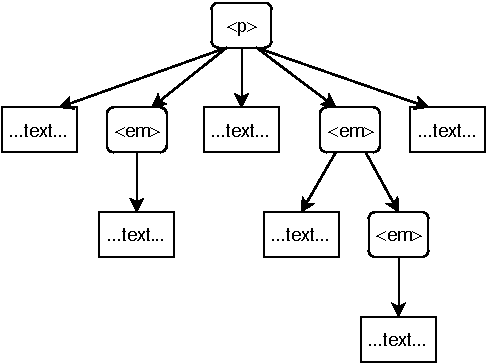
\includegraphics{../../figures/labelling.pdf}
\caption{Labelling a Diagram}
\label{f:exercises-labelling}
\end{figure}

Another way to use diagrams for formative assessment is to give learners
the pieces of the diagram and ask them to arrange them correctly. This
is a visual equivalent of a Parsons Problem, and you can provide as much
or as little of a skeleton to help them with placement as you think
they're ready for. (I have fond memories of trying to place resistors
and capacitors in a circuit diagram in order to get the right voltage at
a certain point, and have often seen teachers give learners a fixed set
of Scratch blocks and ask them to create a particular drawing using only
those blocks.)

\emph{Matching problems} can be thought of as a special case of labelling in
which the ``diagram'' is a column of text and the labels are taken from
the other column. \emph{One-to-one matching} gives the learner two lists of
equal length and asks her to pair corresponding items, e.g., ``match each
piece of code with the output it produces''.

\begin{aside}{Matching}

Match each regular expression operator with what it does.

\begin{longtable}[]{@{}ll@{}}
\texttt{?} & start of line\tabularnewline
\texttt{*} & zero or one occurrences\tabularnewline
\texttt{+} & end of line\tabularnewline
\texttt{\$} & one or more occurrences\tabularnewline
\texttt{\^{}} & zero or more occurrences\tabularnewline
\end{longtable}

\end{aside}

\emph{Many-to-many matching} is similar, but the lists aren't the same
length, so some items may be matched to several others, while others may
not be matched at all. Both kinds require learners to use higher-order
thinking skills, but many-to-many are more difficult because learners
can't do easy matches first to reduce their search space (i.e., there is
a higher cognitive load.)

Matching problems can be implemented by having learners submit lists of
matching pairs as text (such as ``A3, B1, C2''), but that's clumsy and
error-prone. Having them recognize a set of correct pairs in an MCQ is
even worse, as it's painfully easy to misread.

\emph{Ranking} is a special case of matching that is (slightly) more amenable
to answering via lists, since our minds are pretty good at detecting
errors or anomalies in sequences. Give the learner several items and ask
them to order them from fastest to slowest, most robust to most brittle,
and so on. The former tends toward recall (e.g., recognizing the names
of various sorting algorithms and knowing their properties), while the
latter tends more toward reasoning and judgment.

\emph{Summarization} also requires learners to use higher-order thinking, and
gives them a chance to practice a skill that is very useful when
reporting bugs rather than fixing them. For example, learners can be
asked, ``Which sentence best describes how the output of f changes as x
varies from 0 to 10?'' and then given several options as a multiple
choice question.

You can also ask for very short free-form answers to questions in
constrained domains, e.g., ``What is the key feature of a stable sorting
algorithm?'' We still can't fully automate checks for these without a
frustrating number of false positives (accepting wrong answers) and
false negatives (rejecting correct ones), but they lend themselves well
to peer grading (Section~\ref{s:individual-peer}).

\section{Automatic Grading}\label{s:exercises-grading}

Automatic program grading tools have been around longer than I've been
alive: the earliest published mention dates from 1960
\cite{Holl1960}, and the surveys published in
\cite{Douc2005,Ihan2010} mention many specific tools by name.
Building such tools is a lot more complex than it might first seem. How
are assignments represented? How are submissions tracked and reported?
Can learners co-operate? How can submissions be executed safely?
\cite{Edwa2014a} is an entire paper devoted to an adaptive scheme for
detecting and managing infinite loops and other non-terminating code
submissions, and that's just one of the many issues that comes up.

As elsewhere, it's important to distinguish learner satisfaction from
learning outcomes. \cite{Magu2018} switched informal programming labs
to a weekly machine-evaluated test for a second-year CS course using an
auto-grading tool originally developed for programming competitions.
Learners didn't like the automated system, but the overall failure rate
for the course was halved, and the number of learners gaining first
class honors tripled. In contrast, \cite{Rubi2014} also began to use
an auto-grader designed for competitions, but saw no significant
decrease in their learners' dropout rates; once again, learners made
some negative comments about the tool, which the authors attribute to
its feedback messages rather than to dislike of auto-grading.

\cite{Srid2016} took a different approach. They used
\gref{g:fuzz-testing}{fuzz testing} (i.e., randomly-generated
test cases) to check whether learner code does the same thing as a
reference implementation supplied by the teacher. In the first project
of a 1400-learner introductory course, fuzz testing caught errors that
were missed by a suite of hand-written test cases for more than 48\% of
learners, which clearly demonstrates its value.

\cite{Basu2015} gave learners a suite of solution test cases, but
learners had to unlock each one by answering questions about its
expected behavior before they were allowed to apply it to their proposed
solution. For example, suppose learners are writing a function to find
the largest adjacent pair of numbers in a list; before being allowed to
use the tests associated with this question, they have to choose the
right answer to, ``What does \texttt{largestPair(4,\ 3,\ -1,\ 5,\ 3,\ 3)} produce?''
(The correct answer is \texttt{(5,\ 3)}.) In a 1300-person university course,
the vast majority of learners chose to validate their understanding of
test cases this way before attempting to solve problems, and then asked
fewer questions and expressed less confusion about assignments.

It's tempting to use off-the-shelf style checking tools to grade
learners' code. However, \cite{Nutb2016} initially found no
correlation between human-provided marks and style-checker rule
violations. Sometimes this was because learners violated one rule many
times (thereby losing more points than they should have), and other
times it was because they submitted the assignment starter code with few
alterations and got more points than they should have.

\cite{Buff2015} presents a well-informed reflection on
the whole idea of providing automated feedback. Their starting point
is that, ``Automated grading systems help learners identify bugs in
their code, {[}but{]} may inadvertently discourage learners from thinking
critically and testing thoroughly and instead encourage dependence on
the teacher's tests.'' One of the key issues they identified is that a
learner may thoroughly test their code, but the feature may still not
be implemented according to the teacher's specifications. In this
case, the ``failure'' is not caused by a lack of testing, but by a
misunderstanding of the requirements, and it is unlikely that more
testing will expose the problem. If the auto-grading system doesn't
provide insightful, actionable feedback, this experience will only
frustrate the learner.

In order to provide that feedback, \cite{Buff2015}'s system
identifies which method or methods of the learner's code are executed by
failing tests, so that the system can associate failed tests with
particular features within the learner's submission. The system decides
whether specific hints have been ``earned'' by seeing whether the learner
has tested the associated feature enough, so learners cannot rely on
hints instead of doing tests.

\cite{Keun2016a,Keun2016b} classified the messages produced by 69
auto-grading tools. They found that these often do not give feedback on
how to fix problems and take the next step. They also found that most
teachers cannot easily adapt most of the tools to their needs; like many
workflow tools, they tend to enforce their creators' unrecognized
assumptions about how institutions work. Their work is ongoing, and
their detailed classification scheme is a useful shopping list when
looking at tools of this kind.

\cite{Srid2016} discussed strategies for sharing feedback with
learners when automatically testing their code. The first is to provide
the expected output for the tests---but then learners hard-code output for
those inputs (because anything that can be gamed, will be). An
alternative is to report the pass/fail results for the learners' code,
but only supply the actual inputs and outputs of the tests after the
submission date. This can be frustrating, because it tells learners they
are wrong, but not why.

A third option is to use a technique called \gref{g:hashing}{hashing} to
generate a value that depends on the output, but doesn't reveal it. If
the user produces exactly the same output, its hash will be the same
as the hash of the correct output, which will unlock the solution, but
it is impossible to work backward from the hash to figure out what the
output is supposed to be. Hashing is used to create digital signatures
for documents, and requires a bit more work and explanation to set up,
but strikes a good balance between revealing answers prematurely and
not revealing them when it would help.

\section{Higher-Level Thinking}\label{s:exercises-higher}

Many other kinds of programming exercises are hard for teachers to
assess in a class with more than few dozen learners, and equally hard
for automated platforms to assess at all. Larger programming projects,
or projects in which learners set their own goals, are (hopefully) what
classes are building toward. Free-form discussion or twitch coding
(Section~\ref{s:performance-live}) is also valuable, but also doesn't
scale.

\emph{Code review}, on the other hand, is hard to grade automatically in the
general case, but can be tackled if learners are given a rubric (e.g., a
list of faults to look for) and asked to match particular comments
against particular lines of code. For example, the learner can be told
that there are two indentation errors and one bad variable name, and
asked to point them out; if she is more advanced, she could be given
half a dozen kinds of remarks she could make about the code without
guidance as to how many of each she should find.

\cite{Steg2016b} is a good starting point for a code style rubric,
while \cite{Luxt2009} looks at peer review in programming classes
more generally. If you are going to have students do reviews, use
calibrated peer review (Section~\ref{s:individual-peer}) so that they
have models of what good feedback should look like.

\begin{aside}{Code Review}

Using the rubric provided, mark each line of the code below.

\begin{minted}{text}
01)  def addem(f):
02)      x1 = open(f).readlines()
03)      x2 = [x for x in x1 if x.strip()]
04)      changes = 0
05)      for v in x2:
06)          print('total', total)
07)          tot = tot + int(v)
08)      print('total')
\end{minted}

\begin{enumerate}
\item
  poor variable name
\item
  unused variable
\item
  use of undefined variable
\item
  missing return value
\end{enumerate}

\end{aside}

\section{Exercises}\label{s:exercises-exercises}

\subsection*{Code and Run (pairs/10)}

Create a short C\&R exercise; trade with a partner, and see how long it
takes each of you to understand and do the other's exercise. Were there
any ambiguities or misunderstandings in the exercise description?

\subsection*{Inverting Code and Run (small groups/15)}

Form groups of 4--6 people. Have each member of the group create an
inverted C\&R exercise that requires people to figure out what input
produces a particular output. Pick two at random, and see how many
different inputs the group can find that satisfy the requirements.

\subsection*{Tracing Values (pairs/10)}

Write a short program (10--15 lines); trade with a partner, and trace how
the variables in the program change value over time. What differences
are there in how you and your partner wrote down your traces?

\subsection*{Refactoring (small groups/15)}

Form groups of 3--4 people. Have each person select a short piece of code
(10--30 lines long) that they have written that isn't as tidy as it could
be. Choose one at random, and have everyone in the group tidy it up
independently. How do your cleaned-up versions differ? How well or how
poorly would you be able to accommodate all of these variations if
marking automatically or in a large class?

\subsection*{Labelling a Diagram (pairs/10)}

Draw a diagram showing something that you have explained recently: how
browsers fetch data from servers, the relationship between objects and
classes, or how data frames are indexed in R. Put the labels on the
side, and ask your partner to place them.

\subsection*{Pencil-and-Paper Puzzles (whole class/15)}

\cite{Butl2017} describes a set of pencil-and-paper puzzles that can
be turned into introductory programming assignments, and found that
these assignments are enjoyed by students and encourage meta-cognition.
Think of a simple pencil-and-paper puzzle or game you played as a child,
and describe how you would turn it into a programming exercise.

\subsection*{Counting Failures (pairs/15)}

Any useful estimate of how much time an exercise needs must take into
account how frequent failures are and how much time is lost to them. For
example, editing text files seems like a simple task, but what about
finding those files? Most GUI editors save things to the user's desktop
or home directory; if the files used in a course are stored somewhere
else, a substantial fraction won't be able to navigate to the right
directory without help. (If this seems like a small problem to you,
please revisit the discussion of expert blind spot in
Chapter~\ref{s:memory}.)

Working with a partner, make a list of ``simple'' things you have seen go
wrong in exercises you have used or taken. How often do they come up?
How long do they take learners to fix on their own, or with help? How
much time do you currently budget in class to deal with them?

\chapter{Building Community}\label{s:community}

\begin{objectives}

\item
  Explain what situated learning is and identify its key elements.

\item
  Explain how to decide whether to try to create a new community or
  join an existing effort.

\item
  Outline a three-step plan for recruiting, retaining, and retiring
  volunteers and other organization participants.

\item
  Explain the difference between a service board and a governance
  board, and judge which kind an organization has.

\end{objectives}

Many well-intentioned people want the world to be a better place, but
don't actually want anything important to change. A lot of grassroots
efforts to teach programming fall into this category: they want to teach
children and adults how to program so that they can get good jobs,
rather than empower them to change the system that has shut them (and
people like them) out of those jobs in the past.

If you are going to build a community, the first and most important
thing you have to decide is what \emph{you} want: to help people
succeed in the world we have, or to give them a way to make a better
one.  Either way, you have to accept that one person can only do so
much. Just as we learn best together, we teach best when we are
teaching with other people, and the best way to achieve that is to
build a community.

And as Anu Partanen
\href{https://www.theatlantic.com/national/archive/2011/12/what-americans-keep-ignoring-about-finlands-school-success/250564/}{pointed
  out}, sometimes you need to fix several things in order to fix one.
Finland's teachers aren't successful in isolation: they are able to
achieve outstanding results because their country's citizens truly
value equality of opportunity.  People (and countries) that try to
adopt their teaching methods without ensuring that children (and
parents) are well nourished, safe, and treated fairly by the courts
will have a more difficult time.  This doesn't mean you have to fix
all of society's ills in order to teach programming, but it
\emph{does} mean that you have to understand and be involved in what
happens to your learners outside of your class if you want that class
to work.

A framework in which to think about educational communities is
\glossref{g:situated-learning}{situated learning}, which focuses on
how \glossref{g:legitimate-peripheral-participation}{legitimate
  peripheral participation} leads to people becoming members of a
\glossref{g:community-of-practice}{community of practice}
\cite{Weng2015}.  Unpacking those terms, a community of practice is a
group of people bound together by interest in some activity, such as
knitting or particle physics. Legitimate peripheral participation
means doing simple, low-risk tasks that community nevertheless
recognizes as valid contributions: making your first scarf, stuffing
envelopes during an election campaign, or proof-reading documentation
for open source software.

Situated learning focuses on the transition from being a newcomer to
being accepted as a peer by those who are already community members.
This typically means starting with simplified tasks and tools, then
doing similar tasks with more complex tools, and finally tackling the
exercises of advanced practitioners. For example, children learning
music may start by playing nursery rhymes on a recorder or ukulele,
then play other simple songs on a trumpet or saxophone in a band, and
finally start exploring their own musical tastes. Healthy communities
of practice understand and support these progressions, and recognize
that each step is meant to give people a ramp rather than a cliff.
Some of the ways they do this include:

\begin{description}

\item[Problem solving:] ``I'm stuck---Can we work on this design and
  brainstorm some ideas?''

\item[Requests for information:] ``Where can I find the code to
  connect to the server?''

\item[Seeking experience:] ``Has anyone dealt with a customer in this
  situation?''

\item[Reusing assets:] ``I have a proposal for an event website that I
  wrote for a client last year you can use as a starting point.''

\item[Coordination and synergy:] ``Can we combine our purchases of web
  hosting to get a discount?''

\item[Building an argument:] ``How do people in other companies do
  this?  Armed with this information it will be easier to convince my
  CEO to make some changes.''

\item[Growing confidence:] ``Before I do it, I'll run it through my
  community first to see what they think.''

\item[Discussing developments:] ``What do you think of the new work
  tracking system?  Does it really help?''

\item[Documenting projects:] ``We have faced this problem five times
  now. Let us write it down once and for all.''

\item[Visits:] ``Can we come and see your after-school program? We
  need to establish one in our city.''

\item[Mapping knowledge and identifying gaps:] ``Who knows what, and
  what are we missing? What other groups should we connect with?''

\end{description}

Whatever the domain, situated learning emphasizes that learning is a
social activity.  In order to be effective and sustainable, teaching
therefore needs to be rooted in a community; if one doesn't exist, you
need to build one.  There are at least
\href{https://www.feverbee.com/types-of-community-and-activity-within-the-community/}{four
  types}:

\begin{description}

\item[Community of action:] people focused on a shared goal, such as
  getting someone elected.

\item[Community of concern:] members are brought together by a shared
  exercise, such as dealing with depression.

\item[Community of interest:] focused on a shared love of something
  like backgammon or knitting.

\item[Community of place:] of people who happen to live or work side
  by side.

\end{description}

Most real communities are mixes of these, such as people in Toronto
who like teaching tech; what matters is that you pick something and
stick with it.

\section{Learn, Then Do}\label{s:community-learn-then-do}

The first step in building a community is to decide if you really need
to, or whether you would be more effective joining an existing
organization. Thousands of groups are already teaching people tech
skills, from the \href{http://www.4-h-canada.ca/}{4-H Club} and
\href{https://www.frontiercollege.ca/}{literacy programs} to
get-into-coding non-profits like
\href{http://www.blackgirlscode.com/}{Black Girls Code} and
\href{http://bridgeschool.io/}{Bridge}. Joining an existing group will
give you a head start on teaching, an immediate set of colleagues, and
a chance to learn more about how to run things; hopefully, learning
those skills will be more important than being able to say that you're
the founder or leader of something new.

Whether you join an existing group or set up one of your own, you owe
it to yourself and everyone who's going to work with you to find out
what's been done before. People have been writing about grassroots
organizing for decades; \cite{Alin1989} is probably the best-known
work on the subject, while \cite{Brow2007,Midw2010} are practical
manuals rooted in decades of practice. If you want to read more
deeply, \cite{Adam1975} is a history of the Highlander Folk School,
whose approach has been emulated by many successful groups, while
\cite{Spal2014} is a guide to teaching adults written by someone with
deep personal roots in organizing, and
\href{https://www.nonprofitready.org/}{NonprofitReady.org} offers free
professional development training.

\section{Three Steps}\label{s:community-three-steps}

Everyone who gets involved with your organization, including you, goes
through three phases: recruitment, retention, and retirement (from the
organization). You don't need to worry about this cycle when you're just
getting started, but it \emph{is} worth thinking about as soon as you
have more than a couple of non-founders involved.

The first step is recruiting volunteers. Your marketing should help
you with this by making your organization findable, and by making its
mission and its value to volunteers clear to people who might want to
get involved. Share stories that exemplify the kind of help you want
as well as stories about the people you're helping, and make it clear
that there are many ways to get involved. (We discuss this in more
detail in the next section.)

Your best source of new recruits is your own classes: ``see one, do one,
teach one'' has worked well for volunteer organizations for as long as
there have \emph{been} volunteer organizations. Make sure that every
class or other encounter ends with two sentences explaining how people
can help, and that help is welcome. People who come to you this way will
know what you do, and will have recent experience of being on the
receiving end of what you offer that they can draw on, which helps your
organization avoid collective
\glossref{g:expert-blind-spot}{expert blind spot}.

\begin{callout}{Start Small}

  As \href{https://en.wikipedia.org/wiki/Ben\_Franklin\_effect}{Ben
    Franklin} observed, a person who has performed a favor for someone
  is more likely to do another favor for that person than they would
  be if they had received a favor from that person. Asking people to
  do something small for you is therefore a good step toward getting
  them to do something larger. One natural way to do this when
  teaching is to ask people to submit fixes for your lesson materials
  for typos or unclear wording, or to suggest new exercises or
  examples. If your materials are written in a maintainable way
  (\secref{s:process-maintainability}), this gives them a chance to
  practice some useful skills, and gives you an opportunity to start a
  conversation that might lead to a new recruit.

\end{callout}

Recruiting doesn't end when someone first shows up: if you don't
follow through, people will come out once or twice, then decide that
what you're doing isn't for them and disappear. One thing you can do
to get newcomers over this initial hump is to have them take part in
group activities before they do anything on their own, both so that
they get a sense of how your organization does things, and so that
they build social ties that will keep them involved.

Another thing you can do is give newcomers a mentor, and make sure the
mentors actually do some proactive mentoring. The most important
things a mentor can do are make introductions and explain the
unwritten rules, so make it clear to mentors that these are their
primary responsibilities, and they are to report back to you every few
weeks to tell you what they've done.

The second part of the volunteer lifecycle is retention, which is a
large enough topic to deserve a long discussion in
\secref{s:community-retention}.  The third and final part is
retirement. Sooner or later, everyone moves on (including you). When
this happens:

\begin{description}

\item[Ask people to be explicit about their departure] so that
  everyone knows they've actually left.

\item[Make sure they don't feel embarrassed or ashamed about leaving.]

\item[Give them an opportunity to pass on their knowledge.] For
  example, you can ask them to mentor someone for a few weeks as their
  last contribution, or to be interviewed by someone who's staying
  with the organization to collect any stories that are worth
  re-telling.

\item[Make sure they hand over the keys.] It's awkward to discover six
  months after someone has left that they're the only person who knows
  how to book a playing field for the annual softball game.

\item[Follow up 2--3 months after they leave] to see if they have any
  further thoughts about what worked and what didn't while they were
  with you, or any advice to offer that they either didn't think to
  give or were uncomfortable giving on their way out the door.

\item[Thank them,] both when they leave and the next time your group
  gets together.

\end{description}

\section{Retention}\label{s:community-retention}

Saul Alinsky once said, ``If your people aren't having a ball doing
it, there is something very wrong.'' \cite{Alin1989} Community members
shouldn't expect to enjoy every moment of their work with your
organization, but if they don't enjoy any of it, they won't stay.

Enjoyment doesn't necessarily mean having an annual party: people may
enjoy cooking, coaching, or just working quietly beside others. There
are several things every organization should do to ensure that people
are getting something they value out of their work:

\begin{description}

\item[Ask people what they want rather than guessing.] Just as you are
  not your learners (\secref{s:process-personas}), you are probably
  different from other members of your organization. Ask people what
  they want to do, what they're comfortable doing (which may not be
  the same thing), what constraints there are on their time, and so
  on.  They might start by saying, ``I don't know---anything!'' but
  even a short conversation will probably uncover the fact that they
  like interacting with people but would rather not be managing the
  group's finances, or vice versa.

\item[Provide many ways to contribute.] The more ways there are for
  people to help, the more people will be able to help. Someone who
  doesn't like standing in front of an audience may be able to
  maintain your organization's website or handle its accounts; someone
  who doesn't know how to do anything else may be able to proof-read
  lessons, and so on. The more kinds of tasks you do yourself, the
  fewer opportunities there are for others to get involved.

\item[Recognize contributions.] Everyone likes to be appreciated, so
  communities should acknowledge their members' contributions both
  publicly and privately by mentioning them in presentations, putting
  them on the website, and so on.

\item[Make space.] Micromanaging or trying to control everything
  centrally means people won't feel they have the autonomy to act,
  which will probably cause them to drift away. In particular, if
  you're too engaged or too quick on the reply button, people have
  less opportunity to grow as members and to create horizontal
  collaborations.  As a result, the community will continue to be
  focused around one or two individuals, rather than a
  highly-connected network in which others feel comfortable
  participating.

\end{description}

Another way to make participation rewarding is to provide training.
Organizations require committees, meetings, budgets, grant proposals,
and dispute resolution; most people are never taught how to do any of
this, any more than they are taught how to teach, but training people to
do these things helps your organization run more smoothly, and the
opportunity to gain transferable skills is a powerful reason for people
to get and stay involved. If you are going to do this, don't try to
provide the training yourself (unless it's what you specialize in). Many
civic and community groups have programs of this kind, and you can
probably make a deal with one of them.

Other groups may be useful in other ways as well, and you may be useful
to them---if not immediately, then tomorrow or next year. You should
therefore set aside an hour or two every month to find allies and
maintain your relationships with them. One way to do this is to ask them
for advice: how do they think you ought to raise awareness of what
you're doing? Where have they found space to run classes? What needs do
they think aren't being met, and would you be able to meet them (either
on your own, or in partnership with them)? Any group that has been
around for a few years will have useful advice; they will also be
flattered to be asked, and will know who you are the next time you call.

\begin{callout}{Government Matters}

  It's fashionable in tech circles to disparage government
  institutions as slow-moving dinosaurs, but in my experience they are
  no worse than companies of similar size.  Your local school board,
  library, and your city councillor's office may be able to offer
  space, funding, publicity, connections with other groups that you
  may not have met yet, help with red tape, and a host of other useful
  things.

\end{callout}

\begin{callout}{Soup, Then Hymns}

  Manifestos are fun to write, but most people join a volunteer
  community to help and be helped rather than to argue over the
  wording of a grand vision statement. (Most people who prefer the
  latter are \emph{only} interested in arguing{\ldots}) To be
  effective you should therefore focus on things that are immediately
  useful, e.g., on what people can create that will be used by other
  community members right away. Once your organization shows that it
  can actually achieve small things, people will be more confident
  that it's worth investing in bigger ones.  That's the time to worry
  about manifestos, since that's the point at which it's important to
  define values that will guide your growth and operations.

\end{callout}

One important special case of making things rewarding is to pay
people.  Volunteers can do a lot, but eventually tasks like system
administration and accounting need full-time paid staff.  When this
time comes, you should either pay people nothing or pay them a proper
wage, but not do anything in between.  If you pay them nothing, their
actual reward for their work is the satisfaction of doing good.  If
you pay them a token amount, you take that away without giving them
the satisfaction of earning a living.

\subsection*{Impostor Syndrome}

Impostor syndrome thrives in communities with arbitrary, unnecessary
standards, where harsh criticism is the norm, and where secrecy
surrounds the actual process of getting work done, so the Ada
Initiative has
\href{https://www.usenix.org/blog/impostor-syndrome-proof-yourself-and-your-community}{guidelines}
for communities to go with those given in
\secref{s:motivation-demotivation}for individuals:

\begin{description}

\item[Simply encourage people.]

\item[Discourage hostility and bickering.] Public, hostile, personal
  arguments are a natural breeding ground for impostor syndrome.

\item[Eliminate hidden barriers to participation.] Be explicit about
  welcoming new students and colleagues, and thoroughly document how
  someone can participate in projects and events in your research
  group and at your institution.

\item[As a leader, show your own uncertainties and demonstrate your
  own learning process.] When people see leaders whom they respect
  struggling or admitting they didn't already know everything when
  they started, having realistic opinions of their own work becomes
  easier.

\item[Reward and encourage people in your team and department for
  mentoring newcomers.] Officially enshrine mentoring as an important
  criterion in your career advancement process.

\item[Don't make it personal when someone's work isn't up to snuff.]
  When enforcing necessary quality standards, don't make the issue
  about the person. They aren't wrong or stupid or a waste of space;
  they've simply done one piece of work that didn't meet your
  expectations.

\end{description}

\section{Governance}\label{s:community-governance}

As \cite{Free1972} pointed out, every organization has a power
structure: the only question is whether it's formal and accountable,
or informal and unaccountable. Make yours one of the first kind: write
and publish the rules governing everything from who's allowed to use
the name and logo to who gets to decide whether people are allowed to
charge money to teach with whatever materials your group has worked
up.

Organizations can govern themselves in many different ways, and a full
discussion of the options is outside the scope of this book.
For-profit corporations and incorporated non-profits the two most
popular models; the mechanics vary from jurisdiction to jurisdiction,
so you should seek advice locally before doing anything.  (This is one
of the times when having ties with local government or other
like-minded organizations pays off.)

The model I prefer is that of a commons, which is ``something managed
jointly by a community according to rules they themselves have evolved
and adopted''.  As \cite{Boll2014} emphasizes, all three parts of that
definition are essential: a commons isn't just a shared pasture, but
also includes the community that shares it and the rules they use to
do so.

Most resources, throughout most of human history, have been commons:
it is only in the last few hundred years that impersonal markets have
pushed them to the margins. In order to do so, free-market advocates
have had to convince us we're something we're not (dispassionate
calculators of individual advantage) and erase or devalue local
knowledge and custom with tragic consequences for us individually and
collectively.

Since society has difficulty recognizing commons organizations, and
since most of the people you will want to recruit don't have experience
with them, you will probably wind up having some sort of board, a
director, and other staff. Broadly speaking, your organization can have
either a \emph{service board}, whose members also take on other roles in
the organization, or a \emph{governance board} whose primary
responsibility is to hire, monitor, and if need be fire the director.
Board members can be elected by the community or appointed; in either
case, it's important to prioritize competence over passion (the latter
being more important for the rank and file), and to try to recruit for
particular skills such as accounting, marketing, and so on.

Don't worry about drafting a constitution when you first get started: it
will only result in endless wrangling about what we're going to do
rather than formalization of what you're already doing. When the time
does come to formalize your rules, though, make your organization a
democracy: sooner or later (usually sooner), every appointed board turns
into a mutual agreement society and loses sight of what the community
it's meant to serve actually needs. Giving the community power is messy,
but is the only way invented so far to ensure that an organization
continues to meet people's actual needs.

\section{Final Thoughts}\label{s:community-final}

As \cite{Pign2016} discusses, burnout is a chronic risk in any
community activity. If you don't take care of yourself, you won't be
able to take care of your community.

Every organization eventually needs fresh ideas and fresh leadership.
When that time comes, train your successors and then move on. They will
undoubtedly do things you wouldn't have, but the same is true of every
generation. Few things in life are as satisfying as watching something
you helped build take on a life of its own. Celebrate that---you won't
have any trouble finding something else to keep you busy.

\section{Exercises}\label{s:community-exercises}

Several of these exercises are taken from \cite{Brow2007}, which is
an exceptionally useful book on building community organizations.

\exercise{What Kind of Community?}{individual}{15}

Re-read the discussion in the introduction of types of communities and
decide which type or types your group is, or aspires to be.

\exercise{People You May Meet}{small groups}{30}

As an organizer, part of your job is sometimes to help people find a way
to contribute despite themselves. In small groups, pick three of the
people below and discuss how you would help them become a better
contributor to your organization.

\begin{description}

\item[Anna] knows more about every subject than everyone else put
  together---at least, she thinks she does. No matter what you say,
  she'll correct you; no matter what you know, she knows better.

\item[Catherine] has so little confidence in her own ability that she
  won't make any decision, no matter how small, until she has checked
  with someone else.

\item[Frank] believes that knowledge is power, and enjoys knowing
  things that other people don't. He can make things work, but when
  asked how he did it, he'll grin and say, ``Oh, I'm sure you can
  figure it out.''

\item[Hediyeh] is quiet. She never speaks up in meetings, even when
  she knows that what other people are saying is wrong. She might
  contribute to the mailing list, but she's very sensitive to
  criticism, and will always back down rather than defending her point
  of view.

\item[Kenny] has discovered that most people would rather shoulder his
  share of the work than complain about him, and he takes advantage of
  it at every turn. The frustrating thing is that he's so damn
  \emph{plausible} when someone finally does confront him. ``There
  have been mistakes on all sides,'' he says, or, ``Well, I think
  you're nit-picking.''

\item[Melissa] means well, but somehow something always comes up, and
  her tasks are never finished until the last possible moment. Of
  course, that means that everyone who is depending on her can't do
  their work until \emph{after} the last possible moment{\ldots}

\item[Raj] is rude. ``It's just the way I talk,'' he says, ``If you
  can't hack it, maybe you should find another team.'' His favorite
  phrase is, ``That's stupid,'' and he uses obscenity in every second
  sentence.

\end{description}

\exercise{Values}{small groups}{45}

Answer the following questions on your own, and then compare your
answers to those given by other members of your group.

\begin{enumerate}

\item
  What are the values your organization expresses?

\item
  Are these the values you want the organization to express?

\item
  If not, what values would you like it to express?

\item
  What are the specific behaviors that demonstrate those values?

\item
  What are some key behaviors that would demonstrate the values you
  would like for your group?

\item
  What are the behaviors that would demonstrate the opposite of those
  values?

\item
  What are some key behaviors that would demonstrate the opposite of the
  values you want to have?

\end{enumerate}

\exercise{Meeting Procedures}{small groups}{30}

Answer the following questions on your own, and then compare your
answers to those given by other members of your group.

\begin{enumerate}

\item
  How are your meetings run?

\item
  Is this how you want your meetings to be run?

\item
  Are the rules for running meetings explicit or just assumed?

\item
  Are these the rules you want?

\item
  Who is eligible to vote/make decisions?

\item
  Is this who you want to be vested with decision-making authority?

\item
  Do you use majority rule, make decisions by consensus, or use some
  other method?

\item
  Is this the way you want to make decisions?

\item
  How do people in a meeting know when a decision has been made?

\item
  How do people who weren't at a meeting know what decisions were made?

\item
  Is this working for your group?

\end{enumerate}

\exercise{Size}{small groups}{20}

Answer the following questions on your own, and then compare your
answers to those given by other members of your group.

\begin{enumerate}

\item
  How big is your group?

\item
  Is this the size you want for your organization?

\item
  If not, what size would you like it to be?

\item
  Do you have any limits on the size of membership?

\item
  Would you benefit from setting such a limit?

\end{enumerate}

\exercise{Staffing}{small groups}{30}

Answer the following questions on your own, and then compare your
answers to those given by other members of your group.

\begin{enumerate}

\item
  Do you have paid staff in your organization?

\item
  Or is it all-volunteer?

\item
  Should you have paid staff?

\item
  Do you want/need more or less staff?

\item
  What do you call the staff (e.g., organizer, director, coordinator,
  etc.)?

\item
  What do the staff members do?

\item
  Are these the primary roles and functions that you want the staff to
  be filling?

\item
  Who supervises your staff?

\item
  Is this the supervision process and responsibility chain that you want
  for your group?

\item
  What is your staff paid?

\item
  Is this the right salary to get the needed work done and to fit within
  your resource constraints?

\item
  What benefits does your group provide to its staff (health, dental,
  pension, short and long-term disability, vacation, comp time, etc.)?

\item
  Are these the benefits that you want to give?

\end{enumerate}

\exercise{Money}{small groups}{30}

Answer the following questions on your own, and then compare your
answers to those given by other members of your group.

\begin{enumerate}

\item
  Who pays for what?

\item
  Is this who you want to be paying?

\item
  Where do you get your money?

\item
  Is this how you want to get your money?

\item
  If not, do you have any plans to get it another way?

\item
  If so, what are they?

\item
  Who is following up to make sure that happens?

\item
  How much money do you have?

\item
  How much do you need?

\item
  What do you spend most of your money on?

\item
  Is this how you want to spend your money?

\end{enumerate}

\exercise{Becoming a Member}{small groups}{45}

Answer the following questions on your own, and then compare your
answers to those given by other members of your group.

\begin{enumerate}

\item
  How does someone join?

\item
  Does this process work for your organization?

\item
  What are the membership criteria?

\item
  Are these the membership criteria you want?

\item
  Are people required to agree to any rules of behavior upon joining?

\item
  Are these the rules for behavior you want?

\item
  Are there membership dues?

\end{enumerate}

\exercise{Borrowing Ideas}{whole class}{15}

Many of our ideas about how to build a community have been shaped by
our experience of working in open source software development.
\cite{Foge2005} (which is \href{http://producingoss.com/}{available
  online}) is a good guide to what has and hasn't worked for those
communities, and the \href{https://opensource.guide/}{Open Source
  Guides site} has a wealth of useful information as well.  Choose one
section of the latter, such as ``Finding Users for Your Project'' or
``Leadership and Governance'', read it through, and give a two-minute
presentation to the group of one idea from it that you found useful or
that you strongly disagreed with.

\exercise{Who Are You?}{small groups}{20}

The National Oceanic and Atmospheric Administration (NOAA) has
published a short, amusing, and above all useful guide to
\href{https://coast.noaa.gov/ddb/story_html5.html}{dealing with
  disruptive behaviors}. It categorizes those behaviors under labels
like ``talkative'', ``indecisive'', and ``shy'', and outlines
strategies for handling each.  In groups of 3--6, read the guide and
decide which of these descriptions best fits you.  Do you think the
strategies described for handling people like you are effective?  Are
other strategies equally or more effective?

\chaplbl{Outreach}{s:outreach}

It's fashionable in tech circles
to disparage universities and government institutions as slow-moving dinosaurs,
but in my experience they are no worse than companies of similar size.
Your local school board, library, and your city councillor's office
may be able to offer space, funding, publicity,
connections with other groups that you may not have met yet,
and a host of other useful things;
getting to know them can help you solve or avoid problems in the short term
and pay dividends down the road.

\seclbl{Marketing}{s:outreach-marketing}

People with academic or technical backgrounds often think that
\gref{g:marketing}{marketing} is about spin and misdirection.
In reality,
it's about seeing things from other people's perspective,
understanding their wants and needs,
and explaining how you can help them---in short,
how to teach them.
This chapter will look at how to use ideas from the previous chapters
to get people to understand and support what you're doing.

The first step is to figure out what you are offering to whom,
i.e.,
what actually brings in the volunteers,
funding,
and other support you need to keep going.
The answer is often counter-intuitive.
For example,
most scientists think their papers are their product,
but it's actually their grant proposals,
because those are what brings in grant money~\cite{Kuch2011}.
Their papers are the advertising that persuades people to fund those proposals,
just as albums are now what persuades people to buy musicians' concert tickets and t-shirts.

Suppose that your group offers weekend programming workshops
to people who are re-entering the workforce after being away for several years.
If workshop participants can pay enough to cover your costs,
then they are your customers and the workshops are the product.
If,
on the other hand,
the workshops are free or the learners are only paying a token amount to cut the no-show rate,
then your actual product may be some mix of:

\begin{itemize}

\item
  your grant proposals;

\item
  the alumni of your workshops
  that the companies sponsoring you would like to hire;

\item
  the half-page summary of your workshops in the mayor's annual report to city council
  that shows how she's supporting the local tech sector;
  or

\item
  the personal satisfaction that volunteers get from teaching.

\end{itemize}

As with lesson design (\chapref{s:process}),
the first steps in marketing are
to create personas\index{learner persona}
of people who might be interested in what you're doing
and to figure out which of their needs you can meet.
One way to summarize the latter is to write \grefdex{g:elevator-pitch}{elevator pitches}{elevator pitch}
aimed at different personas.
A widely-used template for these is:

\newpage
\begin{longtable}{ll}
  For 		& \emph{target audience} \\
  who 		& \emph{dissatisfaction with what's currently available} \\
  our 		& \emph{category} \\
  provide 	& \emph{key benefit}. \\
  Unlike 	& \emph{alternatives} \\
  our program 	& \emph{key distinguishing feature.}
\end{longtable}

\noindent
Continuing the weekend workshop example,
we could use this pitch for participants:

\begin{quote}

  For \emph{people re-entering the workforce after being away for several years}
  who \emph{still have family responsibilities},
  our \emph{introductory programming workshops}
  provide \emph{weekend classes with on-site childcare}.
  Unlike \emph{online classes},
  our program \emph{gives people a chance to meet others at the same stage of life}.

\end{quote}

\noindent
and this one for decision makers at companies that might sponsor the workshops:

\begin{quote}

  For \emph{companies that want to recruit entry-level software developers}
  that \emph{struggle to find mature candidates from diverse backgrounds}
  our \emph{introductory programming workshops}
  provide \emph{potential recruits}.
  Unlike \emph{college recruiting fairs},
  our program \emph{connects companies with a wide variety of candidates}.

\end{quote}

If you don't know why different potential stakeholders might be interested in what you're doing,
ask them.
If you do know,
ask them anyway:
answers can change over time,
and you may discover things you previously overlooked.

Once you have these pitches,
they should drive what you put on your web site and in publicity material
to help people figure out as quickly as possible
if you and they have something to talk about.
(You probably \emph{shouldn't} copy them verbatim,
though:
many people in tech have seen this template so often that
their eyes will glaze over if they encounter it again.)

As you are writing these pitches,
remember that there are many reasons to learn how to program
(\secref{s:intro-exercises}).
A sense of accomplishment,
control over their own lives,
and being part of a community may motivate people more than money
(\chapref{s:motivation}).
They might volunteer to teach with you because their friends are doing it;
similarly,
a company may say that they're sponsoring classes for economically disadvantaged high school students
because they want a larger pool of potential employees further down the road,
but the CEO might actually be doing it simply because it's the right thing to do.

\seclbl{Branding and Positioning}{s:outreach-branding}

A \gref{g:brand}{brand} is someone's first reaction to a mention of a product;
if the reaction is ``what's that?'',
you don't have a brand (yet).
Branding is important because
people aren't going to help something they don't know about or don't care about.

Most discussion of branding today focuses on
how to build awareness online.
Mailing lists,
blogs,
and Twitter all give you ways to reach people,
but as the volume of misinformation increases,
people pay less attention to each individual interruption.
This makes \gref{g:positioning}{positioning} ever more important.
Sometimes called ``differentiation'',
it is what sets your offering apart from others---the ``unlike'' section of your elevator pitches.
When you reach out to people who are already familiar with your field,
you should emphasize your positioning,
since it's what will catch their attention.

There are other things you can do to help build your brand.
One is to use props
like a robot that one of your learners made from scraps she found around the house~\cite{Schw2013}
or the website another learner made for his parents' retirement home.
Another is to make a short video---no more than a few minutes long---that showcases
the backgrounds and accomplishments of your learners.
The aim of both is to tell a story:
while people always ask for data,
they believe and remember stories.

\begin{aside}{Foundational Myths}
  One of the most compelling stories a person or group can tell is
  why and how they got started.
  Are you teaching what you wish someone had taught you but didn't?
  Was there one particular person you wanted to help,
  and that opened the floodgates?
  If there isn't a section on your website starting, ``Once upon a time,''
  think about adding one.
\end{aside}

One crucial step is to make your organization findable in online searches.\index{findability!of organizations}
\cite{DiSa2014b} discovered that
the search terms that parents used for out-of-school computing classes
didn't actually find those classes,
and many other groups face similar challenges.
There's a lot of folklore about how to make things findable
(otherwise known as \gref{g:seo}{search engine optimization} or SEO);
given Google's near-monopoly powers and lack of transparency,
most of it boils down to trying to stay one step ahead of
algorithms designed to prevent people from gaming rankings.

Unless you're very well funded,
the best you can do is to search for yourself and your organization on a regular basis
and see what comes up,
then read \hreffoot{https://moz.com/learn/seo/on-page-factors}{these guidelines}
and do what you can to improve your site.
Keep \hreffoot{https://xkcd.com/773/}{this XKCD cartoon} in mind:
people don't want to know about your org chart or get a virtual tour of your site---they want your address,
parking information,
and some idea of what you teach,
when you teach it,
and how it's going to change their lives.

\begin{aside}{Not Everyone Lives Online}
  These examples assume people have access to the internet
  and that groups have money, materials, free time, and/or technical skills.
  Many don't---in fact,
  those serving economically disadvantaged groups almost certainly don't.
  (As Rosario Robinson says, ``Free works for those that can afford free.'')\index{Robinson, Rosario}
  Stories are more important than course outlines in those situations
  because they are easier to retell.
  Similarly,
  if the people you hope to reach are not online as often as you,
  then notice boards in schools,
  local libraries,
  drop-in centers,
  and grocery stores may be the most effective way to reach them.
\end{aside}

\seclbl{The Art of the Cold Call}{s:outreach-cold-call}

Building a web site and hoping that people find it is easy;
calling people up or knocking on their door without any sort of prior introduction
is much harder.
As with standing up and teaching,
though,
it's a craft that can be learned.
Here are ten simple rules for talking people into things:

\begin{description}

\item[1: Don't.]
  If you have to talk someone into something,
  odds are that they don't really want to do it.
  Respect that:
  it's almost always better in the long run to leave some particular thing undone
  than to use guilt or any underhanded psychological tricks that will only engender resentment.

\item[2: Be kind.]
  I don't know if there actually is a book called
  ``Secret Tricks of the Ninja Sales Masters'',
  but if there is,
  it probably tells readers that doing something for a potential customer
  that creates a sense of obligation,
  which in turn increases the odds of a sale.
  That may work, but it only works once and it's a skeezy thing to do.
  On the other hand,
  if you are genuinely kind
  and help other people because it's what good people do,
  you just might inspire them to be good people too.

\item[3: Appeal to the greater good.]
  If you open by talking about what's in it for them,
  you are signalling that they should think of their interaction with you
  as a commercial exchange of value to be bargained over.
  Instead,
  start by explaining how whatever you want them to help with is going to make the world a better place,
  and \emph{mean it}.
  If what you're proposing isn't going to make the world a better place,
  propose something better.

\item[4: Start small.]
  Most people are understandably reluctant to dive into things head-first,
  so give them a chance to test the waters
  and to get to know you and everyone else involved in
  whatever it is you want help with.
  Don't be surprised or disappointed if that's where things end:
  everyone is busy or tired or has projects of their own,
  or maybe just has a different mental model of how collaboration is supposed to work.
  Remember the 90-9-1 rule---90\% of people will watch,
  9\% will speak up,
  and 1\% will actually do things---and set your expectations accordingly.

\item[5: Don't build a project: build a community.]
  I used to belong to a baseball team that never actually played baseball:
  our ``games'' were just an excuse for us to hang out and enjoy each other's company.
  You probably don't want to go quite that far,
  but sharing a cup of tea with someone or celebrating the birth of their first grandchild
  can get you things that no reasonable amount of money can.

\item[6: Establish a point of connection.]
  ``I was speaking to X'' or ``we met at Y'' gives them context,
  which in turn makes them more comfortable.
  This must be specific:
  spammers and cold-callers have trained us all to ignore anything that starts,
  ``I recently came across your website{\ldots}''

\item[7: Be specific about what you are asking for.]
  People need to know this
  so that they can figure out whether the time and skills they have
  are a match for what you need.
  Being realistic up front is also a sign of respect:
  if you tell people you need a hand moving a few boxes
  when you're actually packing up an entire house,
  they're probably not going to help you a second time.

\item[8: Establish your credibility.]
  Mention your backers,
  your size,
  how long your group has been around, or something that you've accomplished in the past
  so that they'll believe you're worth taking seriously.

\item[9: Create a slight sense of urgency.]
  ``We're hoping to launch this in the spring'' is more likely to get a positive response
  than ``We'd eventually like to launch this.''
  However, the word ``slight'' is important:
  if your request is urgent,
  most people will assume you're disorganized or that something has gone wrong
  and may then err on the side of prudence.

\item[10: Take a hint.]
  If the first person you ask for help says no,
  ask someone else.
  If the fifth or the tenth person says no,
  ask yourself if what you're trying to do makes sense and is worth doing.

\end{description}

The email template follows all of these rules.
It has worked pretty well:
we found that about half of emails were answered,
about half of those wanted to talk more,
and about half of those led to workshops,
which means that 10--15\% of targeted emails turned into workshops.
That can still be pretty demoralizing if you're not used to it,
but is much better than the 2--3\% response rate most organizations expect with cold calls.

\begin{quote}

  \noindent
  Hi NAME,

  I hope you don't mind mail out of the blue,
  but I wanted to follow up on our conversation at VENUE
  to see if you would be interested having us run a teacher training workshop---we're
  scheduling the next batch over the next couple of weeks.

  This one-day workshop will teach your volunteers
  a handful of practical, evidence-based teaching practices.
  It has been run over a hundred times in various forms on six continents
  for non-profit organizations, libraries, and companies,
  and all of the material is freely available online at http://teachtogether.tech.
  Topics will include:

  \begin{itemize}
  \item learner personas
  \item differences between different kinds of learners
  \item using formative assessment to diagnose misunderstandings
  \item teaching as a performance art
  \item what motivates and demotivates adult learners
  \item the importance of inclusivity and how to be a good ally
  \end{itemize}
  
  If this sounds interesting,
  please give me a shout---I'd welcome a chance to talk ways and means.

  Thanks,

  NAME

\end{quote}

\begin{aside}{Referrals}
  Building alliances with other groups that are doing things related to your work
  pays off in many ways.
  One of those is referrals:
  if someone who approaches you for help would be better served by some other organization,
  take a moment to make an introduction.
  If you've done this several times,
  add something to your website to help the next person find what they need.
  The organizations you are helping will soon start to help you in return.
\end{aside}

\seclbl{Academic Change}{s:outreach-schools}

Everyone is afraid of the unknown and of embarrassing themselves.
As a result,
most people would rather fail than change.
For example,
Lauren Herckis looked at\index{Herckis, Lauren}
\hreffoot{https://www.insidehighered.com/news/2017/07/06/anthropologist-studies-why-professors-dont-adopt-innovative-teaching-methods}{why university faculty don't adopt better teaching methods}.
She found that the main reason is a fear of looking stupid in front of learners;
secondary reasons were
concern that the inevitable bumps in changing teaching methods would affect course evaluations
(which could in turn affect promotion and tenure)
and people's desire to continue emulating the teachers who had inspired them.
It's pointless to argue about whether these issues are ``real'' or not:
faculty believe they are,
so any plan to work with faculty needs to address them\footnote{
  And the prevalence of fixed mindset among faculty when it comes to teaching,
  i.e.,
  the belief that some people are ``just better teachers''.
}.

\cite{Bark2015} did a two-part study of how computer science educators adopt new teaching practices
as individuals, organizationally, and in society as a whole.
They asked and answered three key questions:

\begin{description}

\item[How do faculty hear about new teaching practices?]
  They intentionally seek out new practices
  because they're motivated to solve a problem (particularly student engagement),
  are made aware through deliberate initiatives by their institutions,
  pick them up from colleagues,
  or get them from expected \emph{and unexpected} interactions at conferences
  (teaching-related or otherwise).

\item[Why do they try them out?]
  Sometimes because of institutional incentives
  (e.g., they innovate to improve their chances of promotion),
  but there is often tension at research institutions
  where rhetoric about the importance of teaching is largely disbelieved.
  Another important reason is their own cost/benefit analysis:
  will the innovation save them time?
  A third is that they are inspired by role models---again,
  this largely affects innovations aimed to improve engagement and motivation
  rather than learning outcomes---and a fourth is trusted sources,
  e.g.,
  people they meet at conferences who are in the same situation they are
  and reported successful adoption.

  But faculty had concerns that were often not addressed by people advocating changes.
  The first was Glass's Law:
  any new tool or practice initially slows you down,
  so while new practices might make teaching more effective in the long run,
  they can't be afforded in the short run.
  Another is that the physical layout of classrooms makes many new practices hard:
  for example,
  discussion groups don't work well in theater-style seating.

  But the most telling result was this:
  ``Despite being researchers themselves,
  the CS faculty we spoke to for the most part did not believe that
  results from educational studies were credible reasons to try out teaching practices.''
  This is consistent with other findings:
  even people whose entire careers are devoted to research often disregard educational research.

\item[Why do they keep using them?]
  As~\cite{Bark2015} says, ``Student feedback is critical,''
  and is often the strongest reason to continue using a practice,
  even though we know that learners' self-reports don't correlate strongly with learning outcomes~\cite{Star2014,Uttl2017}
  (though attendance in lectures is a good indicator of engagement).
  Another reason to retaining a practice is institutional requirements,
  although if this is the only motivation,
  people will often drop the practice
  when the explicit incentive or monitoring is removed.

\end{description}

The good news is that you can tackle these problems systematically.
\cite{Baue2015} looked at adoption of new medical techniques within the US Veterans Administration.
They found that evidence-based practices in medicine
take an average of 17 years to be incorporated into routine general practice,
and that only about half of such practices are ever widely adopted.
This depressing finding and others like it spurred the growth of
\gref{g:implementation-science}{implementation science},
which is the study of how to get people to adopt better practices.

As \chapref{s:community} said,
the starting point is to find out what the people you're trying to help believe they need.
For example,
\cite{Yada2016} summarizes feedback from K-12 teachers on the preparation and support they want.
While it may not all be applicable to all settings,
having a cup of tea with a few people and listening before you speak
makes a world of difference to their willingness to try something new.

Once you know what people need,
the next step is to make changes incrementally,
within institutions' own frameworks.
\cite{Nara2018} describes an intensive three-year bachelor's program
based on tight-knit cohorts and administrative support
that tripled graduation rates,
while~\cite{Hu2017} describes impact of introducing a six-month certification program
for existing high school teachers who want to teach computing.
The number of computing teachers had been stable from 2007 to 2013,
but quadrupled after introduction of the new certification program
without diluting quality:
new-to-computing teachers seemed to be as effective as teachers with more computing training
at teaching the introductory course.

More broadly,
\cite{Borr2014} categorizes ways to make change happen in higher education.
The categories are defined by whether the change is individual or systemic
and whether it is prescribed (top-down) or emergent (bottom-up).
The person trying to make the changes (and make them stick)
has a different role in each situation,
and should pursue different strategies accordingly.
The paper goes on to explain each of the methods in detail,
while~\cite{Hend2015a,Hend2015b} present the same ideas in more actionable form.

Coming from outside,
you will probably fall into the Individual/Emergent category to start with,
since you will be approaching teachers one by one
and trying to make change happen bottom-up.
If this is the case,
the strategies Borrego and Henderson recommend center around
having teachers reflect on their teaching individually or in groups.
Live coding to show them what you do or the examples you use,
then having them live code in turn
to show how they would use those ideas and techniques in their setting,
gives everyone a chance to pick up things that will be useful to them in their context.

\seclbl{Free-Range Teaching}{s:outreach-free-range}

Schools and universities aren't the only places people go to learn programming;
over the past few years, a growing number have turned to free-range workshops
and intensive bootcamp programs.
The latter are typically one to six months long,
run by volunteer groups or by for-profit companies,
and target people who are retraining to get into tech.
Some are very high quality,
but others exist primarily to separate people from their money~\cite{McMi2017}.

\cite{Thay2017} interviewed 26 alumni of such bootcamps
that provide a second chance for those who missed computing education opportunities earlier
(though phrasing it this way makes some pretty big assumptions
when it comes to people from underrepresented groups).
Bootcamp participants face great personal costs and risks:
they must spend significant time, money, and effort before, during, and after bootcamps,
and changing careers can take a year or more.
Several interviewees felt that their certificates were looked down on by employers;
as some said,
getting a job means passing an interview,
but since interviewers often won't share their reasons for rejection,
it's hard to know what to fix or what else to learn.
Many resorted to internships (paid or otherwise)
and spent a lot of time building their portfolios and networking.
The three informal barriers they most clearly identified were jargon,
impostor syndrome,
and a sense of not fitting in.

\cite{Burk2018} dug into this a bit deeper
by comparing the skills and credentials that tech industry recruiters are looking for
to those provided by four-year degrees and bootcamps.
Based on interviews with 15 hiring managers from firms of various sizes and some focus groups,
they found that recruiters uniformly emphasized soft skills
(especially teamwork, communication, and the ability to continue learning).
Many companies required a four-year degree
(though not necessarily in computer science),
but many also praised bootcamp graduates for being older or more mature
and having more up-to-date knowledge.

If you are approaching an existing bootcamp,
your best strategy could be to emphasize what you know about teaching
rather than what you know about tech,
since many of their founders and staff have programming backgrounds
but little or no training in education.
The first few chapters of this book have played well with this audience in the past,
and~\cite{Lang2016} describes
evidence-based teaching practices that can be put in place
with minimal effort and at low cost.
These may not have the most impact,
but scoring a few early wins helps build support for larger efforts.

\seclbl{Final Thoughts}{s:outreach-final}

It is impossible to change large institutions on your own:
you need allies,
and to get allies,
you need tactics.
The most useful guide I have found is~\cite{Mann2015},
which catalogs more than four dozen of these
and organizes them according to whether they're best deployed early,
later,
throughout the change cycle,
or when you encounter resistance.
A handful of their patterns include:

\begin{description}

\item[In Your Space:]
  Keep the new idea visible
  by placing reminders throughout the organization.

\item[Token:]
  To keep a new idea alive in a person's memory,
  hand out tokens that can be identified with the topic being introduced.

\item[Champion Skeptic:]
  Ask strong opinion leaders who are skeptical of your new idea
  to play the role of ``official skeptic''.
  Use their comments to improve your effort,
  even if you don't change their minds.

\item[Future Commitment:]
  If you are able to anticipate some of your needs,
  you can ask for a future commitment from busy people.
  If given some lead time,
  they may be more willing to help.
  
\end{description}

The most important strategy is
to be willing to change your goals
based on what you learn from the people you are trying to help.
Tutorials showing them how to use a spreadsheet
might help them more quickly and more reliably than
an introduction to JavaScript.
I have often made the mistake of confusing things I was passionate about
with things that other people ought to know;
if you truly want to be a partner,
always remember that learning and change have to go both ways.

The hardest part about building relationships is getting started.
Set aside an hour or two every month
to find allies and maintain your relationships with them.
One way to do this is to ask them for advice:
how do they think you ought to raise awareness of what you're doing?
Where have they found space to run classes?
What needs do they think aren't being met
and would you be able to meet them?
Any group that has been around for a few years will have useful advice;
they will also be flattered to be asked,
and will know who you are the next time you call.

And as~\cite{Kuch2011} says,
if you can't be first in a category,
try to create a new category that you can be first in.
If you can't do that,
join an existing group or think about doing something else entirely.
This isn't defeatist:
if someone else is already doing what you have in mind,
you should either chip in or tackle one of the other equally useful things
you could be doing instead.

\seclbl{Exercises}{s:outreach-exercises}

\exercise{Pitching a City Councillor}{individual}{10}

This chapter described an organization
that offers weekend programming workshops for people re-entering the workforce.
Write an elevator pitch for that organization
aimed at a city councillor whose support the organization needs.

\exercise{Pitching Your Organization}{individual}{30}

Identify two groups of people your organization needs support from
and write an elevator pitch aimed at each one.

\exercise{Email Subjects}{pairs}{10}

Write the subject lines (and only the subject lines) for three email messages:
one announcing a new course,
one announcing a new sponsor,
and one announcing a change in project leadership.
Compare your subject lines to a partner's
and see if you can merge the best features of each while also shortening them.

\exercise{Handling Passive Resistance}{small groups}{30}

People who don't want change will sometimes say so out loud,
but may also often use various forms of passive resistance,
such as just not getting around to it over and over again,
or raising one possible problem after another
to make the change seem riskier and more expensive than it's actually likely to be
\cite{Scot1987}.
Working in small groups,
list three or four reasons why people might not want your teaching initiative to go ahead,
and explain what you can do with the time and resources you have to counteract each.

\exercise{Why Learn to Program?}{individual}{15}

Revisit the ``Why Learn to Program?'' exercise in \secref{s:intro-exercises}.
Where do your reasons for teaching and your learners' reasons for learning align?
Where do they not?
How does that affect your marketing?

\exercise{Conversational Programmers}{think-pair-share}{15}

A \gref{g:conversational-programmer}{conversational programmer}
is someone who needs to know enough about computing
to have a meaningful conversation with a programmer,
but isn't going to program themselves.
\cite{Wang2018} found that most learning resources don't address this group's needs.
Working in pairs,
write a pitch for a half-day workshop intended to help people that fit this description
and then share your pair's pitch with the rest of the class.

\exercise{Collaborations}{small groups}{30}

Answer the following questions on your own,
then compare your answers to those given by other members of your group.

\begin{enumerate}

\item
  Do you have any agreements or relationships with other groups?

\item
  Do you want to have relationships with any other groups?

\item
  How would having (or not having) collaborations
  help you to achieve your goals?

\item
  What are your key collaborative relationships?

\item
  Are these the right collaborators for achieving your goals?

\item
  What groups or entities would you like your organization
  to have agreements or relationships with?

\end{enumerate}

\exercise{Educationalization}{whole class}{10}

\cite{Laba2008} explores why the United States and other countries
keep pushing the solution of social problems onto educational institutions
and why that continues not to work.
As he points out,
``[Education] has done very little to promote equality of race, class, and gender;
to enhance public health, economic productivity, and good citizenship;
or to reduce teenage sex, traffic deaths, obesity, and environmental destruction.
In fact,
in many ways it has had a negative effect on these problems
by draining money and energy away from social reforms that might have had a more substantial impact.''
He goes on to write:

\begin{quote}

  So how are we to understand the success of this institution
  in light of its failure to do what we asked of it?
  One way of thinking about this is that
  education may not be doing what we ask,
  but it is doing what we want.
  We want an institution that will pursue our social goals
  in a way that is in line with the individualism at the heart of the liberal ideal,
  aiming to solve social problems
  by seeking to change the hearts, minds, and capacities of individual students.
  Another way of putting this is that
  we want an institution through which we can express our social goals
  without violating the principle of individual choice
  that lies at the center of the social structure,
  even if this comes at the cost of failing to achieve these goals.
  So education can serve as a point of civic pride,
  a showplace for our ideals,
  and a medium for engaging in uplifting but ultimately inconsequential disputes
  about alternative visions of the good life.
  At the same time,
  it can also serve as a convenient whipping boy
  that we can blame for its failure to achieve our highest aspirations for ourselves as a society.

\end{quote}

How do efforts to teach computational thinking and digital citizenship in schools
fit into this framework?
Do bootcamps avoid these traps or simply deliver them in a new guise?

\exercise{Institutional Adoption}{whole class}{15}

Re-read the list of motivations to adopt new practices
given in \secref{s:outreach-schools}.
Which of these apply to you and your colleagues?
Which are irrelevant to your context?
Which do you emphasize
if and when you interact with people working in formal educational institutions?

\exercise{If At First You Don't Succeed}{small groups}{15}

W.C.~Fields probably never said,
``If at first you don’t succeed, try, try again.
Then quit---there's no use being a damn fool about it.''
It's still good advice:
if the people you're trying to reach aren't responding,
it could be that you'll never convince them.
In groups of 3--4,
make a short list of signs that you should stop trying to do something you believe in.
How many of them are already true?

\exercise{Making It Fail}{individual}{15}

\cite{Farm2006} presents some tongue-in-cheek rules for ensuring that new tools \emph{aren't} adopted,
all of which apply to new teaching practices:

\begin{enumerate}

\item
  Make it optional.

\item
  Economize on training.

\item
  Don't use it in a real project.

\item
  Never integrate it.

\item
  Use it sporadically.

\item
  Make it part of a quality initiative.

\item
  Marginalize the champion.

\item
  Capitalize on early missteps.

\item
  Make a small investment.

\item
  Exploit fear, uncertainty, doubt, laziness, and inertia.

\end{enumerate}

Which of these have you seen done recently?
Which have you done yourself?
What form did they take?

\exercise{Mentoring}{whole class}{15}

The \hreffoot{http://www.iaamcs.org/}{Institute for African-American Mentoring in Computer Science}
has published \hreffoot{http://iaamcs.org/guidelines}{guidelines for mentoring doctoral students}.
Read them individually,
then go through them as a class
and rate your efforts for your own group as +1 (definitely doing),
0 (not sure or not applicable),
or -1 (definitely not doing).

\chaplbl{Why I Teach}{s:finale}

When I started volunteering at the University of Toronto,
some of my students asked me why I would teach for free.
This was my answer:

\begin{quote}

When I was your age,
I thought universities existed to teach people how to learn.
Later,
in grad school,
I thought universities were about doing research and creating new knowledge.
Now that I'm in my forties,
though,
I've realized that what we're really teaching you is
how to take over the world,
because you're going to have to whether you want to or not.

My parents are in their seventies.
They don't run the world any more;
it's people my age who pass laws
and make life-and-death decisions in hospitals.
As scary as it is,
\emph{we} are the grownups.

Twenty years from now,
we'll be heading for retirement and \emph{you} will be in charge.
That may sound like a long time when you're nineteen,
but take three breaths and it's gone.
That's why we give you problems whose answers can't be cribbed from last year's notes.
That's why we put you in situations where
you have to figure out what needs to be done right now,
what can be left for later,
and what you can simply ignore.
It's because if you don't learn how to do these things now,
you won't be ready to do them when you have to.

\end{quote}

It was all true,
but it wasn't the whole story.
I don't want people to make the world a better place so that I can retire in comfort.
I want them to do it because it's the greatest adventure of our time.
A hundred and fifty years ago,
most societies practiced slavery.
A hundred years ago,
my grandmother \hreffoot{https://en.wikipedia.org/wiki/The\_Famous\_Five\_(Canada)}{wasn't legally a person} in Canada.
In the year I was born,
most of the world's people suffered under totalitarian rule,
and judges were still ordering electroshock therapy to ``cure'' homosexuals.
There's still a lot wrong with the world,
but look at how many more choices we have than our grandparents did.
Look at how many more things we can know, and be, and enjoy
because we're finally taking the Golden Rule seriously.

But I am less optimistic today now I was then.
Climate change,
mass extinction,
surveillance capitalism,
inequality on a scale we haven't seen in a century,
the re-emergence of racist nationalism:
my generation has watched it all happen and shrugged.
The bill for our cowardice, lethargy, and greed won't come due until my daughter is grown,
but it \emph{will} come,
and by the time it does there will be no easy solutions to these problems
(and possibly no solutions at all).

So this is why I teach today:
I'm angry.
I'm angry because your sex and your color shouldn't count
for more than how smart or honest or hard-working you are.
I'm angry because the Internet has become a cesspool.
I'm angry because billionaires are playing with rocket ships while the planet is melting
and because Nazis are on the march once again.
I'm angry,
so I teach,
because the world only gets better when we teach people how to make it better.

In his 1947 essay ``Why I Write'',
\hreffoot{http://www.resort.com/~prime8/Orwell/whywrite.html}{George Orwell} wrote:

\begin{quote}

  In a peaceful age I might have written ornate or merely descriptive books,
  and might have remained almost unaware of my political loyalties.
  As it is I have been forced into becoming a sort of pamphleteer{\ldots}
  Every line of serious work that I have written since 1936 has been written,
  directly or indirectly,
  against totalitarianism{\ldots}
  It seems to me nonsense,
  in a period like our own,
  to think that one can avoid writing of such subjects.
  Everyone writes of them in one guise or another.
  It is simply a question of which side one takes.

\end{quote}

\noindent
Replace ``writing'' with ``teaching'' and you'll have the reason I do what I do.
So:

\begin{center}

Start where you are.\\
Use what you have.\\
Help who you can.

\end{center}

\noindent
Thank you for reading.
I hope we can learn something together some day.


\cleardoublepage

\printbibliography

\appendix
\chapter{License}\label{s:license}

\emph{This is a human-readable summary of (and not a substitute for) the license.
Please see \url{https://creativecommons.org/licenses/by-nc/4.0/legalcode} for the full legal text.}

This work is licensed under the
\href{https://creativecommons.org/licenses/by-nc/4.0/}{Creative Commons Attribution-NonCommercial 4.0} license
(CC-BY-NC-4.0).

\textbf{You are free to:}

\begin{itemize}
\item
  \textbf{Share}---copy and redistribute the material in any medium or
  format
\item
  \textbf{Adapt}---remix, transform, and build upon the material.
\end{itemize}

The licensor cannot revoke these freedoms as long as you follow the
license terms.

\textbf{Under the following terms:}

\begin{itemize}
\item
  \textbf{Attribution}---You must give appropriate credit, provide a link
  to the license, and indicate if changes were made. You may do so in
  any reasonable manner, but not in any way that suggests the licensor
  endorses you or your use.
\item
  \textbf{NonCommercial}---You may not use the material for commercial purposes.
\end{itemize}

\textbf{No additional restrictions}---You may not apply legal terms or
technological measures that legally restrict others from doing anything the
license permits.

\textbf{Notices:}

You do not have to comply with the license for elements of the
material in the public domain or where your use is permitted by an
applicable exception or limitation.

No warranties are given. The license may not give you all of the
permissions necessary for your intended use. For example, other rights
such as publicity, privacy, or moral rights may limit how you use the
material.

\chapter{Code of Conduct}\label{s:conduct}

In the interest of fostering an open and welcoming environment, we as
contributors and maintainers pledge to making participation in our
project and our community a harassment-free experience for everyone,
regardless of age, body size, disability, ethnicity, gender identity
and expression, level of experience, education, socioeconomic status,
nationality, personal appearance, race, religion, or sexual identity
and orientation.

\section{Our Standards}\label{our-standards-1}

Examples of behavior that contributes to creating a positive
environment include:

\begin{itemize}
\item
  using welcoming and inclusive language,
\item
  being respectful of differing viewpoints and experiences,
\item
  gracefully accepting constructive criticism,
\item
  focusing on what is best for the community, and
\item
  showing empathy towards other community members.
\end{itemize}

\noindent
Examples of unacceptable behavior by participants include:

\begin{itemize}
\item
  the use of sexualized language or imagery and unwelcome sexual
  attention or advances,
\item
  trolling, insulting/derogatory comments, and personal or political
  attacks,
\item
  public or private harassment,
\item
  publishing others' private information, such as a physical or
  electronic address, without explicit permission, and
\item
  other conduct which could reasonably be considered inappropriate in
  a professional setting
\end{itemize}

\section{Our Responsibilities}\label{our-responsibilities-1}

Project maintainers are responsible for clarifying the standards of
acceptable behavior and are expected to take appropriate and fair
corrective action in response to any instances of unacceptable
behavior.

Project maintainers have the right and responsibility to remove, edit,
or reject comments, commits, code, wiki edits, issues, and other
contributions that are not aligned to this Code of Conduct, or to ban
temporarily or permanently any contributor for other behaviors that
they deem inappropriate, threatening, offensive, or harmful.

\section{Scope}\label{scope-1}

This Code of Conduct applies both within project spaces and in public
spaces when an individual is representing the project or its
community. Examples of representing a project or community include
using an official project e-mail address, posting via an official
social media account, or acting as an appointed representative at an
online or offline event. Representation of a project may be further
defined and clarified by project maintainers.

\section{Enforcement}\label{enforcement-1}

Instances of abusive, harassing, or otherwise unacceptable behavior
may be reported by emailing the project's maintainer at \texttt{gvwilson@third-bit.com}.
All complaints will be reviewed and investigated and will result in a
response that is deemed necessary and appropriate to the
circumstances. The project team is obligated to maintain
confidentiality with regard to the reporter of an incident. Further
details of specific enforcement policies may be posted separately.

Project maintainers who do not follow or enforce the Code of Conduct
in good faith may face temporary or permanent repercussions as
determined by other members of the project's leadership.

\section{Attribution}\label{attribution}

This Code of Conduct is adapted from
the \hreffoot{https://www.contributor-covenant.org}{Contributor Covenant} version 1.4.

\chaplbl{Joining Our Community}{s:joining}

\secref{s:community-governance} defined a commons as
something managed jointly by members of a community
according to rules they themselves have evolved and adopted.
Open source software and Wikipedia are both successful examples;
\hreffoot{http://software-carpentry.org}{Software Carpentry} is proof by implementation that
a teaching commons can produce and maintain high-quality lessons
that hundreds of people can use~\cite{Wils2016}.

FIXME: \cite{Deve2018}

We hope you will choose to help us do the same for this book.
If you are new to working this way,
please see \appref{s:conduct} for our code of conduct,
and then:

\begin{description}

\item[Start small.]
  Fix a typo,
  clarify the wording of an exercise,
  correct or update a citation,
  or suggest a better example or analogy to illustrate some point.

\item[Join the conversation.]
  Have a look at the issues and proposed changes that other people have already filed
  and add your comments to them.
  It's often possible to improve improvements,
  and it's a good way to introduce yourself to the community and make new friends.

\item[Discuss, then edit.]
  If you want to propose a large change,
  such as reorganizing or splitting an entire chapter,
  please file an issue that outlines your proposal and your reasoning and tag it with ``Proposal''.
  We encourage everyone to add comments to these issues
  so that the whole discussion of what and why is in the open and can be archived.
  If the proposal is accepted,
  the actual work may then be broken down into several smaller issues or changes
  that can be tackled independently.

\end{description}

\seclbl{Using This Material}{s:joining-using}

This material has been used in many ways,
from a multi-week online class to an intensive in-person workshop.
It's usually possible to cover large parts of \chapref{s:models} to \chapref{s:process},
\chapref{s:performance},
and \chapref{s:motivation} in two long days.

\subsection*{In Person}

This is the most effective way to deliver this training,
but also the most demanding.
Participants are physically together. When they need to
practice teaching in small groups, some or all of them go to nearby
breakout spaces. Participants use their own tablets or laptops to view
online material during the class and for shared note-taking
(\secref{s:classroom-notetaking}), and use pen and paper or
whiteboards for other exercises. Questions and discussion are done
aloud.

If you are teaching in this format, you should use sticky notes as
status flags so that you can see who needs help, who has questions,
and who's ready to move on (\secref{s:classroom-sticky-notes}). You
should also use them to distribute attention so that everyone gets a
fair share of the instructor's time, and as minute cards to encourage
learners to reflect on what they've just learned and to give you
actionable feedback while you still have time to act on it.

\subsection*{Online in Groups}

In this format, 10--40 learners are together in 2--6 groups of 4--12, but
those groups are geographically distributed. Each group uses one camera
and microphone to connect to the video call, rather than each person
being on the call separately. We have found that having good audio
matters more than having good video, and that the better the audio, the
more learners can communicate with the instructor and other rooms by
voice rather than via text online.

The entire class does shared note-taking together, and also uses the
shared notes for asking and answering questions. (Having several dozen
people try to talk on a call works poorly, so in most sessions, the
instructor does the talking and learners respond through the note-taking
tool's chat.)

\subsection*{Online as Individuals}

The natural extension of being online in groups is to be online as
individuals. As with online groups, the instructor will do most of the
talking and learners will mostly participate via text chat. Good audio
is once again more important than good video, and participants should
use text chat to signal that they want to speak next
(\appref{s:meetings}).

Having participants online individually makes it more difficult to draw
and share concept maps (\secref{s:memory-exercises}) or give
feedback on teaching (\secref{s:performance-exercises}). Instructors
should therefore rely more on exercises with written results that can be
put in the shared notes, such as giving feedback on stock videos of
people teaching.

\subsection*{Multi-Week Online}

This was the first format used, and I no longer recommend it: while
spreading the class out gives people time to reflect and tackle larger
exercises, it also greatly increases the odds that they'll have to drop
out because of other demands on their time.

The class meets every week for an hour via video conferencing. Each
meeting may be held twice to accommodate learners' time zones and
schedules. Participants use shared note-taking as described above for
online group classes, post homework online between classes, and comment
on each other's work. (In practice, comments are relatively rare: people
strongly prefer to discuss material in the weekly meetings.)

\seclbl{Contributing and Maintaining}{s:joining-contributing}

This book is a community resource: contributions of all kinds are
welcome, from suggestions for improvements to errata and new material.
All contributors must abide by the contributor covenant presented above;
by submitting your work, you are agreeing that it may incorporated in
either original or edited form and release it under the same license as
the rest of this material (\appref{s:license}). If your material is
incorporated, we will add you to the acknowledgments
(\secref{s:intro-acknowledgments}) unless you request otherwise.

The source for this book is stored on GitHub at:

\begin{center}
  \url{https://github.com/gvwilson/teachtogether.tech/}
\end{center}

\noindent
If you know how to use Git and
GitHub and would like to change, fix, or add something, please
submit a \gref{g:pull-request}{pull request} that modifies the LaTeX
source in the \texttt{tex} directory. If you would like to preview your
changes, please read the instructions in the \texttt{BUILD.md} file in the
root directory of the project.

If you simply want to report an error, ask a question, or make a
suggestion, please file an issue in the repository. You need to have a GitHub account in
order to do this, but do not need to know how to use Git.

If you do not wish to create a GitHub account, please email your
contribution to \texttt{gvwilson@third-bit.com} with either
``T3'' or ``Teaching Tech Together'' somewhere in the subject line. We
will try to respond within a week.

Please note that we also welcome improvements to our build process, tooling, and typography,
and are \emph{always} grateful for more diagrams.
Finally, we always enjoy hearing how people have used this material:
please let us know if you have a story you would like to share.

\chapter{Glossary}\label{s:gloss}

\begin{description}

\gitem{g:absolute-beginner}{Absolute beginner}: Someone who has
never encountered concepts or material before. The term is used in
distinction to \emph{false beginner}.

\gitem{g:authentic-task}{Authentic task}: A task which contains
important elements of things that learners would do in real
(non-classroom situations). To be authentic, a task should require
learners to construct their own answers rather than choose between
provided answers, and to work with the same tools and data they would
use in real life.

\gitem{g:automaticity}{Automaticity}: The ability to do a task
without concentrating on its low-level details.

\gitem{g:backward-design}{Backward design}: An instructional design
method that works backwards from a summative assessment to formative
assessments and thence to lesson content.

\gitem{g:behaviorism}{Behaviorism}: A theory of learning whose
central principle is stimulus and response, and whose goal is to explain
behavior without recourse to internal mental states or other
unobservables. See also \emph{cognitivism}.

\gitem{g:blooms-taxonomy}{Bloom's Taxonomy}: A six-part
hierarchical classification of understand whose levels are \emph{knowledge},
\emph{comprehension}, \emph{application}, \emph{analysis}, \emph{synthesis}, and
\emph{evaluation} that has been widely adopted. See also \emph{Fink's Taxonomy}.

\gitem{g:brand}{Brand}: The associations people have with a
product's name or identity.

\gitem{g:calibrated-peer-review}{Calibrated peer review}: Having
students compare their reviews of sample work with an instructor's
reviews before being allowed to review their peers' work.

\gitem{g:chunking}{Chunking}: The act of grouping related concepts
together so that they can be stored and processed as a single unit.

\gitem{g:co-teaching}{Co-teaching}: Teaching with another
instructor in the classroom.

\gitem{g:cognitive-apprenticeship}{Cognitive apprenticeship}: A
theory of learning that emphasizes the process of a master passing on
skills and insights situationally to an apprentice.

\gitem{g:cognitive-load-theory}{Cognitive Load Theory}: \emph{Cognitive
load} is the amount of mental effort required to solve a problem.
Cognitive load theory divides this effort into \emph{intrinsic},
\emph{extraneous}, and \emph{germane}, and holds that people learn faster and
better when extraneous load is reduced.

\gitem{g:cognitivism}{Cognitivism}: A theory of learning that holds
that mental states and processes can and must be included in models of
learning. See also \emph{behaviorism}.

\gitem{g:community-of-practice}{Community of practice}: A
self-perpetuating group of people who share and develop a craft such as
knitters, musicians, or programmers. See also \emph{legitimate peripheral
participation}.

\gitem{g:community-representation}{Community representation}: Using
cultural capital to highlight students' social identities, histories,
and community networks in learning activities.

\gitem{g:computational-integration}{Computational integration}:
Using computing to re-implement pre-existing cultural artifacts, e.g.,
creating variants of traditional designs using computer drawing tools.

\gitem{g:competent-practitioner}{Competent practitioner}: Someone
who can do normal tasks with normal effort under normal circumstances.
See also \emph{novice} and \emph{expert}.

\gitem{g:computational-thinking}{Computational thinking}: Thinking
about problem-solving in ways inspired by programming (though the term
is used in many other ways).

\gitem{g:concept-map}{Concept map}: A picture of a mental model in
which concepts are nodes in a graph and relationships are (labelled)
arcs.

\gitem{g:connectivism}{Connectivism}: A theory of learning holds
that knowledge is distributed, that learning is the process of
navigating, growing, and pruning connections, and which emphasizes the
social aspects of learning made possible by the Internet

\gitem{g:constructivism}{Constructivism}: A theory of learning that
views learners as actively constructing knowledge.

\gitem{g:content-knowledge}{Content knowledge}: A person's
understanding of a subject. See also \emph{general pedagogical knowledge} and
\emph{pedagogical content knowledge}.

\gitem{g:contributing-student}{Contributing student pedagogy}:
Having students produce artifacts to contribute to other students'
learning.

\gitem{g:conversational-programmer}{Conversational programmer}:
Someone who needs to know enough about computing to have a meaningful
conversation with a programmer, but isn't going to program themselves.

\gitem{g:cs0}{CS0}: An introductory college-level course on
computing aimed at non-majors with little or no prior experience of
programming.

\gitem{g:cs1}{CS1}: An introductory college-level computer science
course, typically one semester long, that focuses on variables, loops,
functions, and other basic mechanics.

\gitem{g:cs2}{CS2}: A second college-level computer science course
that typically introduces basic data structures such as stacks, queues,
and dictionaries.

\gitem{g:deficit-model}{Deficit model}: The idea that some groups
are under-represented in computing (or some other field) because their
members lack some attribute or quality.

\gitem{g:deliberate-practice}{Deliberate practice}: The act of
observing performance of a task while doing it in order to improve
ability.

\gitem{g:demonstration-lesson}{Demonstration lesson}: A staged
lesson in which one teacher presents material to a class of actual
students while other teachers observe in order to learn new teaching
techniques.

\gitem{g:diagnostic-power}{Diagnostic power}: The degree to which a
wrong answer to a question or exercise tells the instructor what
misconceptions a particular learner has.

\gitem{g:direct-instruction}{Direct instruction}: A teaching method
centered around meticulous curriculum design delivered through
prescribed script.

\gitem{g:educational-psychology}{Educational psychology}: The study
of how people learn. See also \emph{instructional design}.

\gitem{g:ego-depletion}{Ego depletion}: The impairment of self
control that occurs when it is exercised intensively or for long
periods.

\gitem{g:elevator-pitch}{Elevator pitch}: A short description of an
idea, project, product, or person that can be delivered and understood
in just a few seconds.

\gitem{g:end-user-programmer}{End-user programmer}: Someone who
does not consider themselves a programmer, but who nevertheless writes
and debugs software, such as an artist creating complex macros for a
drawing tool.

\gitem{g:end-user-teacher}{End-user teacher}: By analogy with
\emph{end-user programmer}, someone who is teaching frequently, but whose
primary occupation is not teaching, who has little or no background in
pedagogy, and who may work outside institutional classrooms.

\gitem{g:expert}{Expert}: Someone who can diagnose and handle
unusual situations, knows when the usual rules do not apply, and tends
to recognize solutions rather than reasoning to them. See also
\emph{competent practitioner} and \emph{novice}.

\gitem{g:expert-blind-spot}{Expert blind spot}: The inability of
experts to empathize with novices who are encountering concepts or
practices for the first time.

\gitem{g:expertise-reversal}{Expertise reversal effect}: The way in
which instruction that is effective for novices becomes ineffective for
competent practitioners or experts.

\gitem{g:externalized-cognition}{Externalized cognition}: The use
of graphical, physical, or verbal aids to augment thinking.

\gitem{g:extrinsic-motivation}{Extrinsic motivation}: Being driven
by external rewards such as payment or fear of punishment. See also
\emph{intrinsic motivation}.

\gitem{g:faded-example}{Faded example}: A series of examples in
which a steadily increasing number of key steps are blanked out. See
also \emph{scaffolding}.

\gitem{g:false-beginner}{False beginner}: Someone who has studied a
language before but is learning it again. False beginners start at the
same point as true beginners (i.e., a pre-test will show the same
proficiency) but can move much more quickly.

\gitem{g:far-transfer}{Far transfer}: Transfer of learning or
proficiency between widely-separated domains, e.g., improvement in math
skills as a result of playing chess.

\gitem{g:finks-taxonomy}{Fink's Taxonomy}: A six-part
non-hierarchical classification of understanding first proposed in
\cite{Fink2013} whose categories are \emph{foundational knowledge},
\emph{application}, \emph{integration}, \emph{human dimension}, \emph{caring}, and \emph{learning
how to learn}. See also \emph{Bloom's Taxonomy}.

\gitem{g:fixed-mindset}{Fixed mindset}: The belief that an ability
is innate, and that failure is due to a lack of some necessary
attribute. See also \emph{growth mindset}.

\gitem{g:flipped-classroom}{Flipped classroom}: One in which
learners watch recorded lessons on their own time, while class time is
used to work through problem sets and answer questions.

\gitem{g:flow}{Flow}: The feeling of being fully immersed in an
activity; frequently associated with high productivity.

\gitem{g:fluid-representation}{Fluid representation}: The ability
to move quickly between different models of a problem.

\gitem{g:formative-assessment}{Formative assessment}: Assessment
that takes place during a lesson in order to give both the learner and
the instructor feedback on actual understanding. See also \emph{summative
assessment}.

\gitem{g:free-range-learner}{Free-range learner}: Someone learning
outside an institutional classrooms with required homework and mandated
curriculum. (Those who use the term occasionally refer to students in
classrooms as ``battery-farmed learners'', but we don't, because that
would be rude.)

\gitem{g:functional-programming}{Functional programming}: A style
of programming in which data structures cannot be modified once they
have been created, and in which functions that operate on other
functions are widely used for abstraction.

\gitem{g:fuzz-testing}{Fuzz testing}: A software testing technique
based on generating and submitting random data.

\gitem{g:general-pedagogical-knowledge}{General pedagogical knowledge}:
A person's understanding of the general principles of teaching. See also
\emph{content knowledge} and \emph{pedagogical content knowledge}.

\gitem{g:growth-mindset}{Growth mindset}: The belief that ability
comes with practice. See also \emph{fixed mindset}.

\gitem{g:guided-notes}{Guided notes}: Instructor-prepared notes
that cue students to respond to key information in a lecture or
discussion.

\gitem{g:hashing}{Hashing}: Generating a condensed pseudo-random
digital key from data; any specific input produces the same output, but
different inputs are highly likely to produce different outputs.

\gitem{g:hypercorrection}{Hypercorrection effect}: The more
strongly someone believed that their answer on a test was right, the
more likely they are not to repeat the error once they discover that in
fact they were wrong.

\gitem{g:implementation-science}{Implementation science}: The study
of how to translate research findings to everyday clinical practice.

\gitem{g:impostor-syndrome}{Impostor syndrome}: A feeling of
insecurity about one's accomplishments that manifests as a fear of being
exposed as a fraud.

\gitem{g:inclusivity}{Inclusivity}: Working actively to include
people with diverse backgrounds and needs.

\gitem{g:inquiry-based-learning}{Inquiry-based learning}: The
practice of allowing learners to ask their own questions, set their own
goals, and find their own path through a subject.

\gitem{g:instructional-design}{Instructional design}: The craft of
creating and evaluating specific lessons for specific audiences. See
also \emph{educational psychology}.

\gitem{g:intrinsic-motivation}{Intrinsic motivation}: Being driven
by enjoyment of a task or the satisfaction of doing it for its own sake.
See also \emph{extrinsic motivation}.

\gitem{g:jugyokenkyu}{Jugyokenkyu}: Literally ``lesson study'', a set
of practices that includes having teachers routinely observe one another
and discuss lessons to share knowledge and improve skills.

\gitem{g:lateral-knowledge-transfer}{Lateral knowledge transfer}:
The ``accidental'' transfer of knowledge that occurs when an instructor is
teaching one thing, and the learner picks up another.

\gitem{g:learned-helplessness}{Learned helplessness}: A situation
in which people who are repeatedly subjected to negative feedback that
they have no way to escape learn not to even try to escape when they
could.

\gitem{g:learner-persona}{Learner persona}: A brief description of
a typical target learner for a lesson that includes their general
background, what they already know, what they want to do, how the lesson
will help them, and any special needs they might have.

\gitem{g:learning-objective}{Learning objective}: What a lesson is
trying to achieve.

\gitem{g:learning-outcome}{Learning outcome}: What a lesson
actually achieves.

\gitem{g:legitimate-peripheral-participation}{Legitimate peripheral participation}:
Newcomers' participation in simple, low-risk tasks that a \emph{community
of practice} recognizes as valid contributions.

\gitem{g:live-coding}{Live coding}: The act of teaching programming
by writing software in front of learners as the lesson progresses.

\gitem{g:long-term-memory}{Long-term memory}: The part of memory
that stores information for long periods of time. Long-term memory is
very large, but slow. See also \emph{short-term memory}.

\gitem{g:marketing}{Marketing}: The craft of seeing things from
other people's perspective, understanding their wants and needs, and
finding ways to meet them

\gitem{g:mental-model}{Mental model}: A simplified representation
of the key elements and relationships of some problem domain that is
good enough to support problem solving.

\gitem{g:metacognition}{Metacognition}: Thinking about thinking.

\gitem{g:minute-cards}{Minute cards}: A feedback technique in which
learners spend a minute writing one positive thing about a lesson (e.g.,
one thing they've learned) and one negative thing (e.g., a question that
still hasn't been answered).

\gitem{g:near-transfer}{Near transfer}: Transfer of learning or
proficiency between closely-related domains, e.g., improvement in
understanding of decimals as a result of doing exercises with fractions.

\gitem{g:notional-machine}{Notional machine}: A general, simplified
model of how a particular family of programs executes.

\gitem{g:novice}{Novice}: Someone who has not yet built a usable
mental model of a domain. See also \emph{competent practitioner} and
\emph{expert}.

\gitem{g:pair-programming}{Pair programming}: A software
development practice in which two programmers share one computer. One
programmer (the driver) does the typing, while the other (the navigator)
offers comments and suggestions in real time. Pair programming is often
used as a teaching practice in programming classes.

\gitem{g:parsons-problem}{Parsons Problem}: An assessment technique
developed by Dale Parsons and others in which learners rearrange given
material to construct a correct answer to a question.

\gitem{g:pedagogical-content-knowledge}{Pedagogical content knowledge}:
(PCK) The understanding of how to teach a particular subject, i.e., the
best order in which to introduce topics and what examples to use. See
also \emph{content knowledge} and \emph{general pedagogical knowledge}.

\gitem{g:peer-instruction}{Peer instruction}: A teaching method in
which an instructor poses a question and then students commit to a first
answer, discuss answers with their peers, and commit to a (revised)
answer.

\gitem{g:persistent-memory}{Persistent memory}: see \emph{long-term
memory}.

\gitem{g:personalized-learning}{Personalized learning}:
Automatically tailoring lessons to meet the needs of individual
students.

\gitem{g:plausible-distractor}{Plausible distractor}: A wrong or
less-than-best answer to a multiple-choice question that looks like it
could be right. See also \emph{diagnostic power}.

\gitem{g:positioning}{Positioning}: What sets one brand apart from
other, similar brands.

\gitem{g:preparatory-privilege}{Preparatory privilege}: The
advantage of coming from a background that provides more preparation for
a particular learning task than others.

\gitem{g:pull-request}{Pull request}: A set of proposed changes to
a GitHub repository that can be reviewed, updated, and eventually
merged.

\gitem{g:read-cover-retrieve}{Read-cover-retrieve}: A study
practice in which the learner covers up key facts or terms during a
first pass through material, then checks their recall on a second pass.

\gitem{g:reflective-practice}{Reflective practice}: see \emph{deliberate
practice}.

\gitem{g:scaffolding}{Scaffolding}: Extra material provided to
early-stage learners to help them solve problems.

\gitem{g:seo}{Search engine optimization}: The process of increasing
the quantity and quality of web site traffic.

\gitem{g:short-term-memory}{Short-term memory}: The part of memory
that briefly stores information that can be directly accessed by
consciousness.

\gitem{g:situated-learning}{Situated learning}: A model of learning
that focuses on people's transition from being newcomers to be accepted
members of a \emph{community of practice}.

\gitem{g:split-attention-effect}{Split-attention effect}: The
decrease in learning that occurs when learners must divide their
attention between multiple concurrent presentations of the same
information (e.g., captions and a voiceover).

\gitem{g:stereotype-threat}{Stereotype threat}: A situation in
which people feel that they are at risk of being held to stereotypes of
their social group.

\gitem{g:subgoal-labelling}{Subgoal labelling}: Giving names to the
steps in a step-by-step description of a problem-solving process.

\gitem{g:summative-assessment}{Summative assessment}: Assessment
that takes place at the end of a lesson to tell whether the desired
learning has taken place.

\gitem{g:tangible-artifact}{Tangible artifact}: Something a learner
can work on whose state gives feedback about the learner's progress and
helps the learner diagnose mistakes.

\gitem{g:test-driven-development}{Test-driven development}: A
software development practice in which programmers write tests first in
order to give themselves concrete goals and clarify their understanding
of what ``done'' looks like.

\gitem{g:think-pair-share}{Think-pair-share}: A collaboration
method in which each person thinks individually about a question or
problem, then pairs with a partner to pool ideas, and then have one
person from each pair present to the whole group.

\gitem{g:transfer-appropriate-processing}{Transfer-appropriate processing}:
The improvement in recall that occurs when practice uses activities
similar to those used in testing.

\gitem{g:twitch-coding}{Twitch coding}: Having a group of people
decide moment by moment or line by line what to add to a program next.

\gitem{g:working-memory}{Working memory}: see \emph{short-term memory}.

\end{description}

\chaplbl{Meetings, Meetings, Meetings}{s:meetings}

Most people are really bad at meetings:
they don't make an agenda,
they don't take minutes,
they waffle on or wander off into irrelevancies,
they say something banal or repeat what others have said
just so that they'll have said something,
and they hold side conversations
(which pretty much guarantees that the meeting will be a waste of time).
Knowing how to run a meeting efficiently
is a core skill for anyone who wants to get things done;
knowing how to take part in someone else's meeting is just as important
(though it gets far less attention---as a colleague once said,
everyone offers leadership training,
but nobody offers followership training).

The most important rules for making meetings efficient are not secret,
but are rarely followed:

\begin{description}

\item[Decide if there actually needs to be a meeting.]
  If the only purpose is to share information,
  send a brief email instead.
  Remember,
  you can read faster than anyone can speak:
  if someone has facts for the rest of the team to absorb,
  the most polite way to communicate them is to write them up.

\item[Write an agenda.]
  If nobody cares enough about the meeting to write a point-form list
  of what's to be discussed,
  the meeting probably doesn't need to happen.

\item[Include timings in the agenda.]
  Agendas can also help you prevent early items stealing time from later ones
  if you include the time to be spent on each item in the agenda.
  Your first estimates with any new group will be wildly optimistic,
  so revise them upward for subsequent meetings.
  However,
  you shouldn't plan a second or third meeting
  because the first one ran over-time:
  instead,
  try to figure out why you're running over and fix the underlying problem.

\item[Prioritize.]
  Every meeting is a micro-project,
  so work should be prioritized in the same way that it is for other projects:
  things that will have high impact but take little time should be done first,
  and things that will take lots of time but have little impact should be skipped.

\item[Make one person responsible for keeping things moving.]
  One person should be tasked with keeping items to time,
  chiding people who are checking email or  having side conversations,
  asking people who are talking too much to get to the point,
  and inviting people who aren't talking to express an opinion.
  This person should \emph{not} do all the talking;
  in fact,
  whoever is in charge will talk less in a well-run meeting
  than most other participants.

\item[Require politeness.]
  No one gets to be rude,
  no one gets to ramble,
  and if someone goes off topic,
  it is both the moderator's right and responsibility to say,
  ``Let's discuss that elsewhere.''

\item[No interruptions.]
  Participants should raise a finger or put up a sticky note
  if they want to speak next.
  If the person speaking doesn't notice them,
  the moderator should.

\item[No technology]
  unless it's required for accessibility reasons.
  Insist that everyone put their phones, tablets, and laptops into politeness mode
  (i.e., close them).

\item[Record minutes.]
  Someone other than the moderator should take point-form notes about
  the most important pieces of information that were shared,
  every decision that was made,
  and every task that was assigned to someone.

\item[Take notes.]
  While other people are talking,
  participants should take notes of questions they want to ask or points they want to make.
  (You'll be surprised how smart it makes you look when it's your turn to speak.)

\item[End early.]
  If your meeting is scheduled for 10:00-11:00,
  you should aim to end at 10:50 to give people time to visit the bathroom
  on their way to where they need to go next.

\end{description}

As soon as the meeting is over,
emailed the minutes to everyone or post them on the web:

\begin{description}

\item[People who weren't at the meeting can keep track of what's going on.]
  A web page or email message is a much more efficient way to catch up
  than asking a team mate what you missed.

\item[Everyone can check what was actually said or promised.]
  More than once,
  I have looked over the minutes of a meeting I was in
  and thought, ``Did I say that?''
  or, ``Wait a minute, I didn't promise to have it ready then!''
  Accidentally or not,
  people will often remember things differently;
  writing it down gives team members a chance to correct mistakes,
  which can save a lot of anguish later on.

\item[People can be held accountable at subsequent meetings.]
  There's no point making lists of questions and action items
  if you don't follow up on them later.
  If you're using some kind of issue tracking system,
  create an issue for each new question or task right after the meeting
  and update those that are being carried forward,
  then start each meeting by going through a list of those issues.

\end{description}

\cite{Brow2007,Broo2016,Roge2018} have lots of advice on running meetings.
In my experience,
an hour of training on hour to be a moderator
is one of the best investments you will ever make.

\begin{aside}{Sticky Notes and Interruption Bingo}
  Some people are so used to the sound of their own voice
  that they will insist on talking half the time
  no matter how many other people are in the room.
  To combat this,
  give everyone three sticky notes at the start of the meeting.
  Every time they speak,
  they have to take down one sticky note.
  When they're out of notes,
  they aren't allowed to speak until everyone has used at least one,
  at which point everyone gets all of their sticky notes back.
  This ensures that nobody talks more than three times as often as
  the quietest person in the meeting,
  and completely changes the dynamics of most groups:
  people who have given up trying to be heard because they always get trampled
  suddenly have space to contribute,
  and the overly-frequent speakers quickly realize just how unfair they have been\footnote{
    I certainly did when this was done to me{\ldots}
  }.

  Another technique is interruption bingo.
  Draw a grid and label the rows and columns with participants' names.
  Add a tally mark to the appropriate cell
  each time someone interrupts someone else,
  and take a moment to share the results halfway through the meeting.
  In most cases,
  you will see that one or two people are doing all of the interrupting,
  often without being aware of it.
  That alone is often enough to get them to throttle back.
  (Note that this technique is intended to manage interruptions,
  not speaking time:
  it may be appropriate for people with more knowledge of a subject
  to speak about it more often in a meeting,
  but it is never appropriate to repeatedly cut people off.)
\end{aside}

\seclbl{Martha's Rules}{s:meetings-marthas-rules}

Organizations all over the world run their meetings according to
\hreffoot{https://en.wikipedia.org/wiki/Robert\%27s\_Rules\_of\_Order}{Robert's Rules of Order},
but they are far more formal than most small projects require.
A lightweight alternative known as ``Martha's Rules''
may be much better for consensus-based decision making~\cite{Mina1986}:

\begin{enumerate}

\item
  Before each meeting,
  anyone who wishes may sponsor a proposal by sharing it with the group.
  Proposals must be filed at least 24 hours before a meeting in order to be considered at that meeting,
  and must include:
  \begin{itemize}
  \item a one-line summary;
  \item the full text of the proposal;
  \item any required background information;
  \item pros and cons; and
  \item possible alternatives
  \end{itemize}
  Proposals should be at most two pages long.

\item
  A quorum is established in a meeting if half or more of voting members are present.

\item
  Once a person has sponsored a proposal,
  they are responsible for it.
  The group may not discuss or vote on the issue unless the sponsor or their delegate is present.
  The sponsor is also responsible for presenting the item to the group.

\item
  After the sponsor presents the proposal,
  a preliminary vote is cast for the proposal prior to any discussion:
  \begin{itemize}
  \item Who likes the proposal?
  \item Who can live with the proposal?
  \item Who is uncomfortable with the proposal?
  \end{itemize}
  Preliminary votes can be done thumb up, thumb sideways, or thumb down (in person)
  or by typing +1, 0, or -1 into online chat (in virtual meetings).

\item
  If all or most of the group likes or can live with the proposal,
  it is immediately moved to a formal vote with no further discussion.

\item
  If most of the group is uncomfortable with the proposal,
  it is postponed for further rework by the sponsor.

\item
  If some members are uncomfortable they can briefly state their objections.
  A timer is then set for a brief discussion moderated by the facilitator.
  After ten minutes or when no one has anything further to add (whichever comes first),
  the facilitator calls for a yes-or-no vote on the question:
  ``Should we implement this decision over the stated objections?''
  If a majority votes ``yes'' the proposal is implemented.
  Otherwise, the proposal is returned to the sponsor for further work.

\end{enumerate}

\seclbl{Online Meetings}{s:meetings-online}

\hreffoot{https://chelseatroy.com/2018/03/29/why-do-remote-meetings-suck-so-much/}{Chelsea Troy's discussion}
of why online meetings are often frustrating and unproductive
makes an important point:
in most online meetings,
the first person to speak during a pause gets the floor.
The result?
``If you have something you want to say,
you have to stop listening to the person currently speaking
and instead focus on when they're gonna pause or finish
so you can leap into that nanosecond of silence and be the first to utter something.
The format{\ldots}encourages participants who want to contribute to say more and listen less.''

The solution is to run a text chat beside the video conference
where people can signal that they want to speak,
The moderator then selects people from the waiting list.
If the meeting is large or argumentative,
have everyone mute themselves
and only allow the moderator to unmute people.

\seclbl{The Post Mortem}{s:meetings-post-mortem}

Every project should end with a post mortem
in which participants reflect on what they just accomplished
and what they could do better next time.
Its aim is \emph{not} to point the finger of shame at individuals,
although if that has to happen,
the post mortem is the best place for it.

A post mortem is run like any other meeting
with a few additional guidelines~\cite{Derb2006}:

\begin{description}

\item[Get a moderator who wasn't part of the project]
  and doesn't have a stake in it.

\item[Set aside an hour, and only an hour.]
  In my experience,
  nothing useful is said in the first ten minutes of anyone's first post mortem,
  since people are naturally a bit shy about praising or damning their own work.
  Equally,
  nothing useful is said after the first hour:
  if you're still talking,
  it's probably because one or two people
  have things they want to get off their chests
  rather than suggestions for improvements.

\item[Require attendance.]
  Everyone who was part of the project ought to be in the room for the post mortem.
  This is more important than you might think:
  the people who have the most to learn from the post mortem
  are often least likely to show up if the meeting is optional.

\item[Make two lists.]
  When I'm moderating,
  I put the headings ``Do Again'' and ``Do Differently'' on the board,
  then ask each person to give me one item for each list in turn
  without repeating anything that has already been said.

\item[Comment on actions rather than individuals.]
  By the time the project is done,
  some people may no longer be friends.
  Don't let this sidetrack the meeting:
  if someone has a specific complaint about another member of the team,
  require them to criticize a particular event or decision.
  ``They had a bad attitude'' does \emph{not} help anyone improve.

\item[Prioritize the recommendations.]
  Once everyone's thoughts are out in the open,
  sort them according to which are most important to keep doing
  and which are most important to change.
  You will probably only be able to tackle one or two from each list in your next project,
  but if you do that every time,
  your life will quickly get better.

\end{description}

\chaplbl{Checklists and Templates}{s:checklist}

\cite{Gawa2007} popularized the idea that using checklists can save lives,
and more recent studies have generally supported their effectiveness~\cite{Avel2013,Urba2014,Rams2019}.
We find them useful,
particularly when bringing new instructors onto a team;
the ones given below can be used as starting points for developing your own.

\seclbl{Teaching Evaluation}{s:checklists-teacheval}

This rubric is designed to assess people teaching for 5--10 minutes
with slides, live coding, or a mix of both.
Rate each item as ``Yes'', ``Iffy'', ``No'', or ``Not Applicable''.

\noindent
\begin{longtable}{p{.2\textwidth}p{.8\textwidth}}

  Opening
  & Exists (use N/A for other responses if not) \\
  & Good length (10--30 seconds) \\
  & Introduces self \\
  & Introduces topics to be covered \\
  & Describes prerequisites \\
  \\ [-1.5ex] \hline \\ [-1.5ex]

  Content
  & Clear goal/narrative arc \\
  & Inclusive language \\
  & Authentic tasks/examples \\
  & Teaches best practices/uses idiomatic code \\
  & Steers a path between the Scylla of jargon and the Charybdis of over-simplification \\
  \\ [-1.5ex] \hline \\ [-1.5ex]

  Delivery
  & Clear, intelligible voice (use ``Iffy'' or ``No'' for strong accent) \\
  & Rhythm: not too fast or too slow, no long pauses or self-interruption, not obviously reading from a script \\
  & Self-assured: does not stray into the icky tarpit of uncertainty or the dungheap of condescension \\
  \\ [-1.5ex] \hline \\ [-1.5ex]

  Slides
  & Exist (use N/A for other responses if not) \\
  & Slides and speech complement one another (dual coding) \\
  & Readable fonts and colors/no overwhelming slabs of text \\
  & Frequent change on screen (something every 30 seconds) \\
  & Good use of graphics \\
  \\ [-1.5ex] \hline \\ [-1.5ex]

  Live Coding
  & Used (use N/A for other responses if not) \\
  & Code and speech complement one another (i.e., instructor doesn't just read code aloud) \\
  & Readable fonts and colors/right amount of code on the screen \\
  & Proficient use of tools \\
  & Highlights key features of code \\
  & Dissects errors \\
  \\ [-1.5ex] \hline \\ [-1.5ex]

  Closing
  & Exists (use N/A for other responses if it doesn't) \\
  & Good length (10--30 seconds) \\
  & Summarizes key points \\
  & Outlines next steps \\
  \\ [-1.5ex] \hline \\ [-1.5ex]

  Overall
  & Points clearly connected/logical flow \\
  & Make the topic interesting (i.e., not boring) \\
  & Knowledgeable \\

\end{longtable}

\seclbl{Teamwork Evaluation}{s:checklists-teameval}

This rubric is designed to assess individual performance within a
team. You can use it as a starting point for creating a rubric of
your own. Rate each item as ``Yes'', ``Iffy'', ``No'', or ``Not Applicable''.

\noindent
\begin{longtable}{p{.2\textwidth}p{.8\textwidth}}

  Communication
  & Listens attentively to others without interrupting \\
  & Clarifies with others have said to ensure understanding \\
  & Articulates ideas clearly and concisely \\
  & Gives good reasons for ideas \\
  & Wins support from others \\
  \\ [-1.5ex] \hline \\ [-1.5ex]

  Decision
  & Analyzes problems from different points of view \\
  Making
  & Applies logic in solving problems \\
  & Offers solutions based on facts rather than ``gut feel'' or intuition \\
  & Solicits new ideas from others \\
  & Generates new ideas \\
  & Accepts change \\
  \\ [-1.5ex] \hline \\ [-1.5ex]

  Collaboration
  & Acknowledges issues that the team needs to confront and resolve \\
  & Works toward solutions that are acceptable to all involved \\
  & Shares credit for success with others \\
  & Encourages participation among all participants \\
  & Accepts criticism openly and non-defensively \\
  & Cooperates with others \\
  \\ [-1.5ex] \hline \\ [-1.5ex]

  Self-
  & Monitors progress to ensure that goals are met \\
  Management
  & Puts top priority on getting results \\
  & Defines task priorities for work sessions \\
  & Encourages others to express views even when they are contrary \\
  & Stays focused on the task during meetings \\
  & Uses meeting time efficiently \\
  & Suggests ways to proceed during work sessions \\

\end{longtable}

\seclbl{Event Setup}{s:checklists-events}

The checklists below are used before, during, and after events.

\subsection*{Scheduling the Event}

\begin{itemize}

\item
  Decide if it will be in person,
  online for one site,
  or online for several sites.

\item
  Talk through expectations with the host
  and make sure everyone agrees who is covering travel costs.

\item
  Determine who is allowed to take part:
  is the event open to all comers,
  restricted to members of one organization,
  or something in between?

\item
  Arrange instructors.

\item
  Arrange space, including breakout rooms if needed.

\item
  Choose dates.
  If it is in person, book travel.

\item
  Get names and email addresses of attendees from host.

\item
  Make sure everyone is registered.

\end{itemize}

\subsection*{Setting Up}

\begin{itemize}

\item
  Set up a web page with details on the workshop,
  including date,
  location,
  and what participants need to bring.

\item
  Check whether any attendees have special needs.

\item
  If the workshop is online, test the video conferencing---twice.

\item
  Make sure attendees will have network access.

\item
  Create a page for sharing notes and exercise solutions (e.g., a Google Doc).

\item
  Email attendees a welcome message with
  a link to the workshop page,
  background readings,
  a description of any setup they need to do,
  a list of what they need to bring,
  and a way to contact the host or instructor on the day.

\end{itemize}

\subsection*{At the Start of the Event}

\begin{itemize}

\item
  Remind everyone of the code of conduct.

\item
  Take attendance
  and create a list of names to paste into the shared page.

\item
  Distribute sticky notes.

\item
  Make sure everyone can get online.
  
\item
  Make sure everyone can access the shared page.

\item
  Collect any relevant online account IDs.

\end{itemize}

\subsection*{At the End of the Event}

\begin{itemize}

\item
  Update the attendance list.

\item
  Collect feedback from participants.

\item
  Make a copy of the shared page.

\end{itemize}

\subsection*{Travel Kit}

Here are a few things instructors take with them to workshops:

\begin{longtable}{p{0.45\textwidth}p{0.45\textwidth}}

sticky notes & cough drops \\
comfortable shoes & a small notepad \\
a spare power adapter & a spare shirt \\
deodorant & video adapters \\
laptop stickers & their notes (printed or on a tablet) \\
a granola bar or some other snack & antacid (because road food) \\
business cards & spare glasses/contacts \\
a notebook and pen & a laser pointer \\
an insulated cup for tea/coffee & extra whiteboard markers \\
a toothbrush or mouthwash & wet wipes (because spills happen) \\

\end{longtable}

When travelling,
many instructors also take running shoes, a bathing suit, a yoga mat,
or whatever else they exercise in or with.
Some also bring a portable WiFi hub in case the room's network isn't working
and some USB drives with installers for the software learners need.

\seclbl{Lesson Design}{s:checklists-design}

This section summarizes the backward design method
developed independently by~\cite{Wigg2005,Bigg2011,Fink2013}.
It lays out a step-by-step progression
to help you think about the right things in the right order
and provides spaced deliverables
so you can re-scope or redirect effort without too many unpleasant surprises.

Everything from Step 2 onward goes into your final lesson,
so there is no wasted effort;
as described in \chapref{s:process},
writing sample exercises early helps ensure that
everything you ask your students to do contributes to the lesson's goals
and that everything they need to know is covered.

The steps are described in order of increasing detail,
but the process itself is always iterative.
You will frequently go back to revise earlier work
as you learn something from your answers to later questions
or realize that your initial plan isn't going to play out the way you first thought.

\subsection*{Who is this lesson for?}

Create some learner personas (\secref{s:process-personas})
or (preferably) choose ones that you and your colleagues have drawn up for general use.
Each persona should have:

\begin{enumerate}

\item
  the person's general background;

\item
  what they already know;

\item
  what they think they want to do; and

\item
  any special needs they have.

\end{enumerate}

~\\
\noindent
\textbf{Deliverable:} brief summaries of who you are trying to help.

\subsection*{What's the big idea?}

Write point-form answers to three or four of the questions below
to help you figure out the scope of the lesson.
You don't need to answer all of these questions,
and you may pose and answer others if you think it's helpful,
but you should always include a couple of answers to the first one.
You may also create a concept map at this stage (\secref{s:memory-concept-maps}).

\begin{itemize}

\item
  What problems will student learn how to solve?

\item
  What concepts and techniques will students learn?

\item
  What technologies, packages, or functions will students use?

\item
  What terms or jargon will you define?

\item
  What analogies will you use to explain concepts?

\item
  What mistakes or misconceptions do you expect?

\item
  What datasets will you use?

\end{itemize}

~\\
\noindent
\textbf{Deliverable:}
a rough scope for the lesson.
Share this with a colleague---a little bit of feedback at this point
can save hours of wasted effort later on.

\subsection*{What will learners do along the way?}

Make the goals in Step 2 firmer by writing full descriptions of
a couple of exercises that students will be able to do toward the end of the lesson.
Doing this is analogous to \hreffoot{https://en.wikipedia.org/wiki/Test-driven\_development}{test-driven development}:
rather than working forward from a (probably ambiguous) set of learning objectives,
work backward from concrete examples of where you want your students to end up.
Doing this also helps uncover technical requirements
that might otherwise not be found until uncomfortably late.

To complement the full exercise descriptions,
write brief point-form descriptions of one or two exercises per lecture hour
to show how quickly you expect learners to progress.
Again,
these serve as a good reality check on how much you're assuming
and help uncover technical requirements.
One way to create these ``extra'' exercises
is to make a point-form list of the skills needed to solve the major exercises
and create an exercise that targets each.

~\\
\noindent
\textbf{Deliverable:} 1--2 fully explained exercises
that use the skills the student is to learn,
plus half a dozen point-form exercise outlines.
Include complete solutions
so that you can make sure the software you want learners to use actually works.

\subsection*{How are concepts connected?}

Put the exercises you have created in a logical order
and then derive a point-form lesson outline from them.
The outline should have 3--4 bullet points for each hour
with a formative assessment of some kind for each.
It is common to change assessments in this stage
so that they can build on each other.

~\\
\noindent
\textbf{Deliverable:} a lesson outline.
You are likely to discover things you forgot to list earlier during this stage,
so don't be surprised if you have to double back a few times.

\subsection*{Lesson overview}

You can now write a lesson overview with:

\begin{itemize}

\item
  a one-paragraph description (i.e., a sales pitch to students);

\item
  half a dozen learning objectives; and

\item
  a summary of prerequisites.

\end{itemize}

Doing this earlier often wastes effort,
since material is usually added, cut, or moved around in earlier steps.

~\\
\noindent
\textbf{Deliverable:}
course description,
learning objectives,
and prerequisites.

\chaplbl{Example Concept Maps}{s:conceptmaps}

\seclbl{Libraries}{s:conceptmaps-libraries}

These concept maps were created by Amy Hodge,
and are re-used with permission.

\figlbl{figures/library-director-concept-map.pdf}{Library Director Concept Map}{f:conceptmaps-library-director}

\figlbl{figures/library-friends-concept-map.pdf}{Library Friends Concept Map}{f:conceptmaps-library-friends}

\figlbl{figures/library-patron-concept-map.pdf}{Library Patron Concept Map}{f:conceptmaps-library-patron}

\seclbl{Material From This Book}{s:conceptmaps-book}

These concept maps were created by the author
for use in RStudio's instructor training program,
and are re-used with permission.

\figlbl{figures/conceptmap-personas.pdf}{Learner Personas}{f:conceptmap-personas}

\figlbl{figures/conceptmap-mental-models.pdf}{Mental Models}{f:conceptmap-mental-models}

\figlbl{figures/conceptmap-cognitive-load.pdf}{Cognitive Load}{f:conceptmap-cognitive-load}

\figlbl{figures/conceptmap-feedback.pdf}{Feedback}{f:conceptmap-feedback}

\figlbl{figures/conceptmap-assessment.pdf}{Assessment}{f:conceptmap-assessment}

\figlbl{figures/conceptmap-active-learning.pdf}{Active Learning}{f:conceptmap-active-learning}

\figlbl{figures/conceptmap-motivation.pdf}{Motivation}{f:conceptmap-motivation}

\chaplbl{Chunking Exercise Solution}{s:chunking}

See the last exercise in \chapref{s:memory} for the unchunked representation of these symbols.

\figpdfhere{figures/chunking-chunked.pdf}{Chunked Representation}{f:chunking-chunked}


%%- \chapter*{References}
%%- \addcontentsline{toc}{chapter}{\bfseries References}

\end{document}
